\DeclareGraphicsRule{.fig.pdf}{pdf}{.fig.pdf}{}

\chapter{Burst Search Programs}
\label{chapter:powertools}

 
\clearpage
%%%%%%%%%%%%%%%%%%%%%%%%%%%%%%%%%%%%%%%%%%%%%%%%%%%%%%%%%%%%%%%%%%%%%
% RUNNING A PIPELINE
%%%%%%%%%%%%%%%%%%%%%%%%%%%%%%%%%%%%%%%%%%%%%%%%%%%%%%%%%%%%%%%%%%%%%
\section{Running the power code under Condor}
\label{subsection:running_power}
\idx[Running]{power}

This section is under construction!


%%%%%%%%%%%%%%%%%%%%%%%%%%%%%%%%%%%%%%%%%%%%%%%%%%%%%%%%%%%%%%%%%%%%%%%%%%%%%%%
% subsection: power pipeline script
%%%%%%%%%%%%%%%%%%%%%%%%%%%%%%%%%%%%%%%%%%%%%%%%%%%%%%%%%%%%%%%%%%%%%%%%%%%%%%%
\clearpage
\section{Program \prog{lalapps\_power\_pipe}}
\label{program:lalapps-power-pipe}
\idx[Program]{\prog{lalapps\_power\_pipe}}

\begin{entry}

\item[Name]
\prog{lalapps\_power\_pipe} --- builds a one/two/three interferometer excess-power
search DAG   

\item[Synopsis]
\prog{lalapps\_power\_pipe} \newline \hspace*{0.5in}
[\option{-h, --help}] \newline \hspace*{0.5in}
[\option{-v, --version}] \newline \hspace*{0.5in}
[\option{-u, --user-tag}~\parm{tag}] \newline \hspace*{0.5in}
[\option{-d, --datafind}] \newline \hspace*{0.5in}
[\option{-r, --power}] \newline \hspace*{0.5in}
[\option{-H, --ifo\_h1}] \newline \hspace*{0.5in}
[\option{-K, --ifo\_h2}] \newline \hspace*{0.5in}
[\option{-L, --ifo\_l}] \newline \hspace*{0.5in}
[\option{-c, --makeinjfiles}] \newline \hspace*{0.5in}
[\option{-j, --injections}~\parm{injection type}] \newline \hspace*{0.5in}
[\option{-m, --mdcinjections}] \newline \hspace*{0.5in}
[\option{-b, --coincidence}] \newline \hspace*{0.5in}
[\option{-t, --triplecoincidence}] \newline \hspace*{0.5in}
[\option{-s, --timeslides}] \newline \hspace*{0.5in}
[\option{-p, --playground-only}] \newline \hspace*{0.5in}
[\option{-P, --priority}~\parm{prio}] \newline \hspace*{0.5in}
\option{-f, --config-file}~\parm{file} \newline \hspace*{0.5in}
\option{-l, --log-path}~\parm{path}

\item[Description] 
\prog{lalapps\_power\_pipe} builds an excess power search DAG suitable for
running at the various LSC Data Grid sites.   The script requires a
configuration file.   An example file can be found in
\texttt{\$LALPREFIX/share/lalapps/power\_pipe.ini}.   Arguments to be
passed to the search code are supplied in this file and used the DAG
construction.  This is a standard python format configuration file.

\item[Options]\leavevmode
\begin{entry}

\item[\option{--help}] Prints the usage information

\item[\option{--user-tag} \parm{tag}]   The tag for the job.  This will
override the value set in the ini file

\item[\option{--datafind}] run LSCdataFind as part of the DAG to create the
cache files for each science segment

\item[\option{--power}] run \prog{lalapps\_power} on the data.  To run
the power jobs one has to specify the ifo or the combination of ifos.  This
can be specified by a combination of the options \option{--ifo\_h1},
 \option{--ifo\_h2} and \option{--ifo\_l}.  

\item[\option{--ifo\_h1}] run \prog{lalapps\_power} on the data from H1

\item[\option{--ifo\_h2}] run \prog{lalapps\_power} on the data from H2

\item[\option{--ifo\_l}] run \prog{lalapps\_power} on the data from L1

If one wants to run on both H1 and H2 data then the options \option{--ifo\_h1}
and \option{--ifo\_h2} have to be specified with \option{--power} and 
similarly for other combinations.  For example if one then wants to run on 
all of H1,  H2 and L1 data then all the three options,  \option{--ifo\_h1},
 \option{--ifo\_h2},  \option{--ifo\_l} have to be specified with the 
\option{--power}.

\item[\option{--makeinjfiles}] run \prog{lalapps\_binj} or 
\prog{lalapps\_bbhinj} to generate the injection files for each science
segment. These files are then used by the power jobs as the injection
parameter files.  However,  specifying this option tells the dag to 
create the injection files only.  Whether to perform the injections or not
is specified by the option \option{--injections} along with the type of 
waveform we would inject.    

\item[\option{--injections} \parm{type}] When this option is specifed 
simulated waveforms are injected to the data.  To use this option either
the injection files have to be in the directory or has to be used along with
\option{--makeinjfiles}.  The type of the injections also has to be specified 
with this option. The valid types are \texttt{burst, inspiral, burstandinspiral
and sim}.  \texttt{burst} indicates burst waveforms, \texttt{inspiral} 
indicates inspiral waveforms, \texttt{burstandinspiral} indicates both
burst and inspiral waveforms are to be injected and \texttt{sim} indicates
waveforms like warren,  kudu.

\item[\option{--mdcinjections}] run jobs with MDC injections      

\item[\option{--coincidence}] run \prog{lalapps\_burca} doing double 
coincidence analysis.  However note that to use this option either
two of the ifo options have to be used or the trigger files from two ifos 
have to be in the directory.

\item[\option{--triplecoincidence}] triple coincidence analysis is performed.  
As in double coincidence this option is to be used
either with the three ifo options or the trigger files from three ifos have
to be in the directory.

\item[\option{--timeslides}] perform the timeslide analysis. Timeslides
are currently performed only between sites, i.e. between Hanford and 
Livingstone. So to use this option either \option{--ifo\_h1} or 
\option{--ifo\_h2} or both have to be used with \option{--ifo\_l} or the 
trigger files have to be in the directory. 

\item[\option{--priority} \parm{prio}] run jobs with condor priority
\parm{prio}.

\item[\option{--config-file} \parm{file}] use configuration file
\parm{file}.

\item[\option{--log-path} \parm{path}] directory to write condor log file

\end{entry}


\item[Example]
To run the program which will do the datafind,  power nodes on the H1
and L1 data with simulated injections doing a double coincidence analysis
using the power\_pipe.ini file(which should be in the directory) type:
\begin{verbatim}
lalapps_power_pipe -f power_pipe.ini -d -r -H -L -b -c -j sim -l /people/saikat/log/
\end{verbatim}

\item[Author]
Duncan Brown, Patrick Brady and Saikat Ray-Majumder
\end{entry}
\clearpage


%%%%%%%%%%%%%%%%%%%%%%%%%%%%%%%%%%%%%%%%%%%%%%%%%%%%%%%%%%%%%%%%%%%%%%%%%%%%%%%
% section: power code
%%%%%%%%%%%%%%%%%%%%%%%%%%%%%%%%%%%%%%%%%%%%%%%%%%%%%%%%%%%%%%%%%%%%%%%%%%%%%%%
\clearpage
\section{Program \prog{lalapps\_power}}
\label{program:lalapps-power}
\idx[Program]{\prog{lalapps\_power}}

\begin{entry}

\item[Name]
\prog{lalapps\_power} --- performs excess power analysis on real or
simulated data.

\item[Synopsis]
\prog{lalapps\_power} \newline \hspace*{0.5in}
\option{--bandwidth}~\parm{Hz} \newline \hspace*{0.5in}
[\option{--calibrated-data}~\parm{high pass frequency}] \newline \hspace*{0.5in}
[\option{--calibration-cache}~\parm{cache file}] \newline \hspace*{0.5in}
\option{--channel-name}~\parm{string} \newline \hspace*{0.5in}
[\option{--cluster}] \newline \hspace*{0.5in}
[\option{--debug-level}~\parm{level}] \newline \hspace*{0.5in}
\option{--filter-corruption}~\parm{samples} \newline \hspace*{0.5in}
\option{--frame-cache}~\parm{cache file} \newline \hspace*{0.5in}
\option{--frame-dir}~\parm{directory} \newline \hspace*{0.5in}
\option{--gps-end-time}~\parm{seconds} \newline \hspace*{0.5in}
\option{--gps-start-time}~\parm{seconds} \newline \hspace*{0.5in}
[\option{--help}] \newline \hspace*{0.5in}
\option{--high-pass}~\parm{Hz} \newline \hspace*{0.5in}
[\option{--burstinjection-file}~\parm{file name}] \newline \hspace*{0.5in}
[\option{--inspiralinjection-file}~\parm{file name}] \newline \hspace*{0.5in}
\option{--lnthreshold}~\parm{threshold} \newline \hspace*{0.5in}
\option{--low-freq-cutoff}~\parm{Hz} \newline \hspace*{0.5in}
[\option{--max-event-rate}~\parm{Hz}] \newline \hspace*{0.5in}
\option{--max-tileband}~\parm{Hz} \newline \hspace*{0.5in}
\option{--max-tileduration}~\parm{sec.s} \newline \hspace*{0.5in}
[\option{--mdc-cache}~\parm{cache file}] \newline \hspace*{0.5in}
[\option{--mdc-channel}~\parm{channel name}] \newline \hspace*{0.5in}
[\option{--noise-amplitude}~\parm{amplitude}] \newline \hspace*{0.5in}
[\option{--printData}] \newline \hspace*{0.5in}
[\option{--printSpectrum}] \newline \hspace*{0.5in}
\option{--psd-average-method}~\parm{method} \newline \hspace*{0.5in}
\option{--psd-average-points}~\parm{samples} \newline \hspace*{0.5in}
[\option{--ram-limit}~\parm{MebiBytes}] \newline \hspace*{0.5in}
\option{--resample-rate}~\parm{Hz} \newline \hspace*{0.5in}
[\option{--sim-cache}~\parm{cache file}] \newline \hspace*{0.5in}
[\option{--sim-seconds}~\parm{sec.s}] \newline \hspace*{0.5in}
[\option{--siminjection-file}~\parm{injection file}] \newline \hspace*{0.5in}
[\option{--seed}~\parm{seed}] \newline \hspace*{0.5in}
\option{--target-sample-rate}~\parm{Hz} \newline \hspace*{0.5in}
\option{--tile-overlap-factor}~\parm{factor} \newline \hspace*{0.5in}
[\option{--useoverwhitening}] \newline \hspace*{0.5in}
[\option{--user-tag}~\parm{comment}] \newline \hspace*{0.5in}
[\option{--verbose}] \newline \hspace*{0.5in}
\option{--window}~\parm{window} \newline \hspace*{0.5in}
\option{--window-length}~\parm{samples} \newline \hspace*{0.5in}
\option{--window-shift}~\parm{samples}

\item[Description] 
\prog{lalapps\_power} performs an excess power analysis on real or
simulated data.  Consider searching for signals with the following
properties:
\begin{itemize}
\item Maximum signal time duration $T=2^a$ seconds where $a$ is a positive
or negative integer;  the sampling rate of the data stream is taken
assummed $\mbox{\texttt{srate}} = 2^b$ Hz.

\item The frequency band of the signal is between $f_{\mathrm{low}}$ Hz and
${f_{\mathrm{high}}}$ Hz.  Current versions of the code expect
${f_{\mathrm{high}}}-{f_{\mathrm{low}}}=2^d$ Hz where $d$ is an integer. 

\item Minimum time duration,

\item Minimum frequency bandwidth.
\end{itemize}

The input data for a search consists of LIGO/VIRGO \texttt{.gwf} frame
files.  These files can be collected together in a single directory, or in
locations described via the LAL frame cache file mechanism.  The code can
be used for Monte-Carlo simulations to determine search efficiency by
providing a list of injections to be made;  this injections list must be in
LIGO lightweight format and can be generated using the \prog{lalapps\_binj}
program described in Sec.~\ref{program:lalapps-binj}. 

The output data is written as \verb|sngl_burst| triggers in LIGO
lightweight XML files.  The files are named according to a standardized
naming convention
\begin{quote}
\{IFO\}-POWER\_\{comment\}-\{GPS Start Time\}-\{duration\}.xml
\end{quote}
For example, if a search was run on the Hanford 4km interferometer and
generated triiggers starting at 731488397 and the triggers cover 33 seconds
after that time,  then the file name would be 
\begin{quote}
H1-POWER\_test\_this\_again-731488397-33.xml
\end{quote}
where the comment was ``test\_this\_again''.  Note that the comment should
not include spaces and should use underscores instead.

\item[Options]\leavevmode
\begin{entry}
\item[\option{--bandwidth} \parm{Hz}]
Set the bandwidth in which the search is to be performed.  This must be a
power of 2.

\item[\option{--calibrated-data} \parm{high pass frequency}]
When the \option{--calibrated-data} option is supplied, input time series
data is read as IEEE double-precision samples.  Calibrated data, for
example from the GEO detector, is stored in double-precision rather than
single-precision format.

This program uses IEEE single-precision internally, so double-precision
data must be quantized prior to processing.  It is typically necessary to
remove low-frequency noise from the signal prior to quantization in order
to reduce the loss of fidelity.  \parm{high pass frequency} sets the
cut-off frequency, in Hertz, of the high-pass filter applied to the time
series prior to quantization to single-precision.

\item[\option{--calibration-cache} \parm{cache file}]
Specify the location of calibration information.  \parm{cache file} gives
the path to a LAL-format frame cache file describing locations of
\texttt{.gwf} frame files that provide the calibration data ($\alpha$ and
$\beta$ coefficients) for the analysis.  Frame cache files are explained in
the ``framedata'' package in LAL.

\item[\option{--channel-name} \parm{string}]
Set the name of the data channel to analyze to \parm{string}.  This must
match the name of one of the data channels in the input frame files.  For
example, ``\verb|H2:LSC-AS_Q|''.

\item[\option{--cluster}]
Enable a clustering algorithm.  The result is the reduction of overlapping
triggers to a single trigger which covers a square time-frequency volume
which encompasses all overlapping trigger regions.   The signal-to-noise
and the confidence associated with a clustered trigger belong to the most
significant excess-power trigger in the cluster.  \emph{Note:}  The
algorithm is in a prototyping stage, and its behaviour is not robustly
tested.  Treat with care, and look at the code to insure you understand the
implication of enabling this option.

\item[\option{--debug-level} \parm{level}]
Sets the LAL debug level to \parm{level}.  The default value is
\texttt{LALMSGLVL2}.  A useful setting is 65 which turns off memory
padding, but keeps memory tracking and error messages.  If you want to turn
off memory tracking completely, then use 33.

\item[\option{--filter-corruption} \parm{samples}]
The input time series data is passed through a conditioning filter prior to
analysis.  Generally, the conditioning filter should be expected to corrupt
some amount of the beginning and end of the time series due to edge
effects.  This parameter tells the code how much data, in samples, should
be ignored from the start and end of the time series.  A reasonable value
is 0.5 seconds worth of data.

\item[\option{--frame-cache} \parm{cache file}]
Obtain the locations of input \texttt{.gwf} frame files from the LAL frame
cache file \parm{cache file}.  LAL frame cache files are explained in the
``framedata'' package in LAL and can be constructed by making calls to
\prog{LSCDataFind} on some systems.  If both \option{--frame-cache} and
\option{--frame-dir} are specified, \option{--frame-dir} will be used.  If
neither \option{--frame-cache} nor \option{--frame-dir} are provided, then
\option{--noise-amplitude} must be given in order to force the creation of
simulated noise.

\item[\option{--frame-dir} \parm{directory}]
Use the \texttt{.gwf} frame files found in \parm{directory} for input.  If
both \option{--frame-cache} and \option{--frame-dir} are specified,
\option{--frame-dir} will be used.  If neither \option{--frame-cache} nor
\option{--frame-dir} are provided, then \option{--noise-amplitude} must be
given in order to force the creation of simulated noise.

\item[\option{--gps-end-time} \parm{seconds}]
Set the GPS time up to which input data should be read to \parm{seconds}.
Non-integer values are permitted, but the fractional part must not contain
more than 9 digits (accurate to nanoseconds).

\item[\option{--gps-start-time} \parm{seconds}]
Set the GPS time from which to start reading input data to \parm{seconds}.
Non-integer values are permitted, but the fractional part must not contain
more than 9 digits (accurate to nanoseconds).

\item[\option{--help}]
Display a usage message and exit.

\item[\option{--high-pass} \parm{Hz}]
The input time series is high-pass filtered as part of the input data
conditioning.  This argument sets the cut-off frequency for this filter.
In older versions of the program, this frequency has hard-coded to be
\unit{10}{\hertz} below the lower bound of the frequency band being
searched or \unit{150}{Hz}, which ever was lower.

\item[\option{--burstinjection-file} \parm{file name}]
Use \parm{file name} as a LIGO lightweight XML file containing a list of
injections to be made.   The file should contain a \verb+sim_burst+ table
which is used to set information about the types of burst injections to be made.
This file may be constructed by hand, the
\verb+lalapps_binj+ program described in Section
\ref{program:lalapps-binj}.

\item[\option{--inspiralinjection-file} \parm{file name}]
Use \parm{file name} as a LIGO lightweight XML file containing a list of inspiral
injections to be made.   The file should contain a \verb+sim_inspiral+ table
which is used to set information about the types of inspiral injections to be made.
This file may be constructed by hand, the
\verb+lalapps_bbhinj+ program described in the Inspiral package   

\item[\option{--lnthreshold} \parm{threshold}]
Set the threshold in logarithm of alpha above which identified events
should be discarded.  See the LAL ``burstsearch'' package for details.

\item[\option{--low-freq-cutoff} \parm{Hz}]
Set the lowest frequency at which to search for gravitational waves to
\parm{Hz}.  This parameter is $f_{\mathrm{low}}$ from our description of
the desired signal parameters above.

\item[\option{--max-event-rate} \parm{Hz}]
Exit with a failure if the event rate, averaged over the entire analysis
segment, exceeds this limit.  This provides a safety valve to prevent the
code from filling up disks if the threshold is set improperly.  A value of
0 (the default) disables this feature.

\item[\option{--max-tileband} \parm{Hz}]
This specifies the max frequency bandwidth (\(B\)) that a tile can have.
This also fixes the minimum time duration of the tiles, $\Delta t = 1/B $.
This must be an integer power of 2.

\item[\option{--max-tileduration} \parm{s}]
This specifies the maximum duration that a tile can have.  This also fixes
the minimum bandwidth of the tiles.  This must be a non-positive integer
power of 2 (i.e.\ \unit{1}{\second}, \unit{0.5}{\second},
\unit{0.25}{\second}, etc.).

\item[\option{--mdc-cache} \parm{cache file}]
Use \parm{cache file} as a LAL format frame cache file describing the
locations of MDC frames to be used for injections.

\item[\option{--mdc-channel} \parm{channel name}]
Use the data found in the channel \parm{channel name} in the MDC frames for
injections.

\item[\option{--noise-amplitude} \parm{amplitude}]
If this parameter is provided, then Gaussian white noise will be mixed with
the input data.  If neither \option{--frame-cache} nor \option{--frame-dir}
is provided, then the noise will be the only data analyzed.

\item[\option{--printData}]
Print the input time series at various stages of conditioning to data files
for diagnostic purposes.  Generally a version of the input time series is
dumped before and after each round of injections is made.

\item[\option{--printSpectrum}]
Print the average PSD measured over each PSD interval as well as the
frequency-domain representation of each analysis window to data files.
This is used for diagnostics.

\item[\option{--psd-average-method} \parm{method}]
Set the averaging method used in determining the average power spectral
density to \parm{method}.  This can be one of ``useMean'', or
``useMedian''.

\item[\option{--psd-average-points} \parm{samples}]
Use \parm{samples} samples from the input time series to estimate the
average power spectral density of the detector's noise.  The average PSD is
used to whiten the data prior to applying the excess power statistic.  The
number of samples used for estimating the average PSD must be commensurate
with the analysis window length and analysis window spacing --- i.e.\ an
integer number of analysis windows must fit in the data used to estimate
the average PSD --- however this program will automatically round the
actual number of samples used down to the nearest integer for which this is
true.  This elliminates the need of the user to carefully determine a valid
number for this parameter, allowing him/her to instead select a number that
matches the observed length of time for which the instrument's noise is
stationary.

\item[\option{--ram-limit} \parm{MebiBytes}]
The start and stop GPS times may encompass a greater quantity of data than
can be analyzed at once due to RAM limitations.  This parameter can be used
to tell the code how much RAM, in MebiBytes, is available on the machine,
which it then uses to heursitically guess at a maximum time series length
that should be read.  The code then loops over the input data, processing
it in chunks of this size, until it has completed the analysis.  If this
parameter is not supplied, then the entire time series for the segment
identified by the GPS start and end times will be loaded into RAM.

\item[\option{--resample-rate} \parm{Hz}]
The sample frequency to which the data should be resampled prior to
analysis.  This must be a power of 2 in the range \unit{2}{\hertz} to
\unit{16386}{\hertz} inclusively.

\item[\option{--seed} \parm{seed}]
When mixing noise into the input data, use \parm{seed} to seed the random
number generator.

\item[\option{--target-sample-rate} \parm{Hz}]
Down-convert the input data stream to a sample rate of \parm{Hz} samples
per second prior to analysis.  This can be used to reduce the number of CPU
cycles required to analyze a given quantity of input data.  \emph{Note:}
All other parameters are given with respect to \emph{this} sample rate.
For example, the number of samples used to estimate the average PSD as
given by \option{--psd-average-points} refers to the time series following
data rate down-conversion.

\item[\option{--tile-overlap-factor} \parm{factor}]
This parameter influences the amount of overlap between neighboring
time-frequency tiles.  It must be an integer power of 2.  A reasonable
value for this parameter is 2, which causes each tile to overlap its
neighbours by \(\frac{1}{2}\) its duration and \(\frac{1}{2}\) its
bandwidth.

\item[\option{--user-tag} \parm{comment}]
Set the user tag to the string \parm{comment}.  This string must not
contain spaces or dashes (``-'').  This string will appear in the name of
the file to which output information is written, and is recorded in the
various XML tables within the file.

\item[\option{--verbose}]
Enable the output of informational messages.

\item[\option{--window} \parm{window}]
Set the type of window to use when extracting an analysis window from the
time series to the LAL window corresponding to the integer parameter
\parm{window}.  See the LAL package ``window'' for a description of the
window that corresponds to each value of \parm{window}.

\item[\option{--window-length} \parm{samples}]
Set the number of samples to use for an analysis window to \parm{samples}.
Only the central half of the window will be analyzed, the first quarter and
last quarter of the window are used as padding to avoid corruption at
certain stages of the analysis.  For example, if you wish the code to
analyze the data in 1 second windows, you need to set this parameter to the
number of samples corresponding to 2 seconds of data.  This parameter must
be a power of 2.

\item[\option{--window-shift} \parm{samples}]
Set the number of samples each analysis window is shifted with respect to
the previous window to \parm{samples}.  This is typically set to one
quarter of the window length (i.e.\ half the length of data that is
actually analyzed).

\end{entry}


\item[Example]
To run the program, type:
\begin{verbatim}
lalapps_power \
--bandwidth 1024 \
--channel-name "H1:LSC-AS_Q" \
--cluster \
--filter-corruption 8192 \
--frame-cache H-754008315-754008371.cache \
--frame-sample-rate 16384 \
--gps-end-time 754008363 \
--gps-start-time 754008323 \
--high-pass 120.0 \
--low-freq-cutoff 130.0 \
--psd-average-method useMedian \
--psd-average-points 548864 \
--target-sample-rate 16384 \
--lnthreshold -80.0 \
--tile-overlap-factor 3 \
--user-tag testing \
--verbose \
--window 2 \
--window-length 32768 \
--window-shift 8192
\end{verbatim}
For this to succeed, the current directory must contain the file
\texttt{H-754008315-754008931.cache} describing the locations of the
\texttt{.gwf} frame files with channel \verb|H1:LSC-AS_Q| data at 16384
samples per second for the GPS times 754008323.0 s through 754008363.0 s.

\item[Authors]
Patrick Brady, Saikat Ray-Majumder and Kipp Cannon.  
\end{entry}
\clearpage

\subsection{Algorithmic Implementation}

The Excess Power search method is motivated by the classical theory of
signal detection in Gaussian noise.  The method is the optimal search
strategy~\cite{Anderson:2000yy} having only knowledge of the time duration
and frequency band of the expected signal,  but having no other
information about the power distribution in advance of detection. 

Consider a sampled time-series $s_j$ consisting of $N$ data points
sampled once per $\Delta$ seconds.  In our case,  this data has been
high-pss filtered using a Butterworth filter as described in
Sec.~\ref{section:Butterworth} but this does not change the algorithm,  so
we ignore it here.  This data is then windowed (using a user specified
window) and transformed into the frequency domain
\begin{equation}
\tilde{s}_k =  \frac{\Delta}{\sigma_w} \sum_{j=0}^{N-1} w_js_j e^{-2 \pi i j k /N}
\end{equation}
where $w_j$ is the window function and $\sigma_w$ is  
\begin{equation}
{\sigma_w}^2 = \frac{1}{N}\sum_{j=0}^{N-1}{w_j}^2 \; .
\end{equation}
Finally,  the data is whitened
\begin{equation}
\hat{s}_k = 2\sqrt{\frac{\Delta f}{P_k}}\tilde{s}_k
\end{equation}
where $\Delta f = {1}/{N\Delta}$ is the sampling frequency interval and 
$P_k = 2 \Delta f\langle|\tilde{s}_k^2| \rangle$ is the 
power spectral estimate.  This spectrum is estimated using the median
power at each frequency for a number of overlapping segments.
The use of the median avoids bias in the spectrum caused by the
presence of a gravitational wave or other large non-astrophysical
transients present in any of the segments.   Notice that 
\begin{equation}
\langle | \hat{s}_k |^2 \rangle = 2 \; .
\end{equation}
If the original time series contains only Gaussian noise,  this
construction makes the real and imaginary parts of
each frequency component a unit variance Gaussian random variable. 

\subsubsection{The filter}

The excess-power method relies on having a time-frequency decomposition of
the the incoming data.   Consider construction of the the time-frequency
plane in a pass-band $f_0 < f < f_0+b$.  A naive construction would set all
Fourier components outside of this band to zero and inverse transform.  A
major problem with this approach is that the band-pass filter,  when viewed
in the time-domain, has infinite extent(as shown in
Figure~\ref{fig:timedomainfilter} in a wrap around fashion) and can lead to
data corruption of the band-passed data stream when contructed as described
above. 

\begin{figure}
\begin{center}
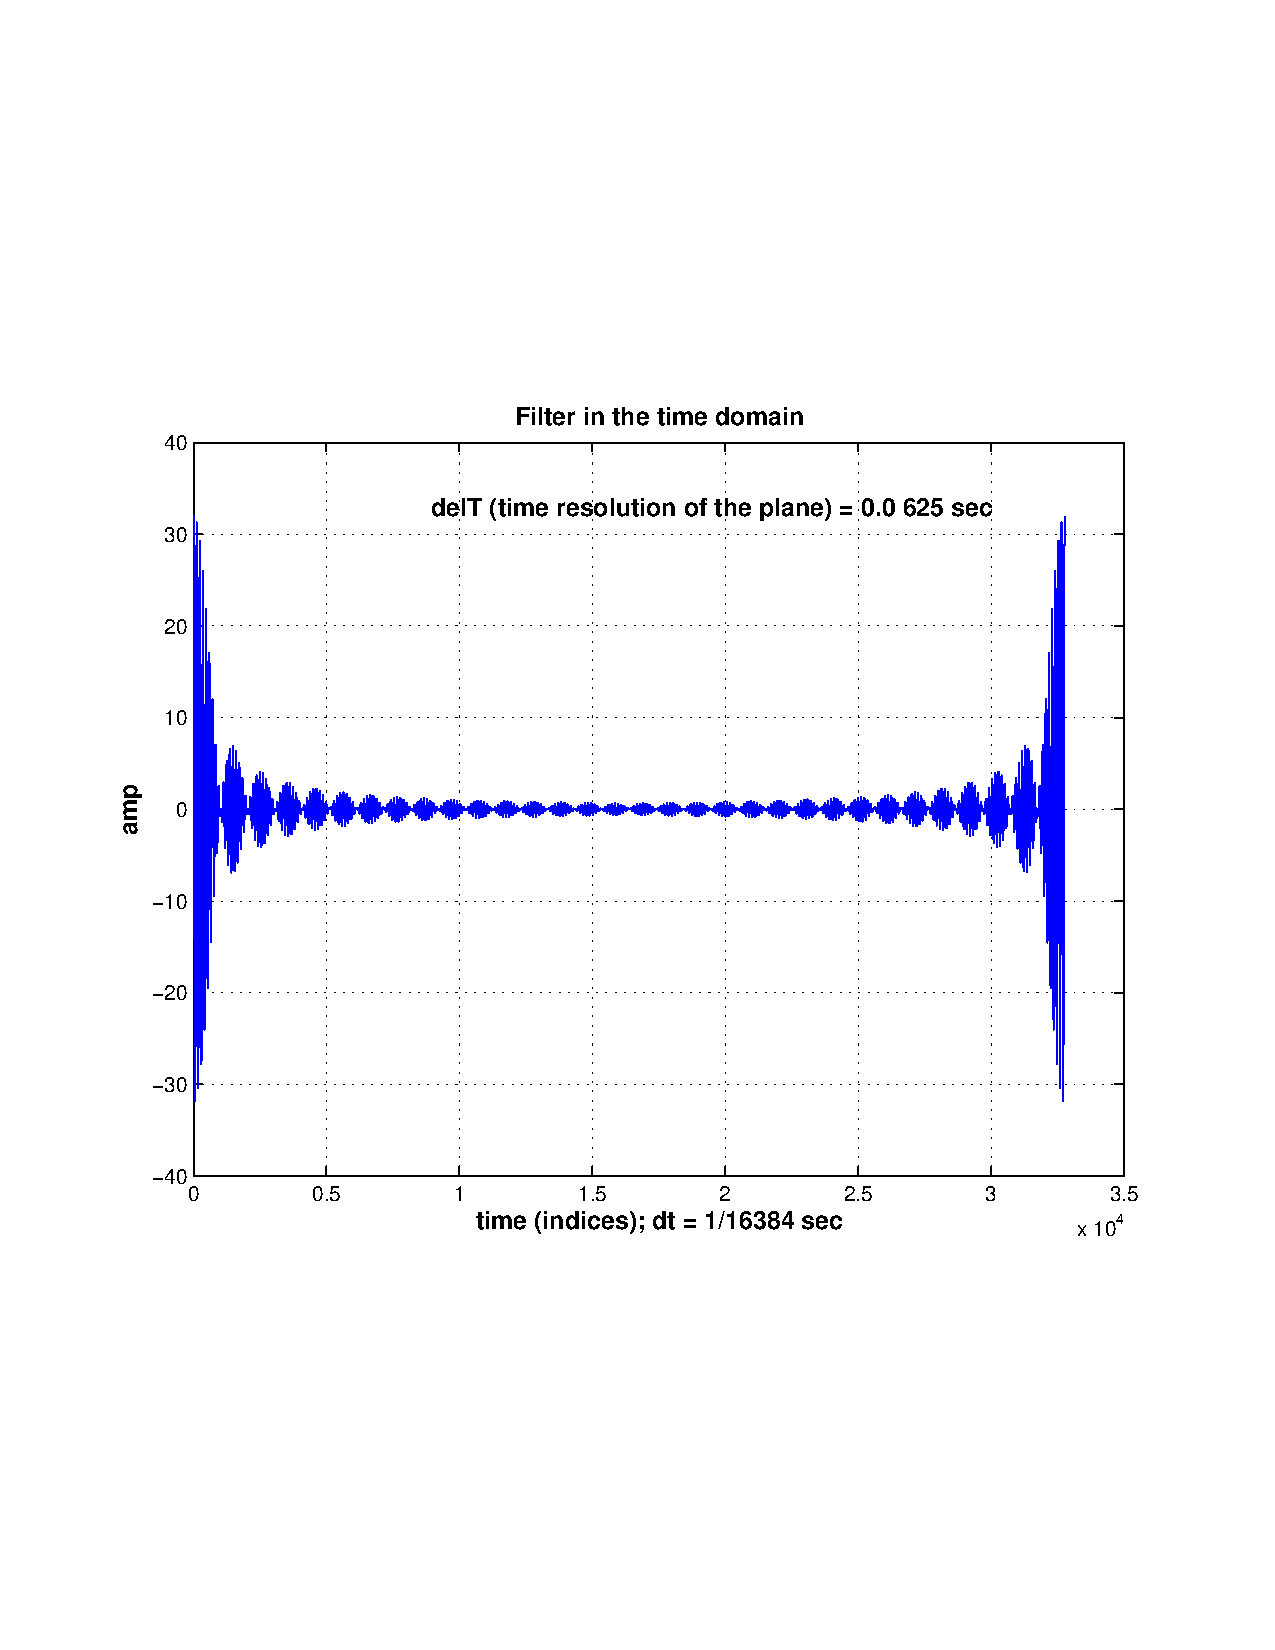
\includegraphics[width=0.9\textwidth]{figures/timedomainfilter}
\caption{Filter in the time domain in a wrapped around fashion}
\label{fig:timedomainfilter}
\end{center}
\end{figure}
 
We can, however, start from this and construct a filter which
preferentially passes the appropriate frequencies \emph{and} has finite
duration in the time domain (Figure~\ref{fig:timedomainfilter_1} \&
Figure~\ref{fig:freqdomainfilter_1}).

\begin{figure}
\begin{center}
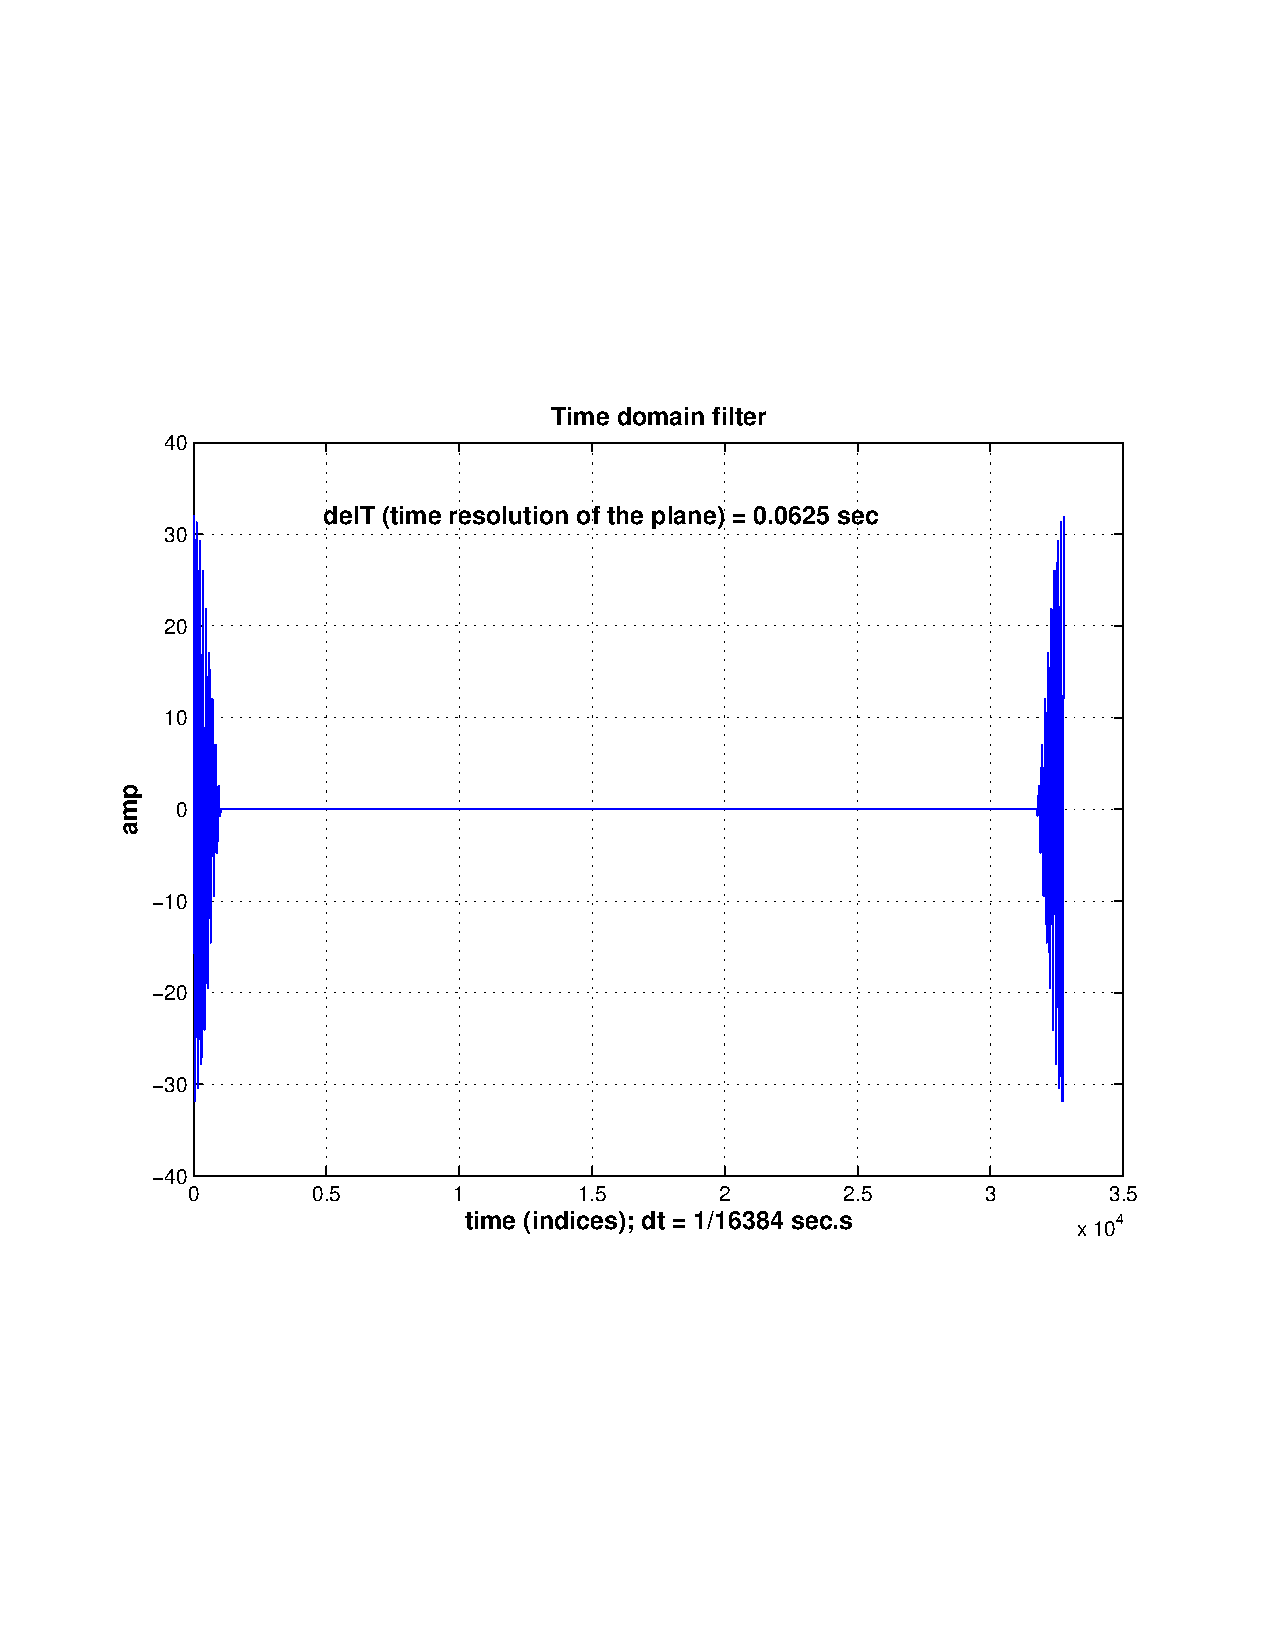
\includegraphics[width=0.8\textwidth]{figures/timedomainfilter_1}
\caption{Filter in the time domain}
\label{fig:timedomainfilter_1}
\end{center}
\end{figure}
\begin{figure}
\begin{center}
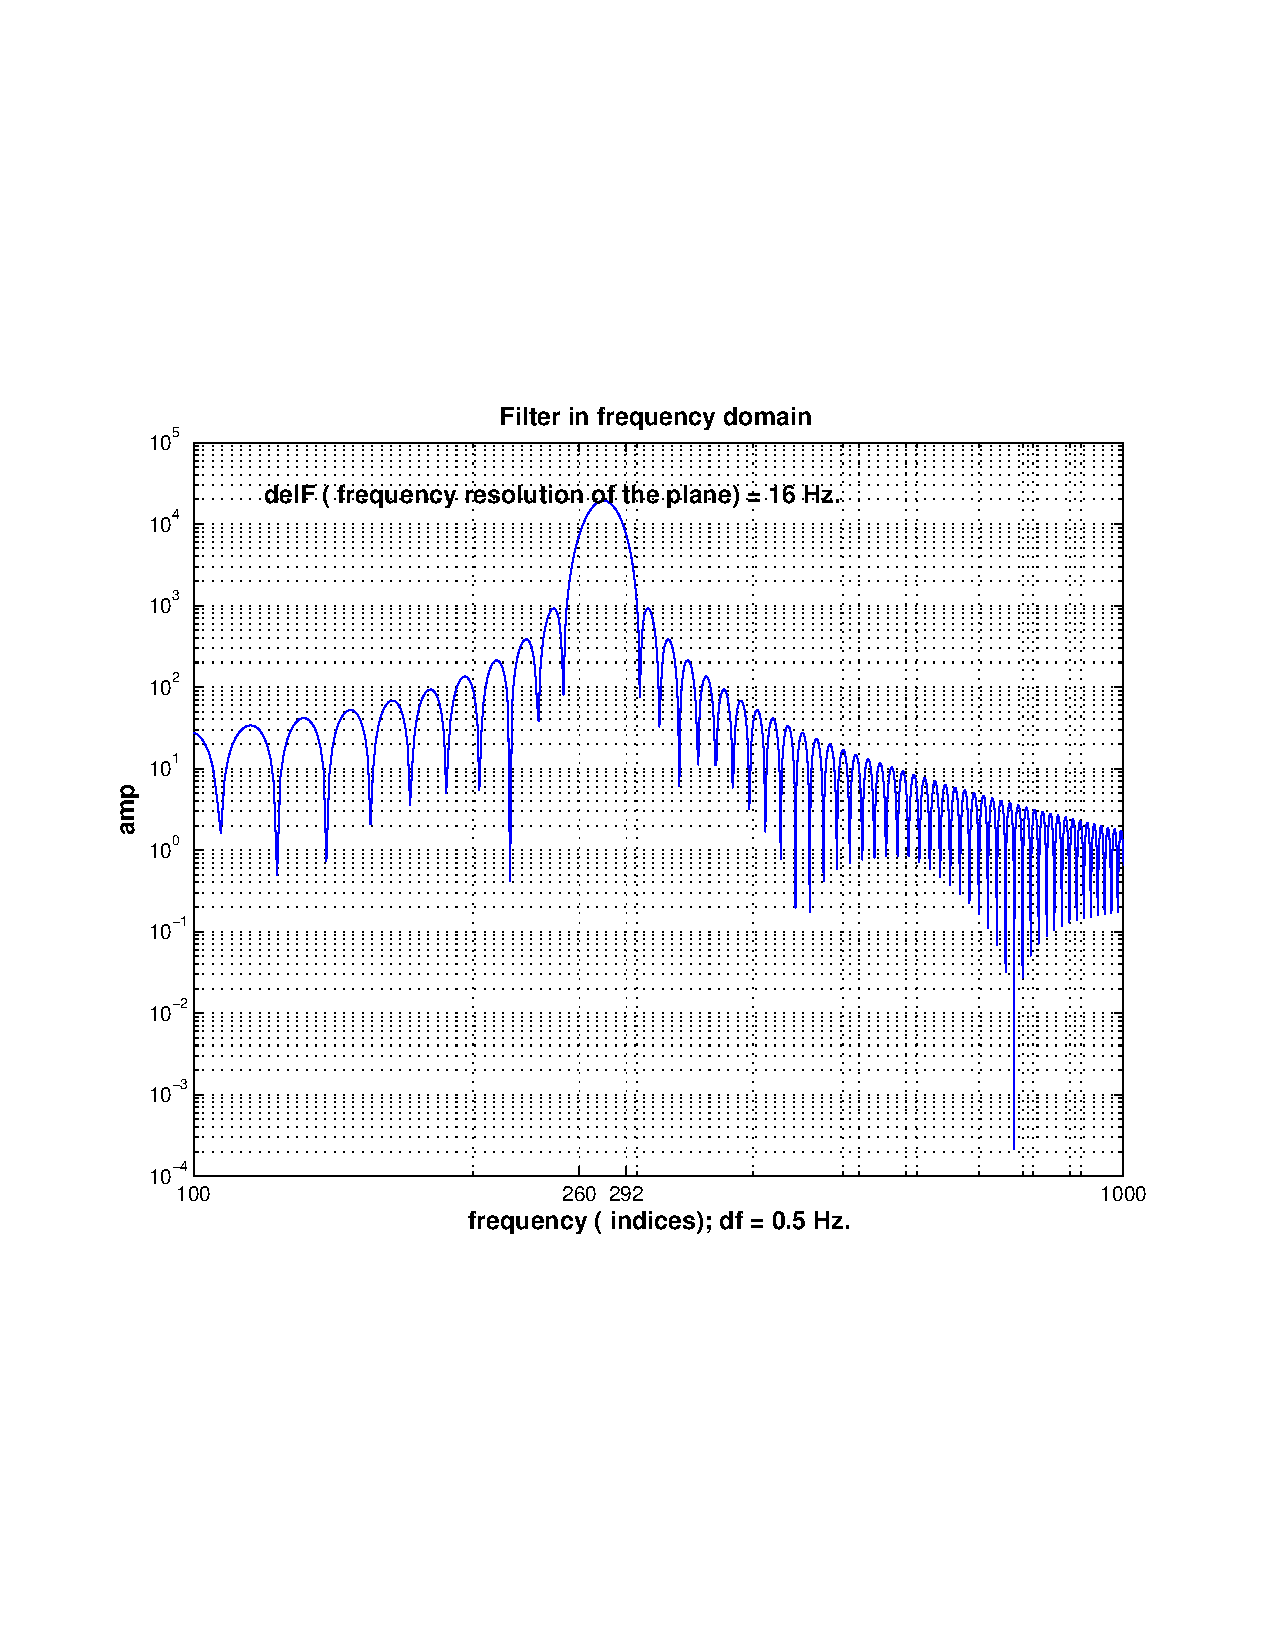
\includegraphics[width=0.8\textwidth]{figures/freqdomainfilter_1}
\caption{Filter in the frequency domain}
\label{fig:freqdomainfilter_1}
\end{center}
\end{figure}

Consider the rectangular band-pass in the frequency domain
\begin{eqnarray}
G(t) &=& \int_{-f_0 - b}^{-f_0} e^{2 \pi i f t} df  +
\int_{f_0}^{f_0+b}  e^{2 \pi i f t} df 
= 2 \int_{f_0}^{f_0+b} \cos ( 2 \pi f t ) df \\
&=& \frac{\sin[2\pi(f_0+b)t] - \sin[2 \pi f_0 t]}{\pi t} \; .
\end{eqnarray}
This is just the sum of a sine and cosine at
frequency $f_0$ modulated at frequency $b$.
Consequently,  the amplitude modulation has its first zero at
$t = 1/ (2 b)$ and we can use a truncated time-domain filter
\begin{equation}
\Theta(t - t_0; f_0 , b) = \left\{
\begin{array}{lrl}
\displaystyle{
\frac{\sin[2\pi(f_0+b)(t-t_0)] - \sin[2 \pi f_0 (t-t_0)]}{\pi (t-t_0)} 
} & \mbox{\ \ } & |t-t_0| < 1/(b)  \\
0 & & \textrm{Otherwise}
\end{array} \right. 
\label{eq:filter}
\end{equation}
which covers a time frequency volume $V = b (1/b) = 1$ and has its
peak at time $t_0$.   Notice that
\begin{equation}
\lim_{t\rightarrow t_0} \Theta(t - t_0; f_0 , b) = b\; .
\end{equation}

\subsubsection{The signal-to-noise}

The signal to noise for a filter determined by $f_0$ and $b$ can be
written as a function of the peak time $t_0$ as
\begin{equation}
\rho(t_0) = \frac{z(t_0)}{\sigma}
\end{equation}
where
\begin{equation}
z(t_0) = \int_{-\infty}^\infty \hat{s}(t) \Theta(t-t_0; f_0, b) 
dt
\end{equation} and $\sigma^2 = \langle |z(t_0)|^2 \rangle$.  The time
series $z(t_0)$ is most conveniently computed using Fourier
transforms,  therefore
\begin{equation}
z(t_0) = \int_{-\infty}^{\infty} \hat{s}(f) \tilde{\Theta}^\ast (f) 
e^{2 \pi i ft_0} df
\end{equation}

The Excess Power search then identifies triggers which may be
gravitational wave bursts using the following algorithm.  
We construct a single
time frequency plane and then search over all possible tiles of different
time durations and frequency bands.  One first decides the maximum 
frequency band and the maximum time duration that are to be tolerated in
the search.  The maximum frequency band determines the minimum duration
a tile requiring the time-frequency volume be $1$ and 
similarly the maximum time duration determines the minimum frequency band
of the tile.  The time frequency plane is then constructed with a 
time-frequency resolution finer by at least a factor of $2$ compared to
the minimum resolutions of the tiles.  As a concrete example,  
suppose the maximum allowed time duration of a tile is 
$\Delta T sec = 2^{-(a+1)} sec$  and the maximum frequency band is 
$\Delta F Hz = 2^{(b-1)} Hz$.  This implies the minimum duration of a tile 
in the search will be  $\Delta t^{tile} sec = 2^{-(b-1)} sec$  and the 
minimum frequency band will be  $\Delta f^{tile} Hz = 2^{(a+1)} Hz$.
 The time-frequency plane is then constructed with a timing resolution
of $\delta t sec = 2^{-b} sec.$ and a frequency resolution of 
$\delta f Hz = 2^a Hz$.

For each whitened segment $\hat{s}_k$, one constructs multiple channels,  
each of which is an inverse Fourier tranform of $\delta f Hz$ of data.  
Now suppose the bandwidth over which we want to search is $ F Hz$ and the 
time duration is $ T sec $. Therefore there will be
$n_{chan} = \frac{ F Hz}{\delta f Hz}$ channels and $n_{timebins} 
= \frac{T sec}{ \delta t sec}$ timebins in each channel. 
$n_{timebins} \times n_{chan}$ number of elements will then represent 
this time-frequency plane.

If we consider a channel whose low frequency index is $k_0$ 
(where $k_0 = \frac{flow Hz}{ \delta f Hz}$,  $flow Hz$ being the low 
frequency of the channel) and the channel width in number of sample 
points is $ b = \frac{\delta f Hz }{\Delta f Hz} $ ($\Delta f Hz $ is the
 frequency resolution of the fully sampled frequency series),  it's elements 
can be represented as:
\begin{equation}
z_{j}(k_0,  b) = \sum_{k=0}^{N-1}  \hat{s}_k \tilde{\Theta}_k^\ast(k_0,  b) 
e^{2 \pi ijk/N},
\label{eq:tfplanecountspoints}
\end{equation}  where $j = 0,\cdots, N-1$.  Note,  the timing
resolution of $z_j(k_0,  b)$ is equal to that of the sampled detector 
data $s_j$.  The elements of the time-frequency plane corresponding to this 
particular channel $z_j(k_0,  b)$ will then be 
\begin{equation}
Z_J(k_0,  b)   = z_{Jn_t}(k_0,  b),
\end{equation} where $n_t = \frac{\delta t sec}{\Delta sec}$ are the number 
of sample points in one time-frequency plane time bin ($\Delta sec$ being 
the full sampling rate of the timing series)  and $J = 0, \cdots, 
n_{timebins} - 1$.

Each channel is normalised so that a sample point in the channel represents
a Gaussian random variable with zero mean and unit variance. The normalisation 
constant is given by 
\begin{equation}
\sigma^2(k_0,  b) = \langle z_j^2(k_0, b) \rangle = \sum_{k=0}^{N-1}
\sum_{l=0}^{N-1}\langle \hat{s}_k \hat{s}_l^\ast \rangle 
\tilde{\Theta}_k^\ast(k_0,  b) \tilde{\Theta}_l(k_0,  b) e^{2 \pi ij(k-l)/N},
\end{equation}
where $\langle \hat{s}_k \hat{s}_l^\ast \rangle = 2\delta(k-l)$.  Hence,  the 
normalisation simplifies to 
\begin{equation}
\sigma^2(k_0,  b) = 2\sum_{k=0}^{N-1}\mid \tilde{\Theta}_k^2(k_0,  b) \mid .
\end{equation}

Now suppose we have a channel with the same low frequency $k_0$ but
twice the frequency band,  i.e. $2b$ compared to the previous channel.
We therefore have 
\begin{equation}
z_j(k_0,  2b) = \sum_{k=0}^{N-1}  \hat{s}_k \tilde{\Theta}_k^\ast(k_0,  2b) 
e^{2 \pi ijk/N},
\end{equation}
where $\tilde{\Theta}_k^\ast(k_0,  2b)$ from Eq~\ref{eq:filter} is given by
\begin{equation}
\tilde{\Theta}(k_0,  2b) = \sum_{j=0}^{N-1}\frac{sin[2\pi/N(k_0 + 2b)j] 
- sin[2\pi/Nk_0j]}{\pi j \Delta}e^{-12\pi jk/N}
\end{equation}
However we can write
\begin{equation}
sin[2\pi/N(k_0 + 2b)j] - sin[2\pi/Nk_0j] = sin[2\pi/N(k_0 + b)j] - 
sin[2\pi/Nk_0j] + sin[2\pi/N(k_0 + 2b)j] - sin[2\pi/N(k_0 + b)j]
\label{eq:sines}
\end{equation}
and hence we get
\begin{equation}
\tilde{\Theta}(k_0,  2b) = \tilde{\Theta}(k_0,  b) + 
\tilde{\Theta}(k_0 + b,  b)
\end{equation}
which implies
\begin{equation}
z_j(k_0,  2b) = z_j(k_0,  b) + z_j(k_0 +b,  b).
\end{equation}
This is shown in Fig~\ref{fig:sumfilters}.  
\begin{figure}
\begin{center}
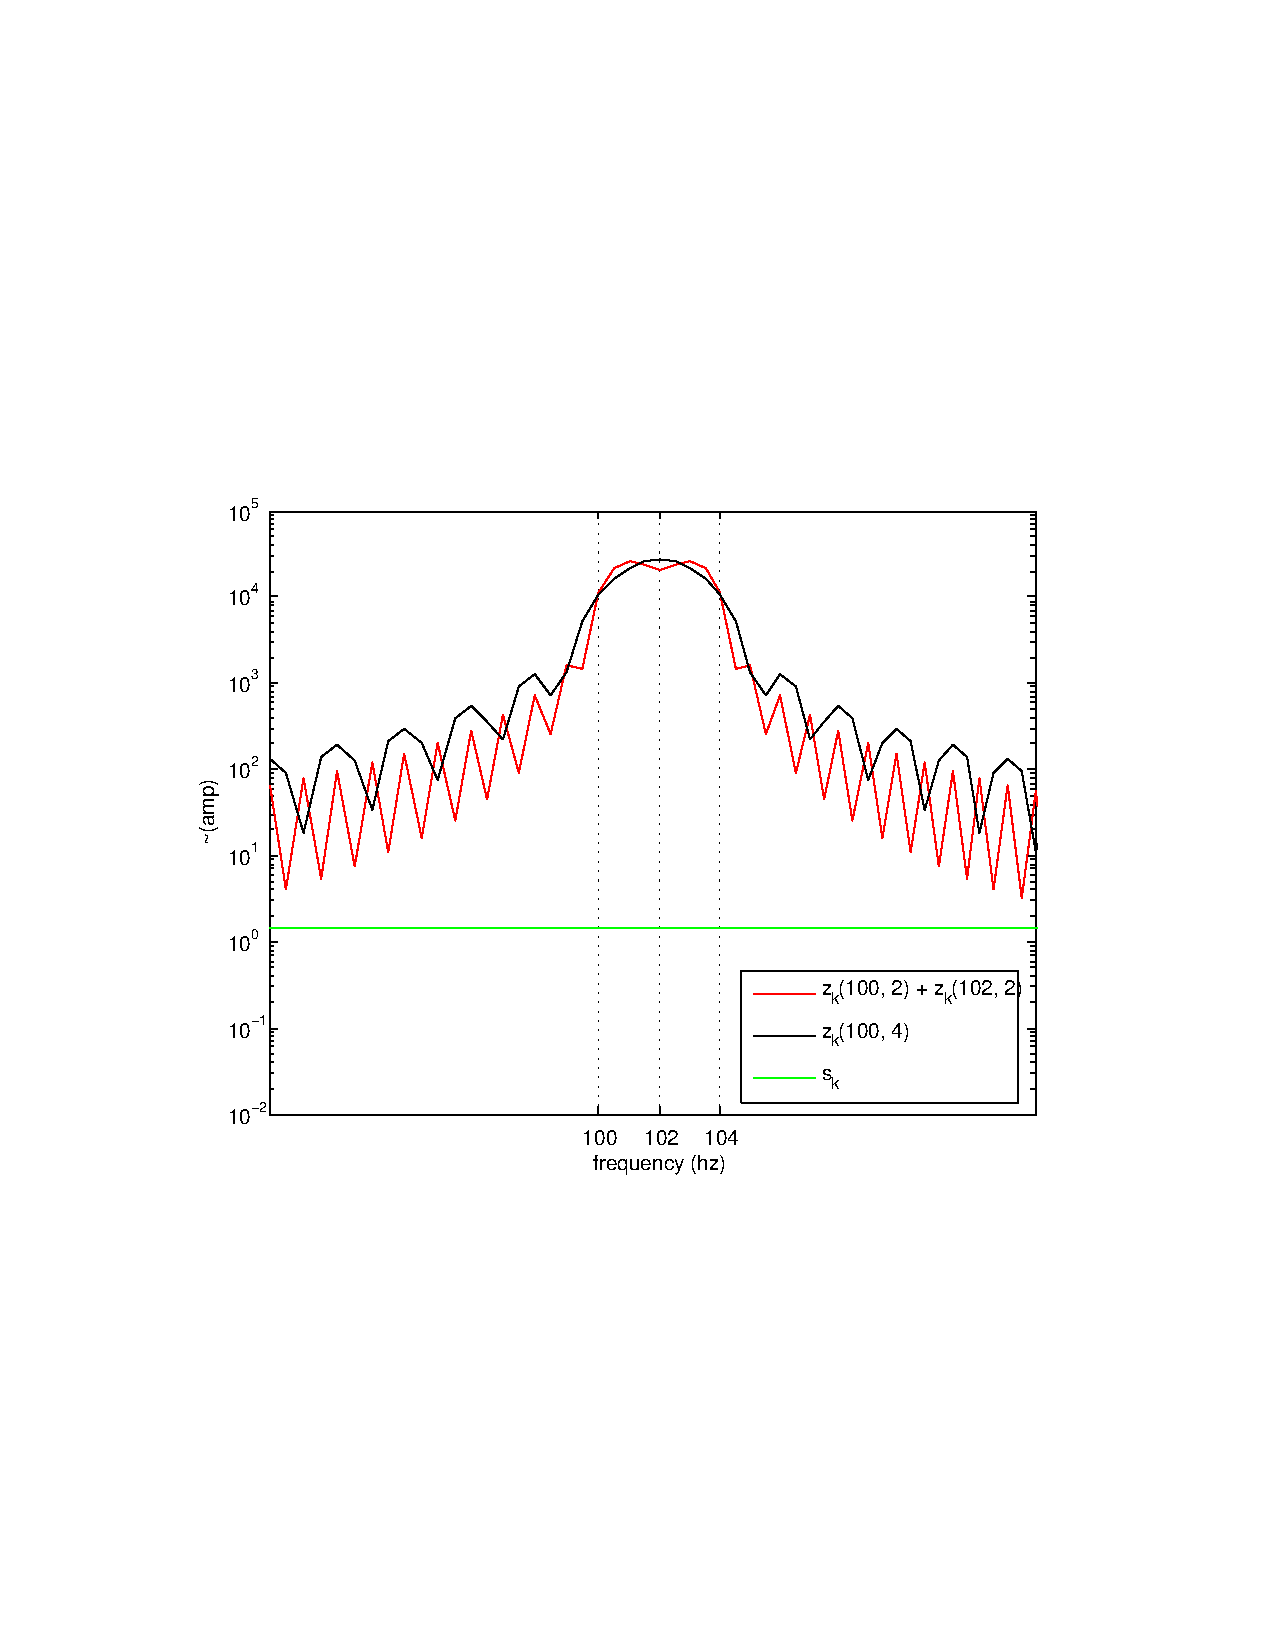
\includegraphics[width=0.9\textwidth]{figures/sumoffilters}
\caption{Response to a 4 hz wide filter compared to the sum of two 2 Hz wide 
filters}
\label{fig:sumfilters}
\end{center}
\end{figure}
The data used to generate this plot is a delta function in the time domain
(so that it is a flat line in the frequency domain, as shown by the green 
curve in the Fig~\ref{fig:sumfilters}). The black curve shows the output when 
the channel width is $4 Hz$, while the red curve shows the sum of the output 
of two $2 Hz$ wide channels. 


The corresponding normalisation,  
\begin{equation}
\sigma^2(k_0,  2b) = \sigma^2(k_0,  b) + \sigma^2(k_0+b,  b) + 
2\sum_{k=0}^{N-1}\tilde{\Theta}_k^\ast(k_0,  b)\tilde{\Theta}_k(k_0 + b,  b)
\label{eq:norm}
\end{equation}
The filter being orthogonal(almost),  the cross term in Eq~\ref{eq:norm} 
will be negligible.  

A tile in this plane can be denoted as $\tau =\{J_1, \Delta n_t, K_1, \Delta 
n_f\}$,  where $J_1$ and $K_1$ represent the indices corresponding to the 
start time and start frequency of the tile respectively while $\Delta n_t$ 
and $\Delta n_f$ are respectively the time and frequency bins.  The degrees 
of freedom assosciated with $\tau$ will then be $dof_{\tau} = 2 \times n_t 
\times \Delta t \times n_f \times \Delta f $.  Requiring that there are at 
least two sample points in the unit time-frequency volume tile we see that 
the time-frequency sample points have to be picked at every  $\Delta t^{tile} 
sec = 1 / (2 \times n_f \times \delta f)$,  where $\delta f$ is the 
time-frequency plane frequency resolution.  In terms of sample points then 
every $\Delta t^{tile} / \delta t $ sample point has to be considered while 
calculating the power of the tile.  Now,  $\Delta t^{tile} / \delta t = 
\frac{1}{(2 \times n_f \times \delta f) \times \delta t} = n_t / dof_{\tau}$  
and the power in the tile will then be 
\begin{equation}
\varepsilon_{\tau} = \sum_{n=0}^{dof_{\tau}-1}\frac{(\sum_{k=K1}^{\Delta 
n_f -1}Z_{[J_1 + n\frac{n_t}{dof_{\tau}}]}(k,b))^2}{\sum_{k=K1}^{\Delta 
n_f -1}\sigma^2(k,b)}.
\end{equation}

In Gaussian noise,  the power in a given tile is $\chi^2$-distributed
with $2 V$ degrees of freedom where $V$ is the time-frequency volume
of the tile.    A burst trigger is identified if the probability of
obtaining the excess power in a tile from Gaussian noise is smaller
than some threshold $\alpha$.   For large bursts in the data stream,
many tiles can be identified as triggers with different sizes and
aspect ratios.   When the search over a particular segment is
complete,   triggers are clustered and the clustering is described in 
Section~\ref{section:clustering} .
\clearpage

\subsubsection{$h_{rss}$ Estimation}
The way we estimate $h_{rss}$ corresponding to a tile $\tau$ is described 
here.  By definition,
\begin{equation}
h_{rss}^2 =  \int h^2(t)dt = \sum h^2_j \delta t,
\end{equation}
where $h_j$ is the gravitational wave strain data. This in the frequency 
domain is related to the data in counts units(which has been used for all 
the documentation till now) by: 
\begin{equation}
\tilde h_k = R_k \tilde s_k,
\end{equation}  
where $R_k$ is the detector response function with units $strain / counts$ 
while the unit of $h_k$ is strain and of $s_k$ is counts.  In terms of the 
normalised data:
\begin{equation}
\tilde h_k = \frac{R_k \sqrt P_k}{2\sqrt {\Delta f }}\hat s_k
\end{equation}
The corresponding time-frequency plane points are 
\begin{eqnarray}
H_j(k_0, b) &=& \frac{1}{N}\sum_{k=0}^{N-1}\tilde h_k \tilde 
\Theta^\ast_k(k_0, b)e^{i 2 \pi jk/N} \\
&=& \frac{1}{N}\sum_{k=0}^{N-1} \frac{R_k(k_0, b)\sqrt P_k(k_0, b)}
{2\sqrt {\Delta f }}\hat s_k \tilde \Theta^\ast_k(k_0, b)e^{i 2 \pi jk/N}
\end{eqnarray}
For the present implementation we have assumed 
\begin{itemize}
\item the response and the average spectrum can be replaced by their average 
values over the channel width and 
\item effect of the response phase is negligible.  
\end{itemize}
So we can pull their contributions out of the sum and let us denote that by 
$F(k_0, b) = \frac{R_k(k_0, b)\sqrt {P_k(k_0, b)}}{2N\sqrt {\Delta f }}$.
Therefore we get 
\begin{equation}
H_j(k_0, b) = F(k_0, b) z_j(k_0, b) , 
\end{equation} 
where $z_j$ are the time-frequency sample points obtained by using the data 
in counts as given in Eq~\ref{eq:tfplanecountspoints}.  The $h_{rss}$ 
corresponding to the tile $\tau$ will then be 
\begin{equation}
h_{rss}^2 = \sum_{n=0}^{dof_{\tau}-1}(\sum_{k=K1}^{\Delta n_f - 1}
F(k,b)Z_{[J_1 + n\frac{n_t}{dof_{\tau}}]}(k,b))^2\Delta t^{tile}.
\end{equation}
How well can we estimate the $h_{rss}$ under the above assumptions
are shown by Fig~\ref{fig:hrss}.  We have plotted the injected
$h_{rss}$ on the x-axis and the estimated $h_{rss}$ on the y-axis. Ideally
we would expect them to lie on a straight line at 45 degrees with the
x-axis(as marked by the red line in the plot). 
\begin{figure}
\begin{center}
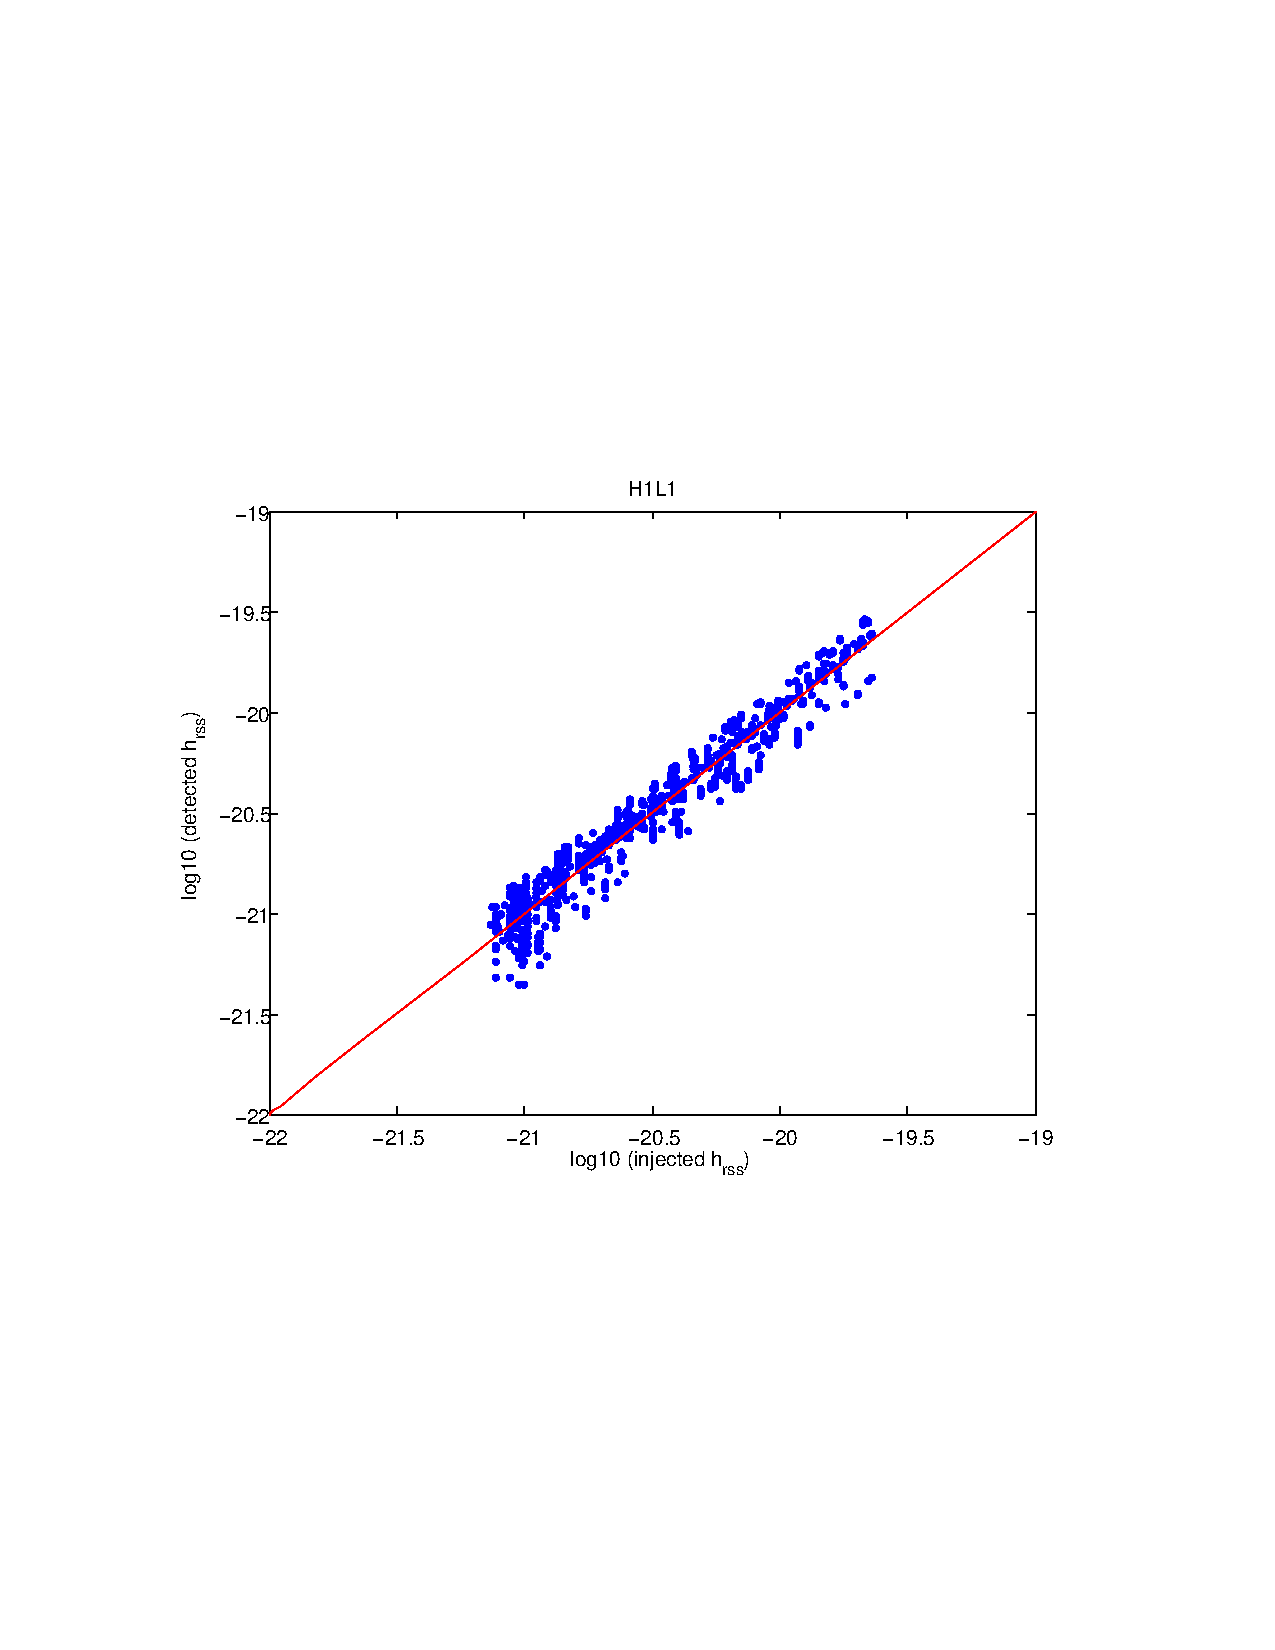
\includegraphics[width=0.9\textwidth]{figures/inj_det_hrss}
\caption{Injected vs Detected $h_{rss}$}
\label{fig:hrss}
\end{center}
\end{figure}
\clearpage
 
\subsection{Time Domain Segmentation}
The excess power analysis code does not process the input data as a
continuous time series;  rather the time series is split into a sequence of
discrete ``analysis windows'', which are each analyzed individually.  To
account for the possibility of a burst event stradling the boundary between
two analysis windows, successive windows are staggered in such a way that
they overlap one another in time.  In this way, a burst event occuring on
the boundary of one window will (typically) be centred in the next.

Because edge effects at various stages of the analysis can corrupt the
beginning and end of the analysis window, the actual quantity of data
extracted from the input time series to form a window is twice the amount
that is analyzed.  Only results from the central half of the window are
retained, with the first and last quarters of each window being discarded.
The arrangement is shown in the following diagram.
\begin{center}
\begin{picture}(0,0)%
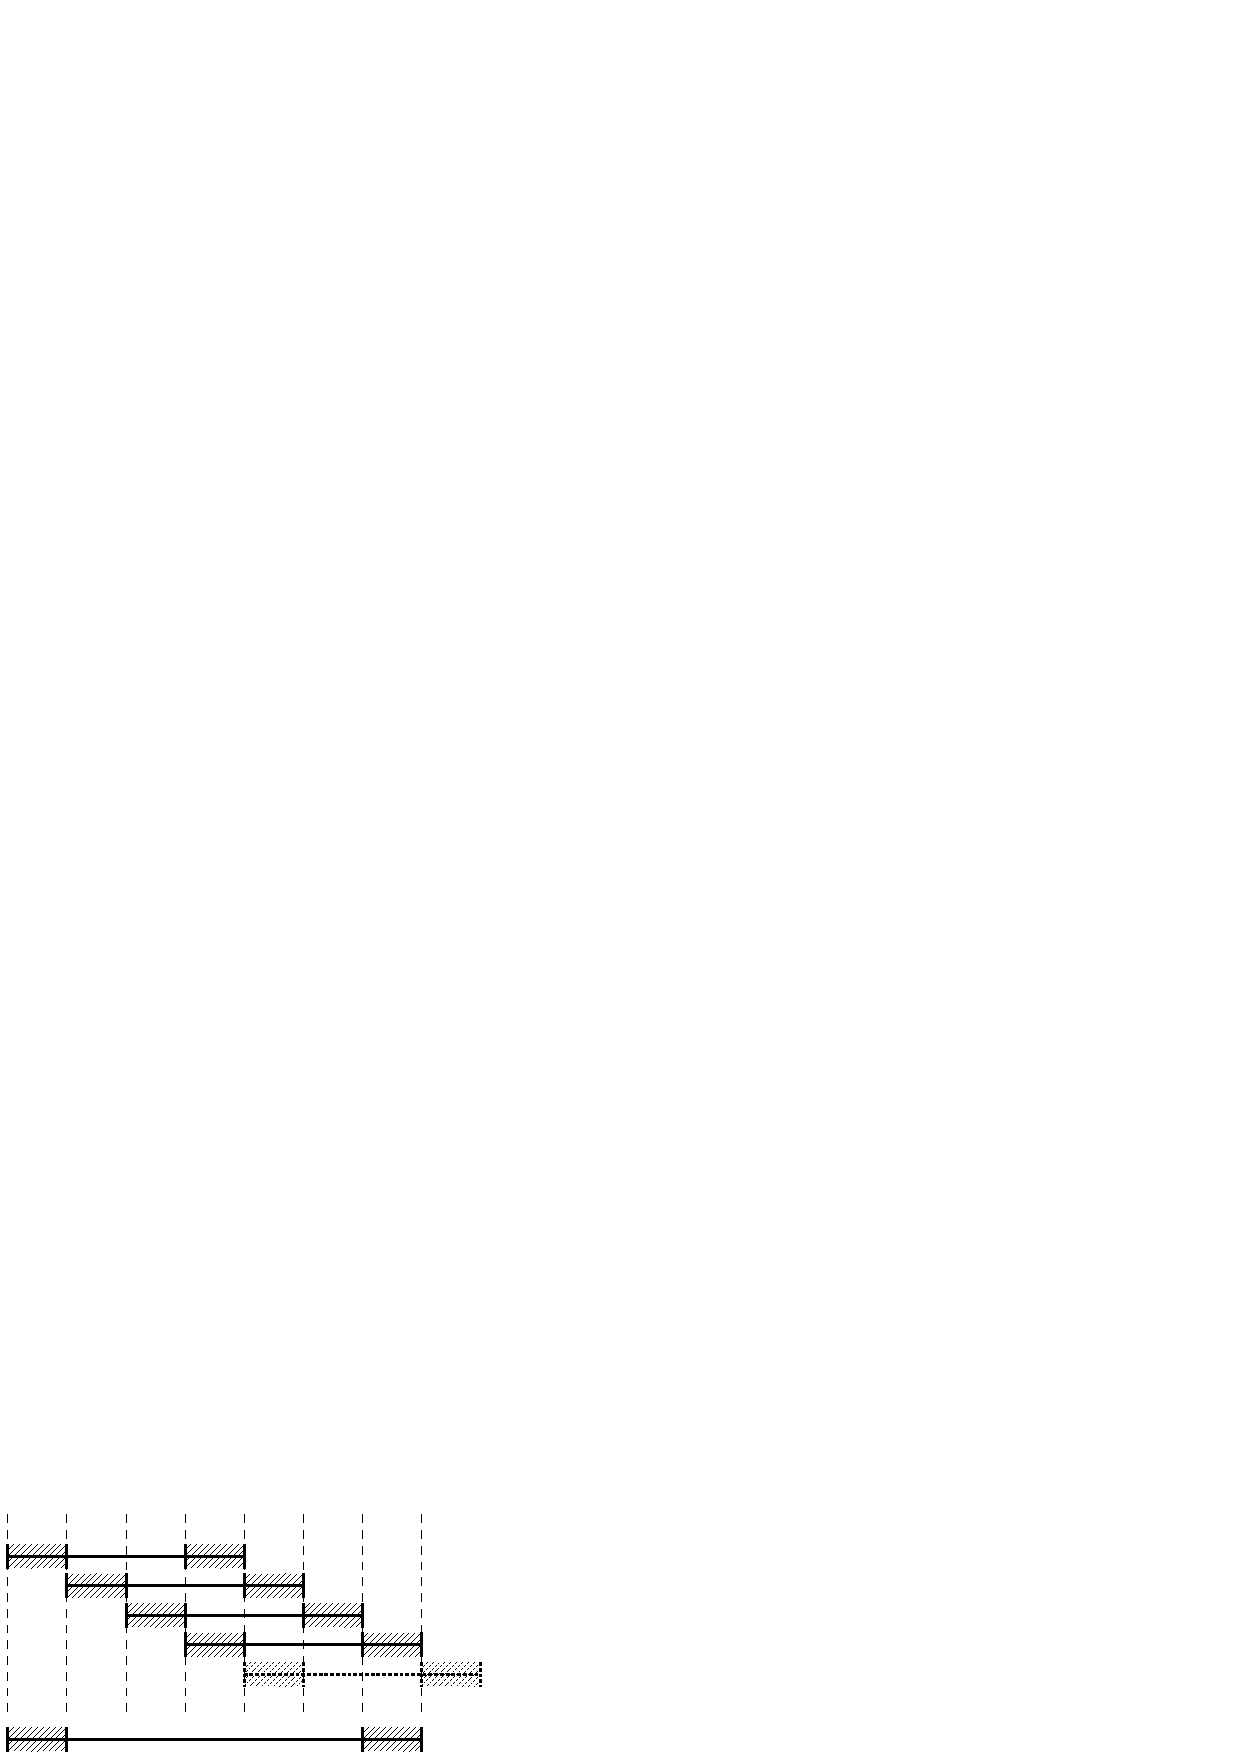
\includegraphics{figures/power/windows.fig.pdf}%
\end{picture}%
\setlength{\unitlength}{4144sp}%
%
\begingroup\makeatletter\ifx\SetFigFont\undefined%
\gdef\SetFigFont#1#2#3#4#5{%
  \reset@font\fontsize{#1}{#2pt}%
  \fontfamily{#3}\fontseries{#4}\fontshape{#5}%
  \selectfont}%
\fi\endgroup%
\begin{picture}(3194,1329)(-21,-253)
\put( 46,929){\makebox(0,0)[lb]{\smash{{\SetFigFont{10}{12.0}{\familydefault}{\mddefault}{\updefault}0}}}}
\put(1846,929){\makebox(0,0)[lb]{\smash{{\SetFigFont{10}{12.0}{\familydefault}{\mddefault}{\updefault}32768}}}}
\put(3151,434){\makebox(0,0)[lb]{\smash{{\SetFigFont{10}{12.0}{\familydefault}{\mddefault}{\updefault}\(\cdots\)}}}}
\end{picture}%

\end{center}
Here we see a discrete time series (represented by the bottom-most
horizontal line) that contains 57344 samples.  It has been divided into a
sequence of four analysis windows, each containing 32768 samples.  A fifth,
greyed-out, analysis window is shown to indicate where the next window in
the sequence would start.  In the analysis of each window, the first and
last 8192 samples (first and last quarter) are discarded as indicated by
the crossed-out sections in each window.  In this particular example, each
window is shifted 8192 samples (also equal to one quarter of the window
length) from the start of the previous window.  This choice of window
length and window shift causes the sections of each window that are
actually searched for events (the sections that are not crossed out) to
overlap their neighbours by half of their own width.  This is the typical
mode of operation for the search code.  Notice that the first and last
quarter window length of the complete time series (the cross-out sections
in the bottom line) are \emph{not} analyzed, as they are discarded from the
only analysis windows in which they appear.

The excess power code whitens the input time series using an estimate of
the instrument's noise power spectral density (PSD).  The estimated noise
PSD is computed by averaging the PSDs from a number of successive analysis
windows.  The noise PSD is not estimated by averaging over the entire time
series in order to allow the code to track the (possibly) changing
character of the instrument's noise.  For convenience, the user is
permitted to enter the number of samples that should be used to estimate
the PSD.  The number of samples entered should correspond to the time for
which the instrument's noise can be approximated as stationary for the
purpose of the excess power analysis.  Since, however, the actual
estimation procedure involves averaging over an integer number of analysis
windows, it is necessary for the number of samples selected to correspond
to the boundary of an analysis window.  For convenience,
\prog{lalapps\_power} will automatically round the value entered down to
the nearest analysis window boundary.

The LAL function \function{EPSearch()} performs the parts of the analysis
described above.  It is given a time series that it divides into analysis
windows, which it uses to estimate the noise PSD.  Using the estimated
noise PSD, it whitens each analysis window and then searches them for burst
events.  Only the analysis windows within the data used to estimate the
noise PSD are whitened using that estimate.  Once those windows have been
searched for burst events, \function{EPSearch()} returns to the calling
procedure which then extracts a new time series from the input data and the
process repeats.  The parameter provided via the command line option
\option{--psd-average-points} sets the length of the time series that is
passed to \function{EPSearch()}.

As successive time series are passed to \function{EPSearch()}, in order for
the first analysis window to correctly overlap the last window from the
previous time series --- i.e.\ to ensure the same overlap between analysis
windows in neighbouring time series as exists between neighbouring windows
within a series --- it is necessary for the latter time series to begin
$(\mbox{\parm{window length}} - \mbox{\parm{window shift}})$ samples before
the end of the former series.  The arrangement is shown in the following
figure.
\begin{center}
\begin{picture}(0,0)%
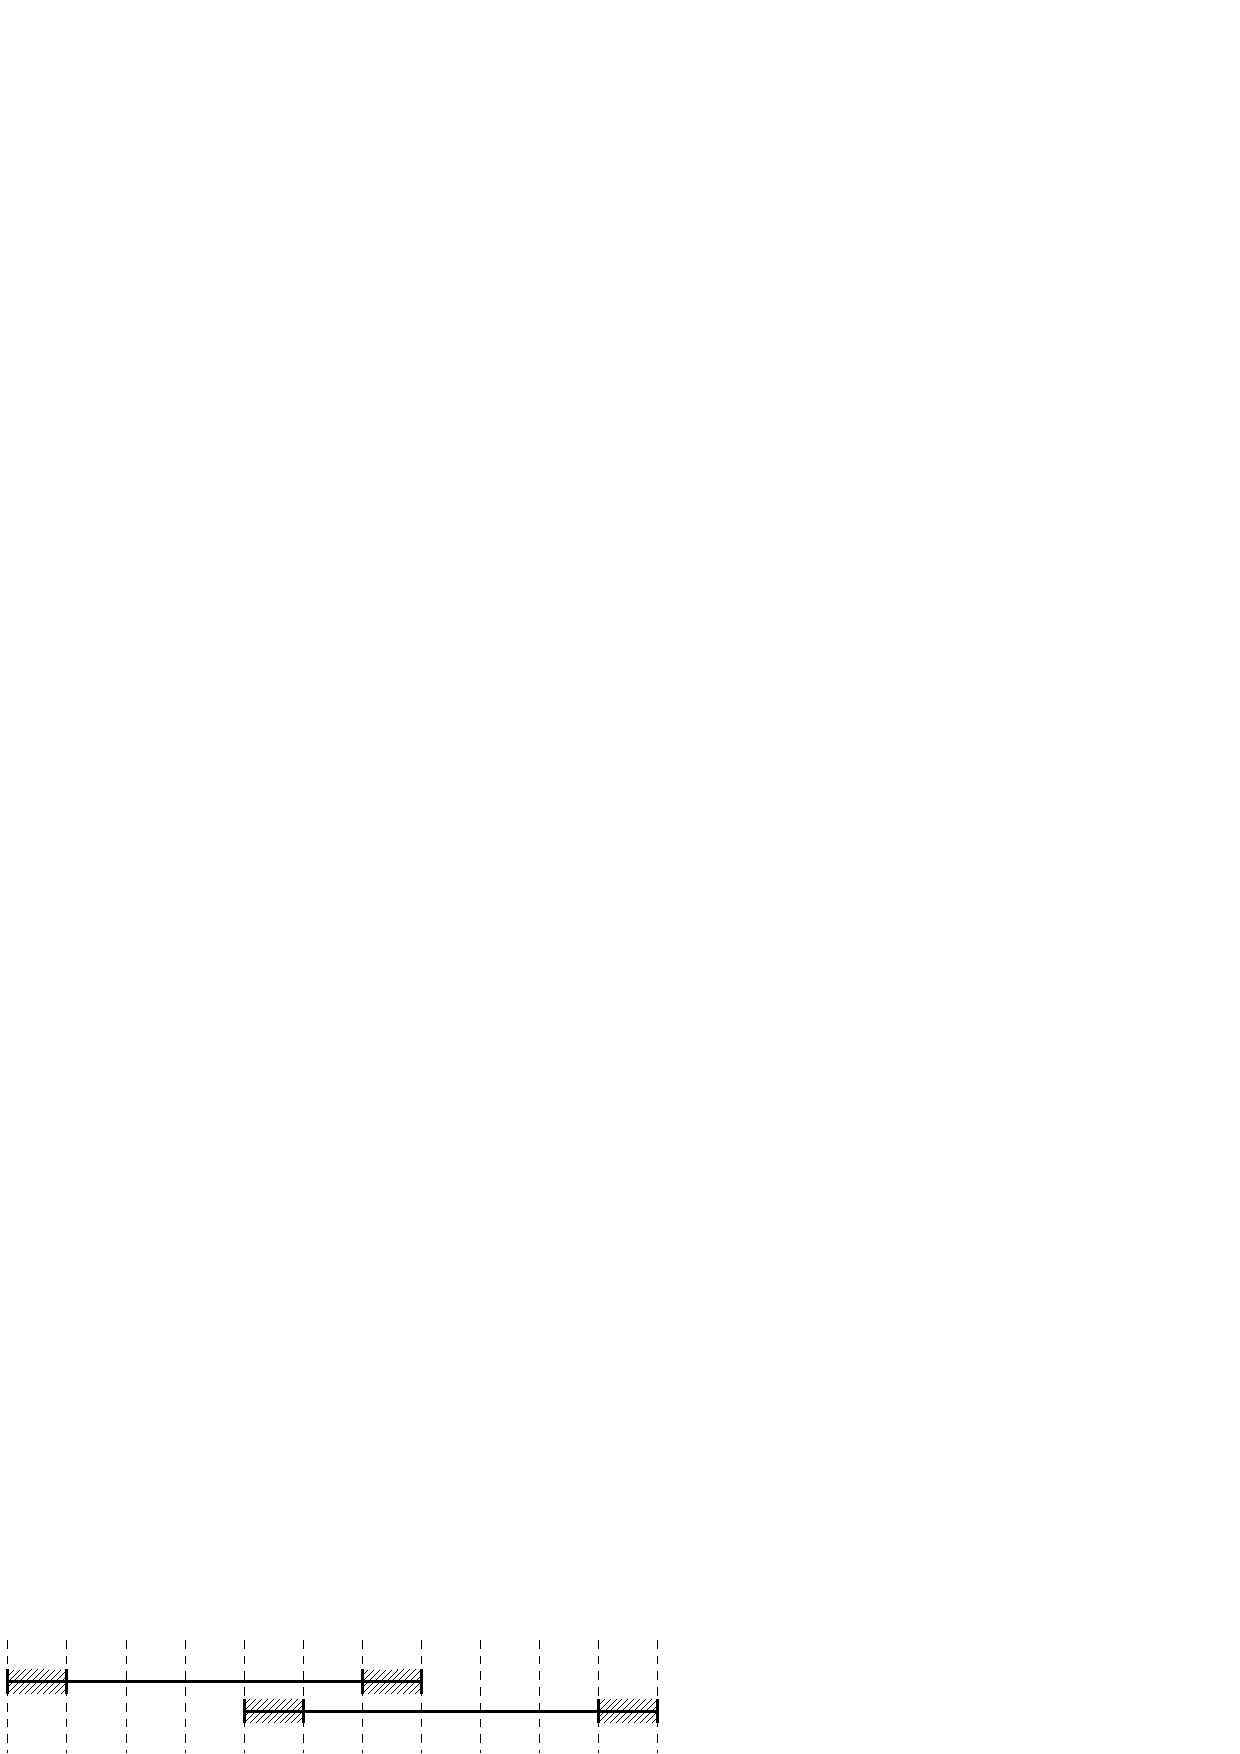
\includegraphics{figures/power/psds.fig.pdf}%
\end{picture}%
\setlength{\unitlength}{4144sp}%
%
\begingroup\makeatletter\ifx\SetFigFont\undefined%
\gdef\SetFigFont#1#2#3#4#5{%
  \reset@font\fontsize{#1}{#2pt}%
  \fontfamily{#3}\fontseries{#4}\fontshape{#5}%
  \selectfont}%
\fi\endgroup%
\begin{picture}(5364,1032)(-59,197)
\put(-44,1109){\makebox(0,0)[lb]{\smash{{\SetFigFont{10}{12.0}{\familydefault}{\mddefault}{\updefault}0}}}}
\put(1756,1109){\makebox(0,0)[lb]{\smash{{\SetFigFont{10}{12.0}{\familydefault}{\mddefault}{\updefault}32768}}}}
\put(3106,1109){\makebox(0,0)[lb]{\smash{{\SetFigFont{10}{12.0}{\familydefault}{\mddefault}{\updefault}57344}}}}
\put(4906,1109){\makebox(0,0)[lb]{\smash{{\SetFigFont{10}{12.0}{\familydefault}{\mddefault}{\updefault}90112}}}}
\end{picture}%

\end{center}
Here we see two of the time series from the first diagram above, each of
which is to be passed to \function{EPSearch()} for analysis.  To see why
the overlap between these two time series must be chosen as it is, refer to
the first diagram above to see where the greyed-out fifth analysis window
was to be placed.  That is where the first analysis window in the second
time series here will be placed.

Prior to looping over the data one noise PSD estimation length at a time,
the data is passed through a conditioning filter.  To account for edge
effects in the filter, an amount of data set by the command line option
\option{--filter-corruption} is dropped from the analysis at both the
begining and end of the time series.  The arrangement is shown in the
following diagram.
\begin{center}
\begin{picture}(0,0)%
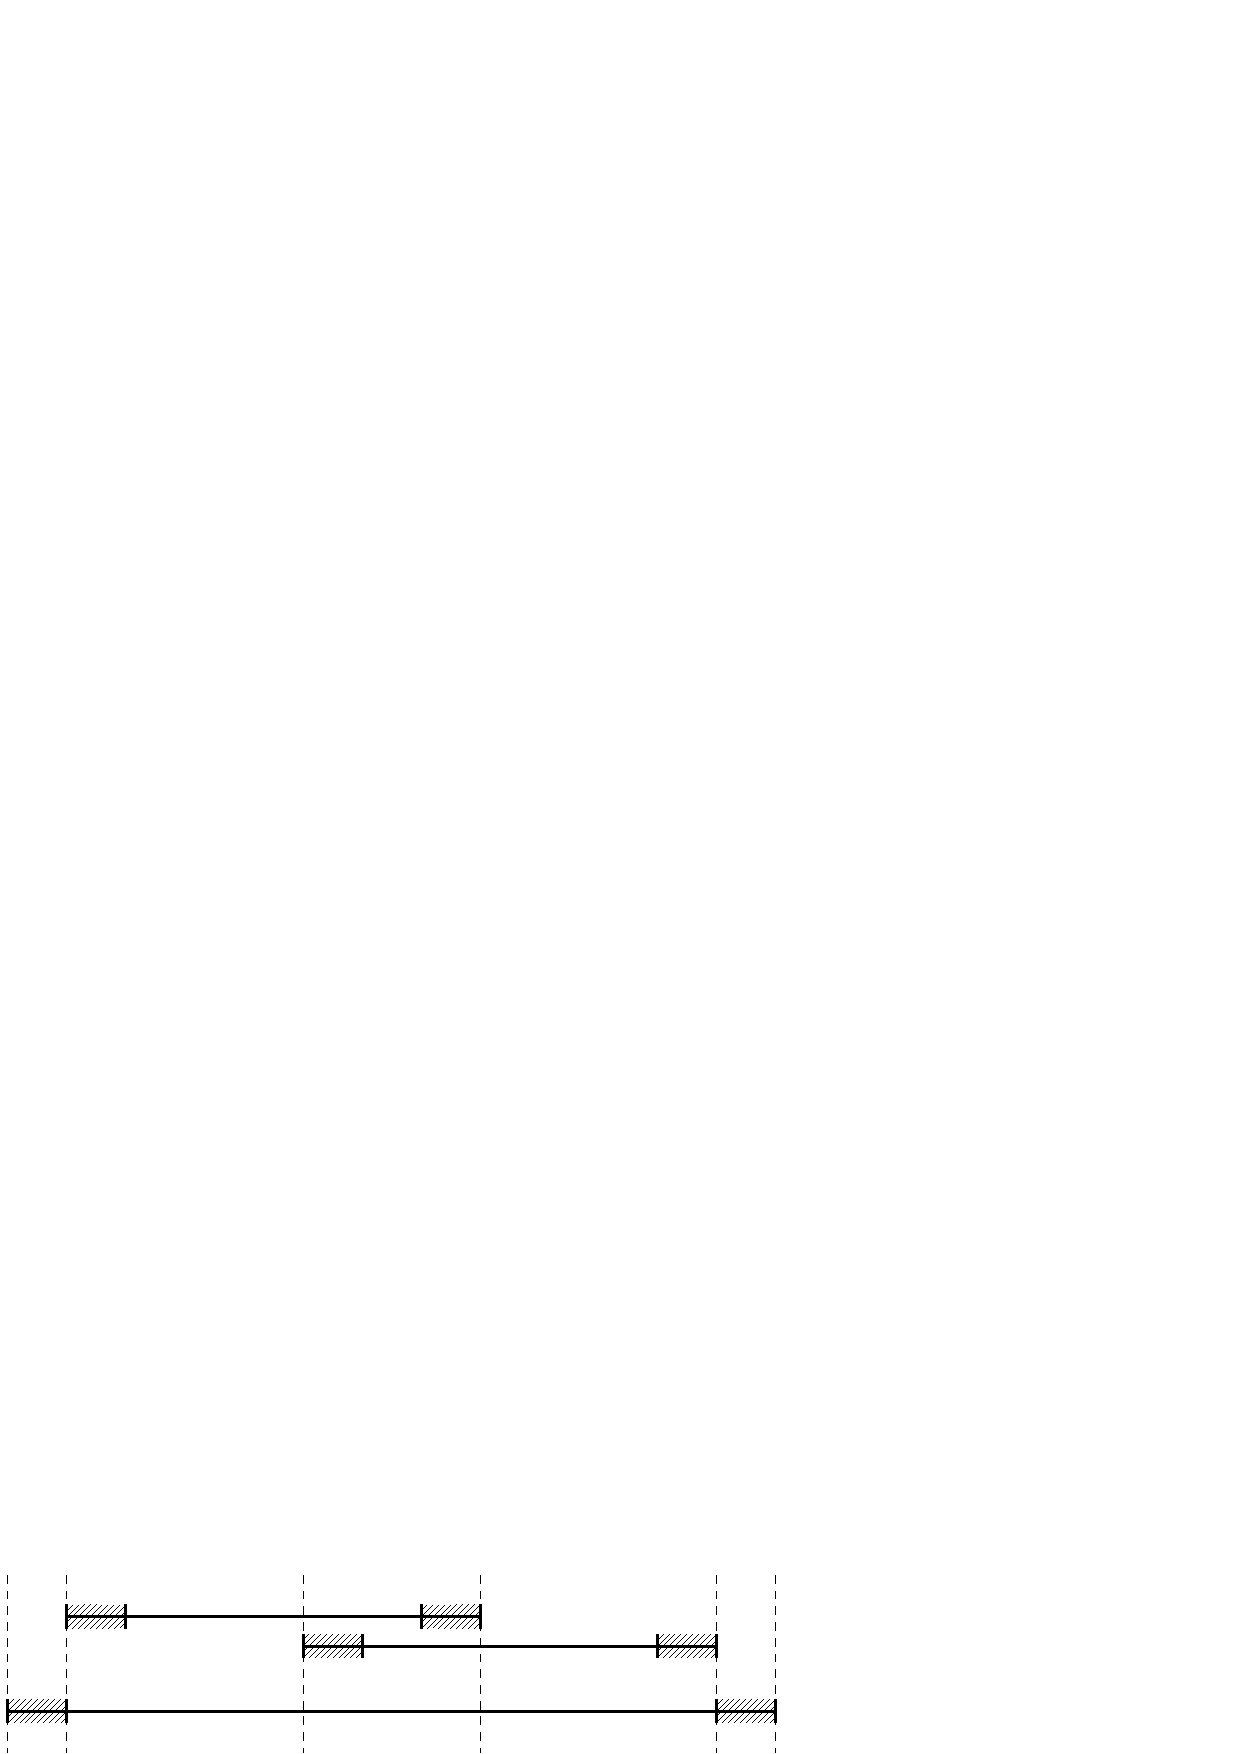
\includegraphics{figures/conditioning.fig.pdf}%
\end{picture}%
\setlength{\unitlength}{4144sp}%
%
\begingroup\makeatletter\ifx\SetFigFont\undefined%
\gdef\SetFigFont#1#2#3#4#5{%
  \reset@font\fontsize{#1}{#2pt}%
  \fontfamily{#3}\fontseries{#4}\fontshape{#5}%
  \selectfont}%
\fi\endgroup%
\begin{picture}(6341,1527)(-509,-298)
\put(-494,1109){\makebox(0,0)[lb]{\smash{{\SetFigFont{10}{12.0}{\familydefault}{\mddefault}{\updefault}0}}}}
\put(-44,1109){\makebox(0,0)[lb]{\smash{{\SetFigFont{10}{12.0}{\familydefault}{\mddefault}{\updefault}8192}}}}
\put(1756,1109){\makebox(0,0)[lb]{\smash{{\SetFigFont{10}{12.0}{\familydefault}{\mddefault}{\updefault}40960}}}}
\put(3106,1109){\makebox(0,0)[lb]{\smash{{\SetFigFont{10}{12.0}{\familydefault}{\mddefault}{\updefault}65536}}}}
\put(4906,1109){\makebox(0,0)[lb]{\smash{{\SetFigFont{10}{12.0}{\familydefault}{\mddefault}{\updefault}98304}}}}
\put(5356,1109){\makebox(0,0)[lb]{\smash{{\SetFigFont{10}{12.0}{\familydefault}{\mddefault}{\updefault}106496}}}}
\end{picture}%

\end{center}
The bottom-most line in this diagram represents the time series as read
into memory from disk.  In this example we have read 106496 samples into
memory, and after passing it through the conditioning filter 8192 samples
are dropped from the beginning and end of the series.  The remaining data
is then passed to \function{EPSearch()} 57344 samples at a time --- just as
was done in the earlier examples --- with appropriate overlaps.  In this
example, it happens that an integer number of overlaping noise PSD
intervals fits into the data that survives the conditioning.  In general
this will not be the case.  If the last noise PSD interval would extend
beyond the end of the time series, it is moved to an earlier time so that
its end is aligned with the end of the available data.

If more data needs to be analyzed than will fit in RAM at one time, we must
read it into memory and analyze it in pieces.  In doing this, we again want
the analysis windows in neighbouring read cycles to overlap one another in
the same manner that neighbouring analysis windows within a single noise
PSD interval overlap one another.  This will be assured if, in the diagram
above, the start of the next data to be read from disk is arranged so that
the first noise PSD interval to be analyzed within it starts at the correct
location relative to the last PSD interval analyzed from the previous read
cycle.  Consideration of the diagram above reveals that in order to meet
this condition, the next data to be read into memory should start $(2
\times \mbox{\parm{filter corruption}} + \mbox{\parm{window length}} -
\mbox{\parm{window shift}})$ samples prior to the end of the previous data
to have been read.

\subsection{Performance on Gaussian data}
\label{section:Gaussian}

In this section we will describe the performance of Excess Power algorithm  
on Gaussian data.  Instead of reading in real data from frame files we filled 
in the time series with Gaussian noise generated by the LAL 
function \textsc{LALNormalDeviate}.  This data is first high passed using
a Butterworth filter( Section~\ref{section:Butterworth} ) and an 
average spectrum is estimated.  Figure~\ref{fig:gaussianspectrum} shows the 
average spectrum which was calculated using $548864$ sample points
($\sim 33.5$ secs) of the high passed data.  This average spectrum is then 
used to whiten and normalise the data.   Figure(~\ref{fig:gaussianfreqseries}) 
shows such a whitened and normalised frequency series of two seconds of data 
(normalisation and whitening will be described in other sections).
\begin{figure}[h]
\begin{center}
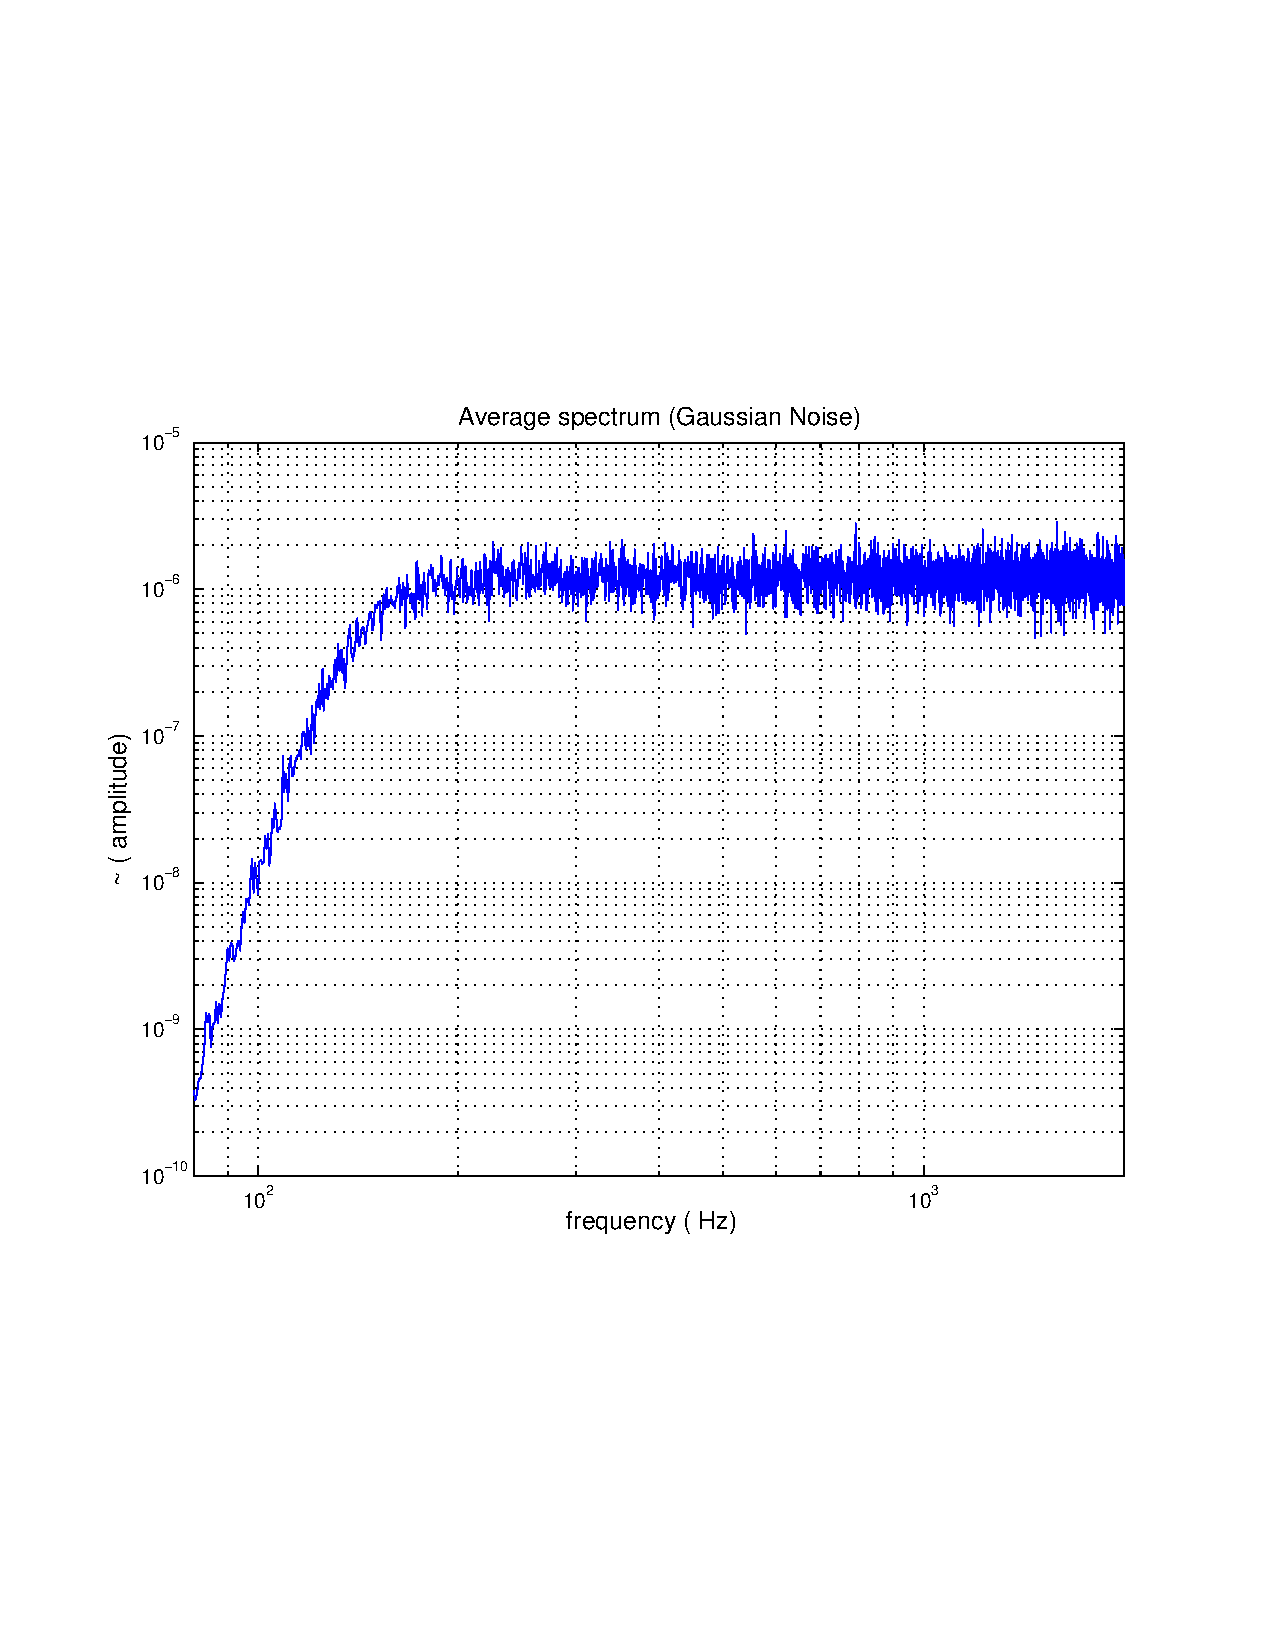
\includegraphics[width=0.9\textwidth]{figures/averagespec_psd}
\caption{Average Spectrum}
\label{fig:gaussianspectrum}
\end{center}
\end{figure}

\begin{figure}[h]
\begin{center}
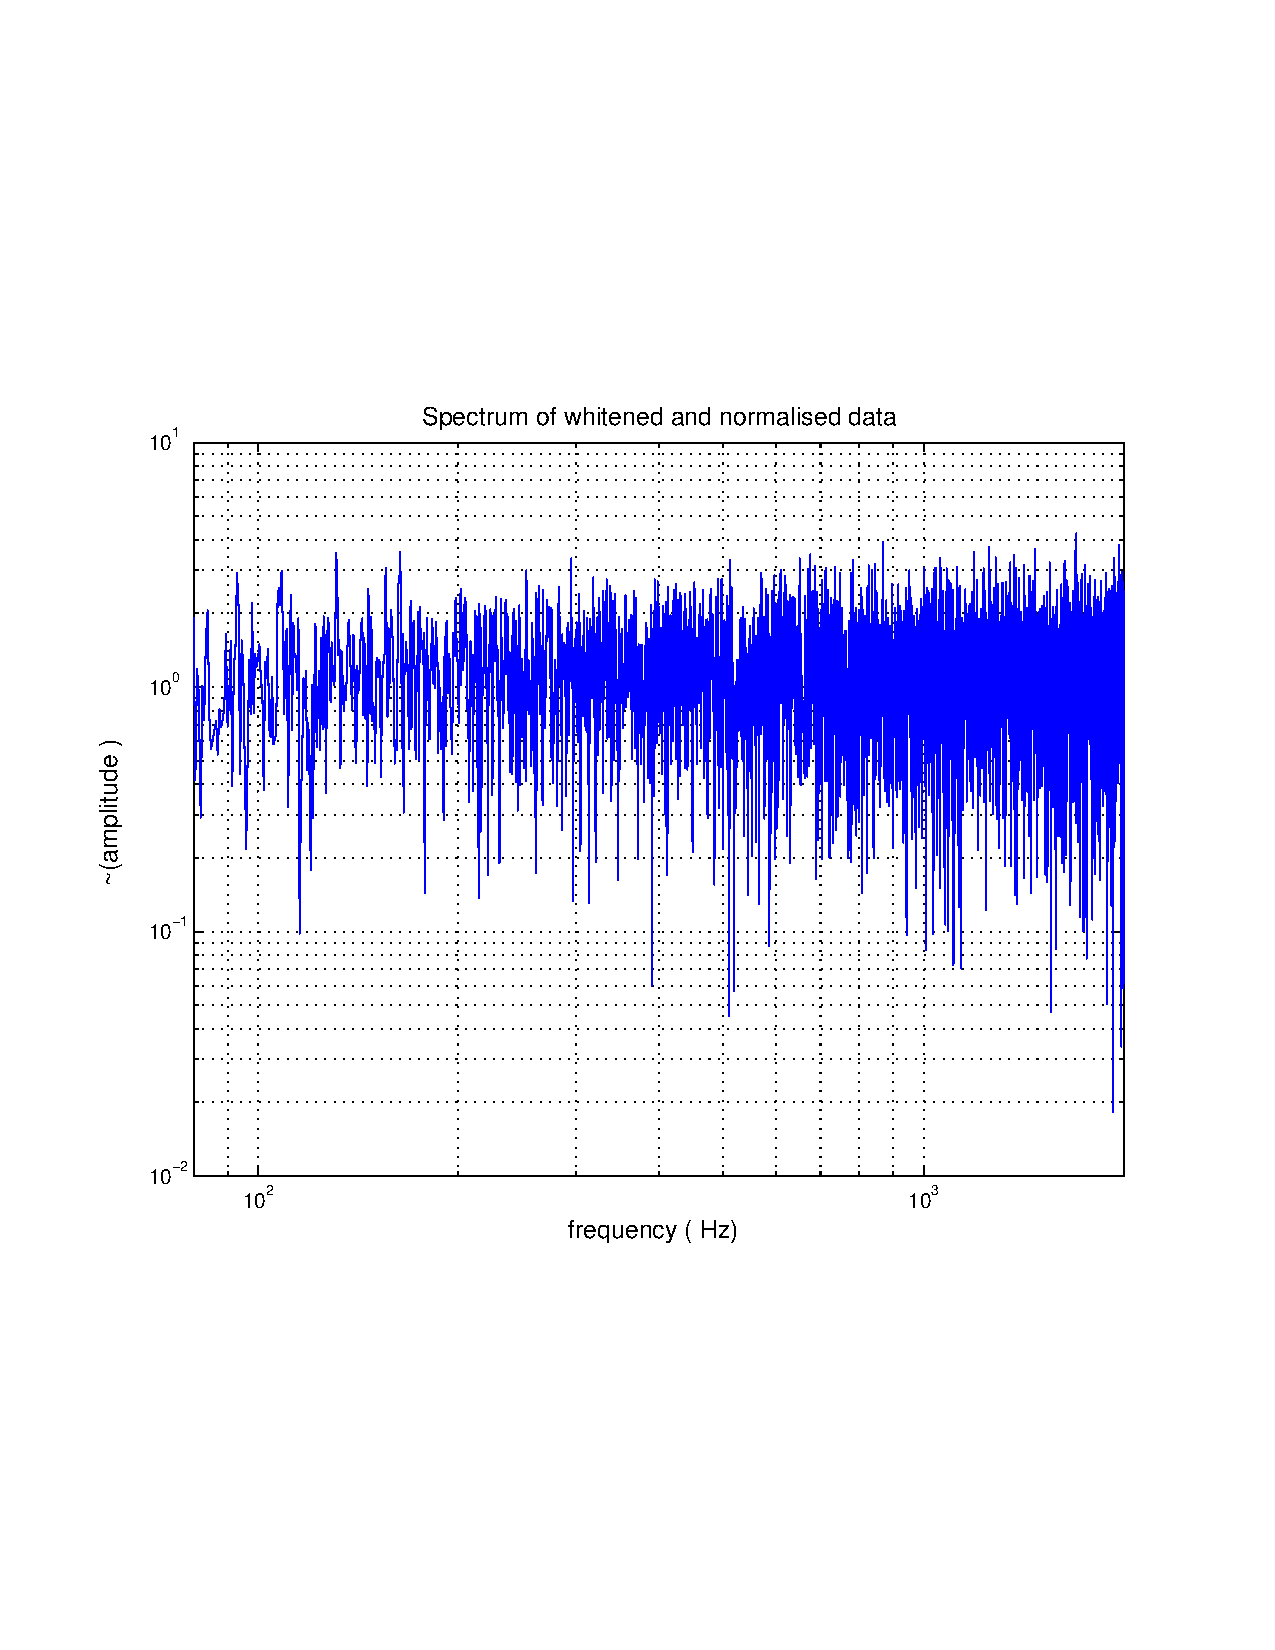
\includegraphics[width=0.9\textwidth]{figures/freqseries_psd}
\caption{Frequency series}
\label{fig:gaussianfreqseries}
\end{center}
\end{figure}
 
Our search method relies heavily on the fact that in Gaussian noise, 
 the power in a given tile is $\chi^2$-distributed with 
$2 V$ degrees of freedom where $V$ is the time-frequency volume of the 
tile(~\ref{chapter:powertools} ).  Hence to check if our measurements 
actually follow the right distribution we did the following:
\begin{itemize}
\item Selected a tile with degrees of freedom $dof_{\tau} = 2$ and $dof_{\tau} = 4$
\item Printed out the power in the tile from for each iteration.
\item Plotted the power distribution for these tiles and compared that to the plot
      of the theoretical $\chi^2$ distributed data with the corresponding degrees of freedom. 
\end{itemize}

Figure~\ref{fig:compchisquarenew} shows the result of our tests. 
The blue curve is the measured power distribution of the tiles with $dof_{\tau} = 2$ 
and the black curve is for $dof_{\tau} = 4$ while the green 
curve is the theoretical $\chi^2$ distribution with $2$ degrees of freedom
and the red curve is for $4$ degrees of freedom.  
\begin{figure}[h]
\begin{center}
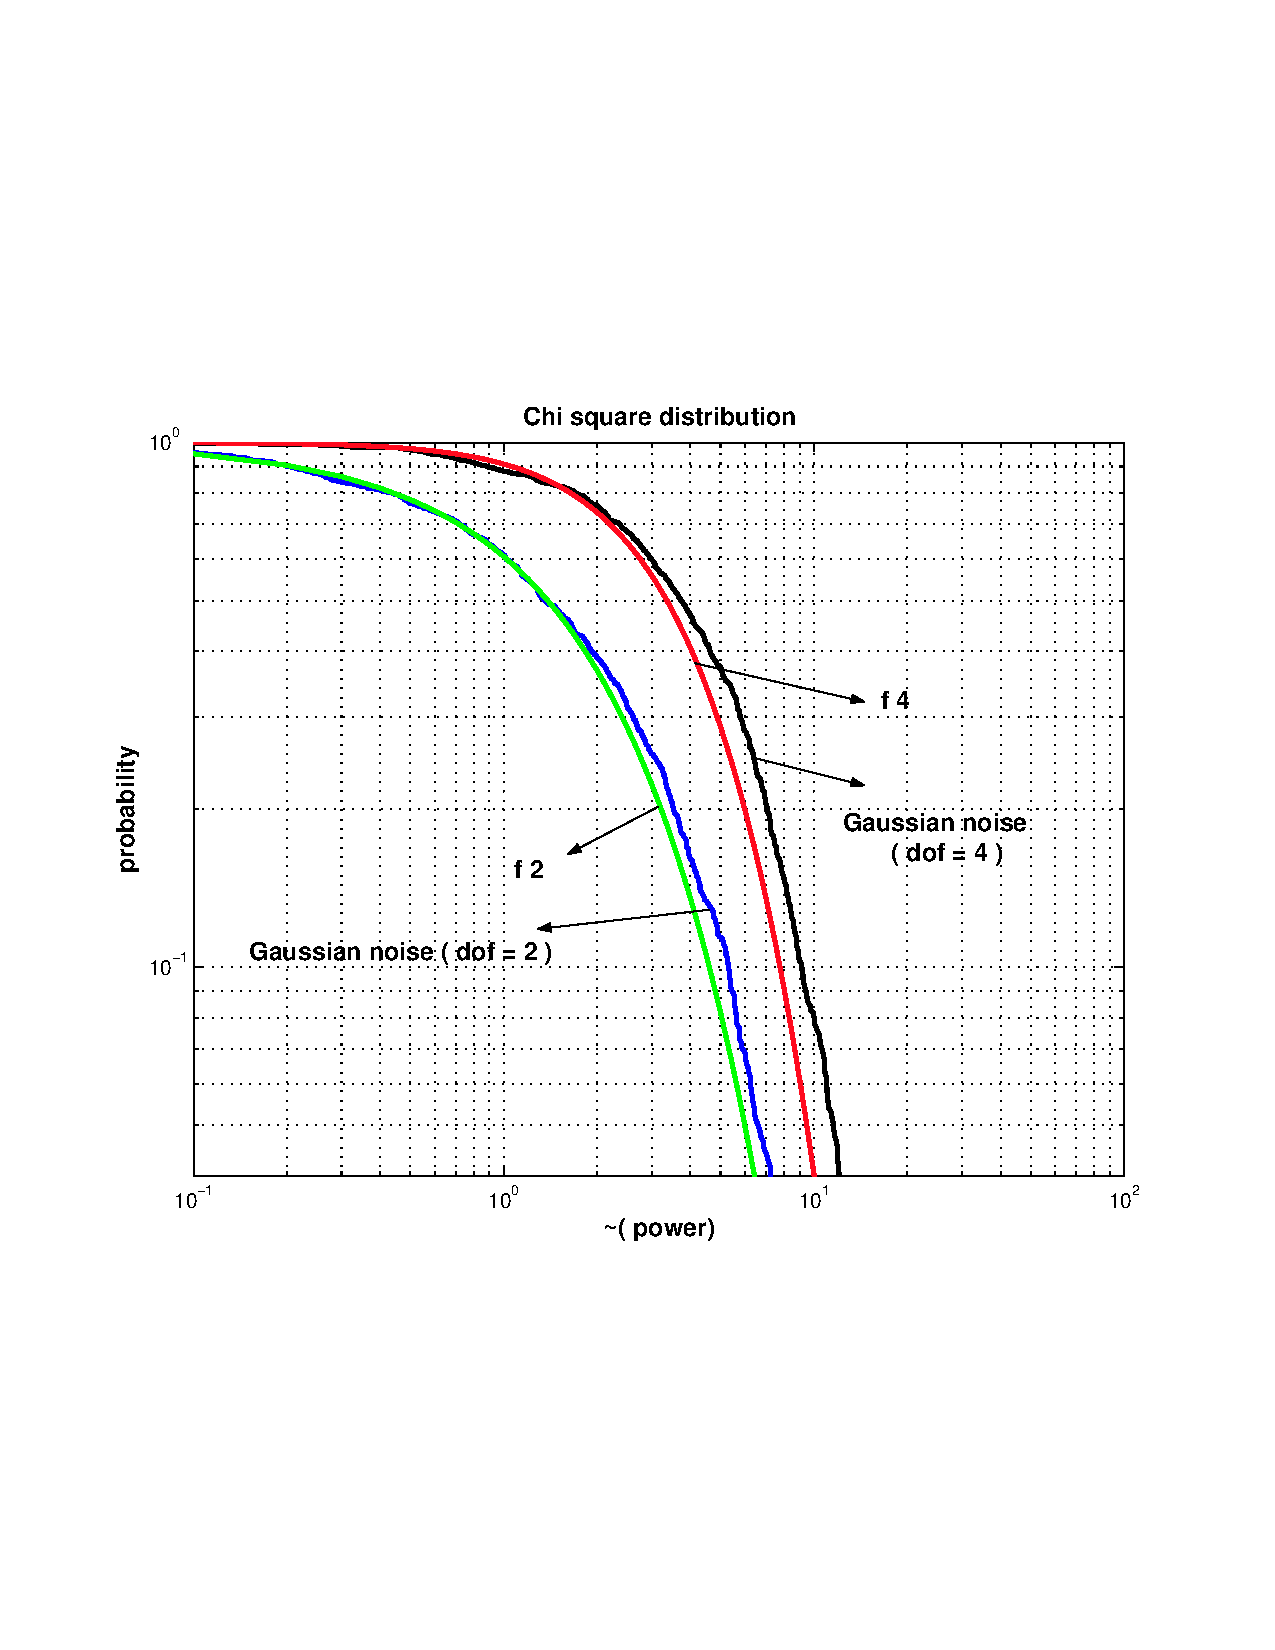
\includegraphics[width=0.9\textwidth]{figures/compchisquarenew2_4}
\caption{Comparison of the measured and theoretical distributions for the
  new time-frequency plane}
\label{fig:compchisquarenew}
\end{center}
\end{figure}     


\clearpage

\subsection{Butterworth Filter used in Excess Power Search}
\label{section:Butterworth}

The LIGO data is dominated by noise at low frequencies. We 
therefore apply a Butterworth high pass filter to get rid off these 
low frequency noise components. Here we report on a set of tests 
that were performed to check the performance of the high pass filter.

Of primary interest to us is the impulse response and frequency response 
of the filter. Figure~\ref{fig:checkbuttertimeseries} shows the 
time series containing a $\delta$ function before and after the 
application of the high pass filter:
\begin{figure}[h]
\begin{center}
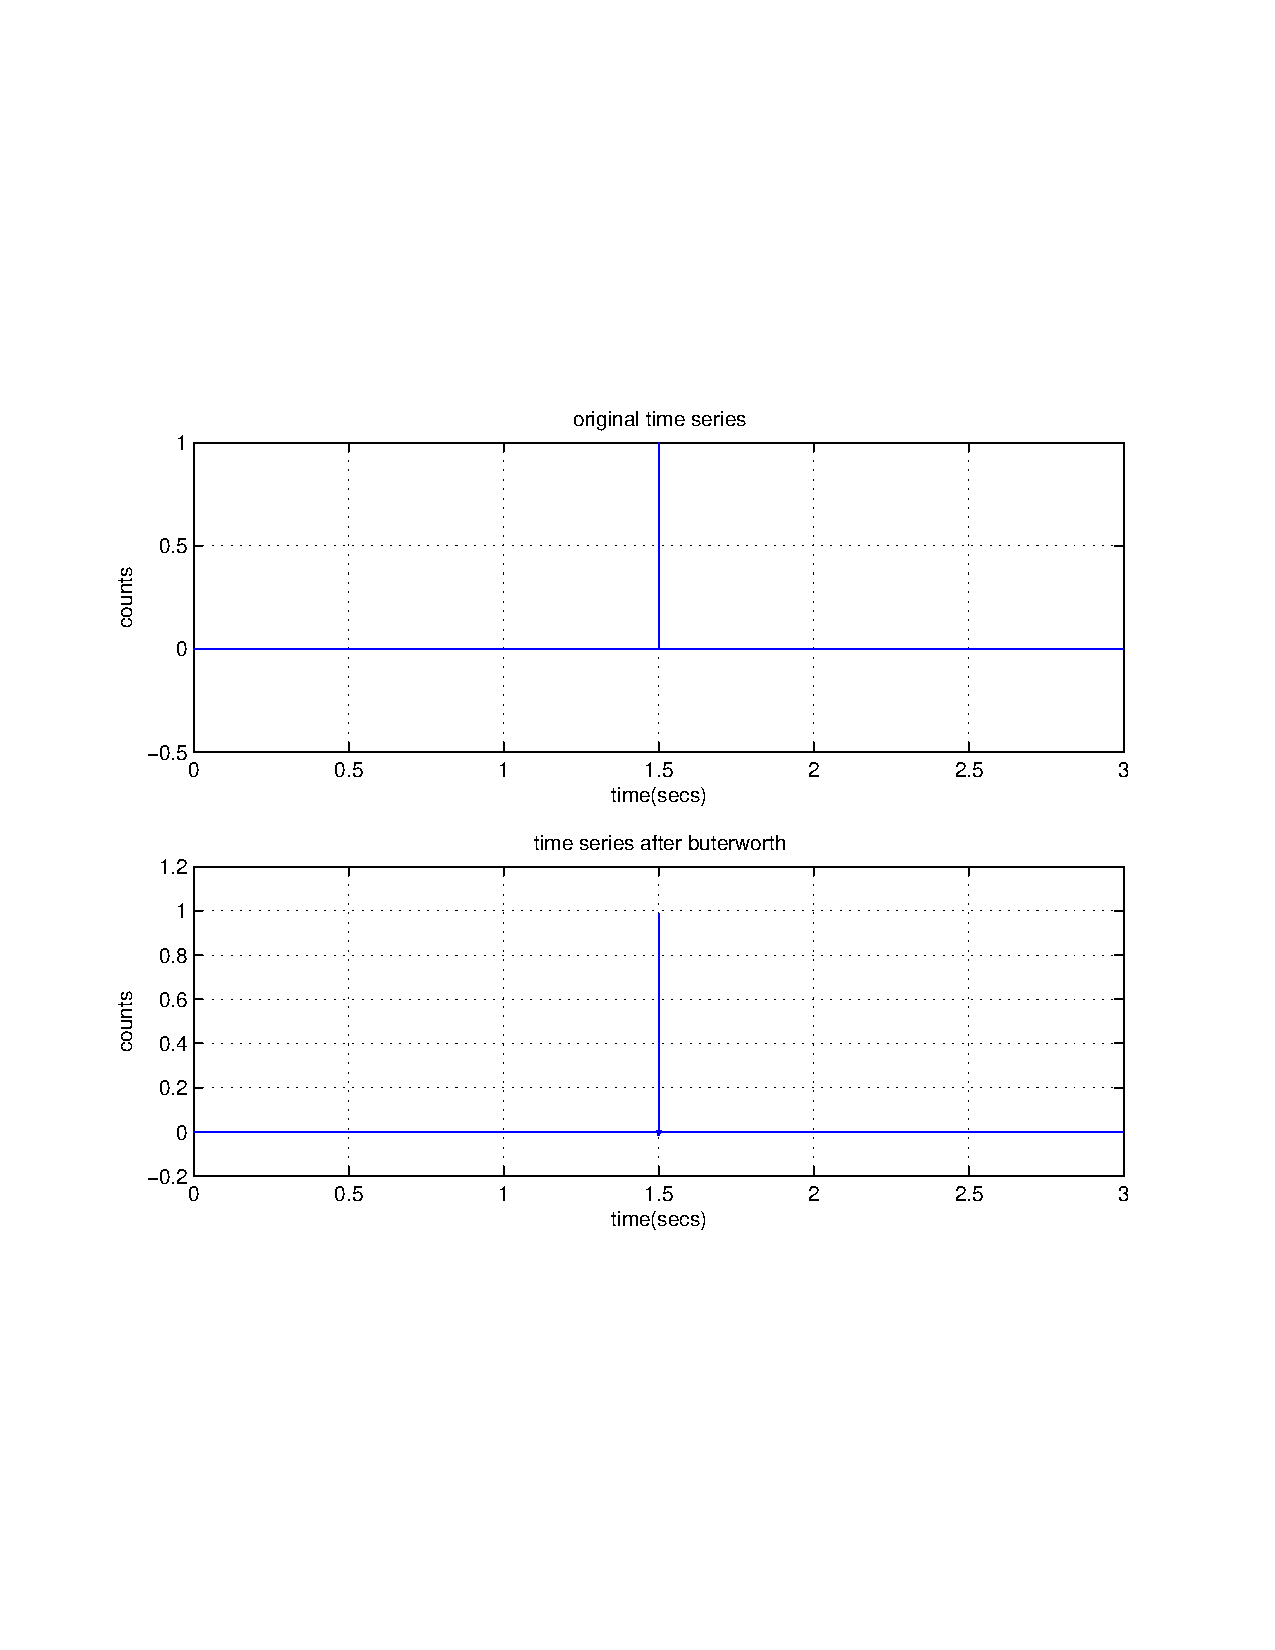
\includegraphics[width=0.9\textwidth]{figures/checkbuttertimeseries}
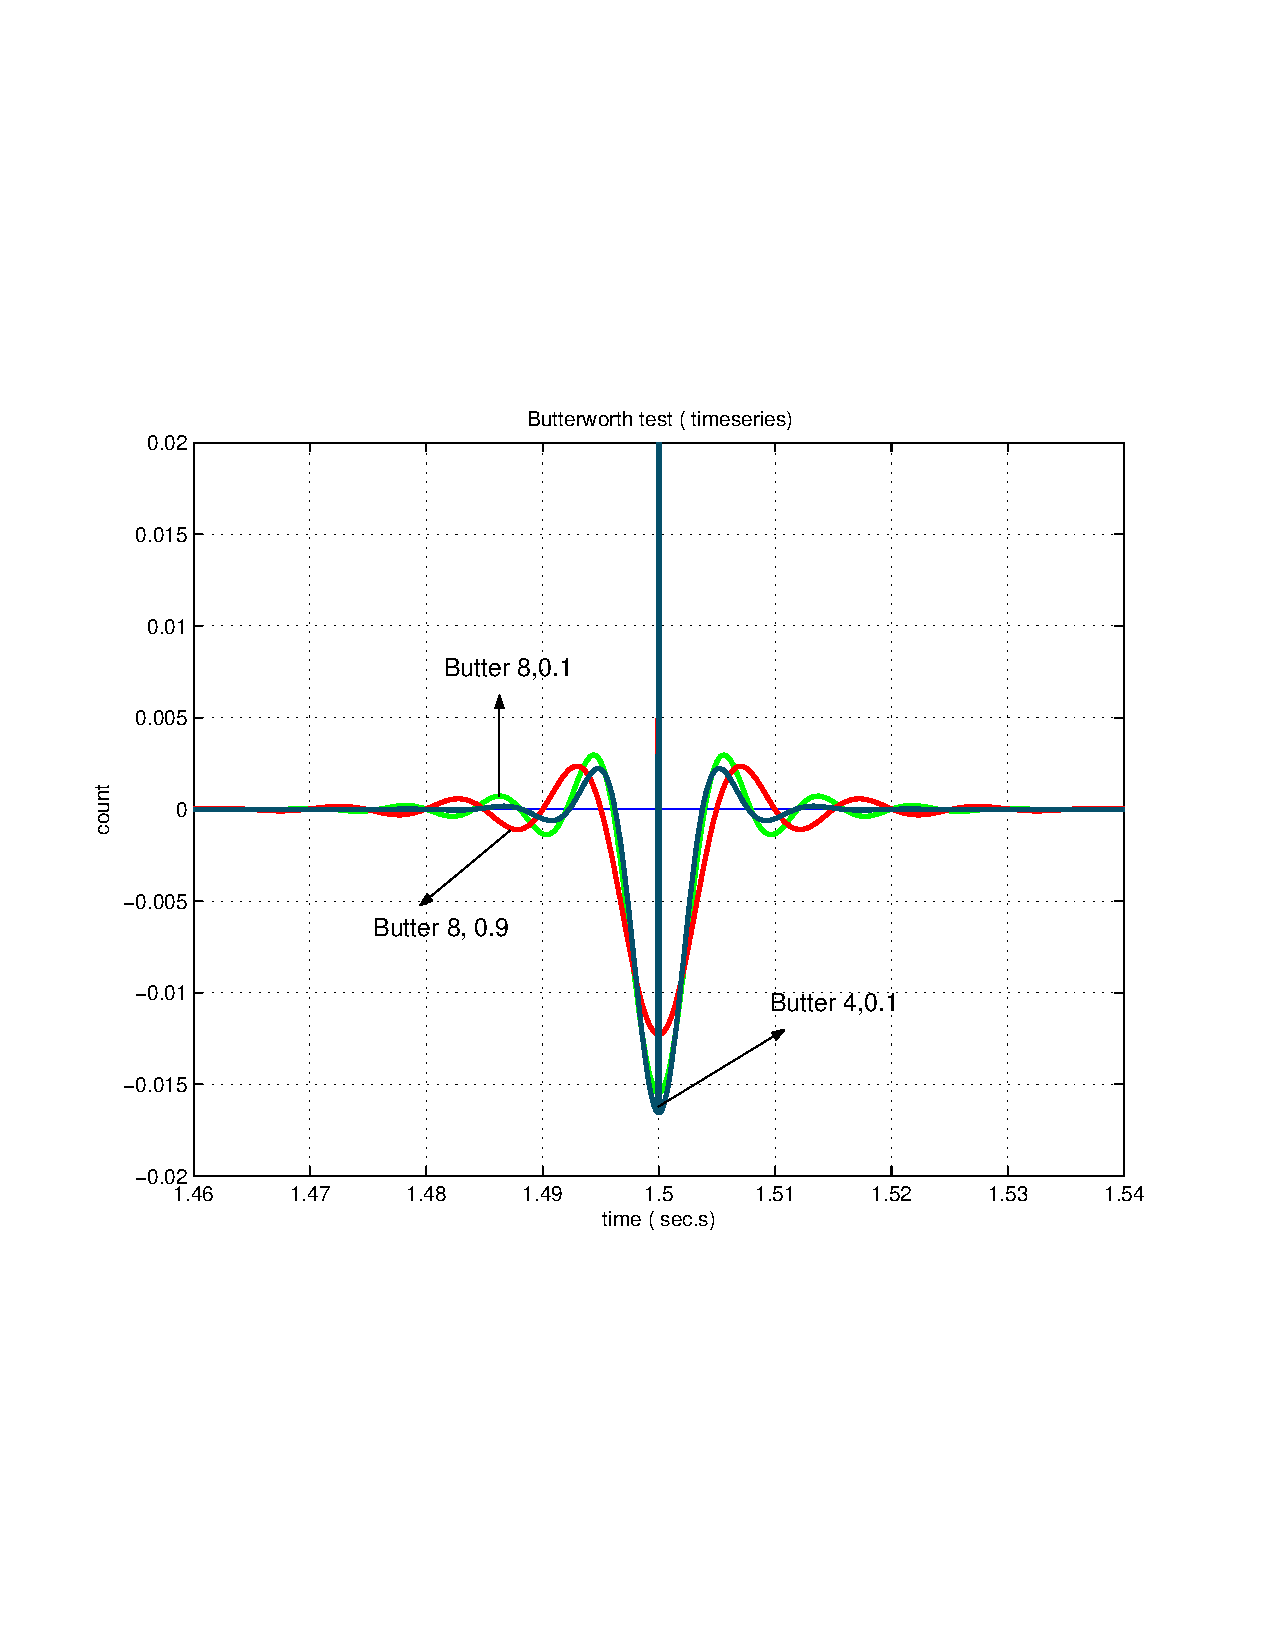
\includegraphics[width=0.9\textwidth]{figures/butter894comptimeseries}
\caption{Top panel: Time series before Butterworth and 
Bottom 2 panels: Time series after Butterworth} \label{fig:checkbuttertimeseries}
\end{center}
\end{figure}
The impulse response in Figure~\ref{fig:checkbuttertimeseries} shows  
time domain ringing produced by the filter. Maximum amplitude of 
the ringing is upto about $1.5$\% of the original time series amplitude.
However ringing in the side lobes die down to almost zero within about
20 milliseconds on both sides of the $\delta$ function. This ringing may
affect the timing resolution in real search, but we are yet
to quantify that effect.  

The Butterworth filter is created using the LAL routine,
\texttt{LALButterworthREAL4TimeSeries()} which uses the following 
parameters to specify the filter:
\begin{itemize}
  \item the low frequency cut off, f2. 
  \item The attenuation, a2. It gives a measure of power
    that is allowed to pass at f2.
  \item The filter order, nMax.
\end{itemize}

The frequency response of the filter is shown in Figure~\ref{fig:butterworthtest4} 
where the chosen parameters were $f2 = 120Hz$, $a2 = 0.1$ and $nMax = 4$.
\begin{figure}[h]
\centering
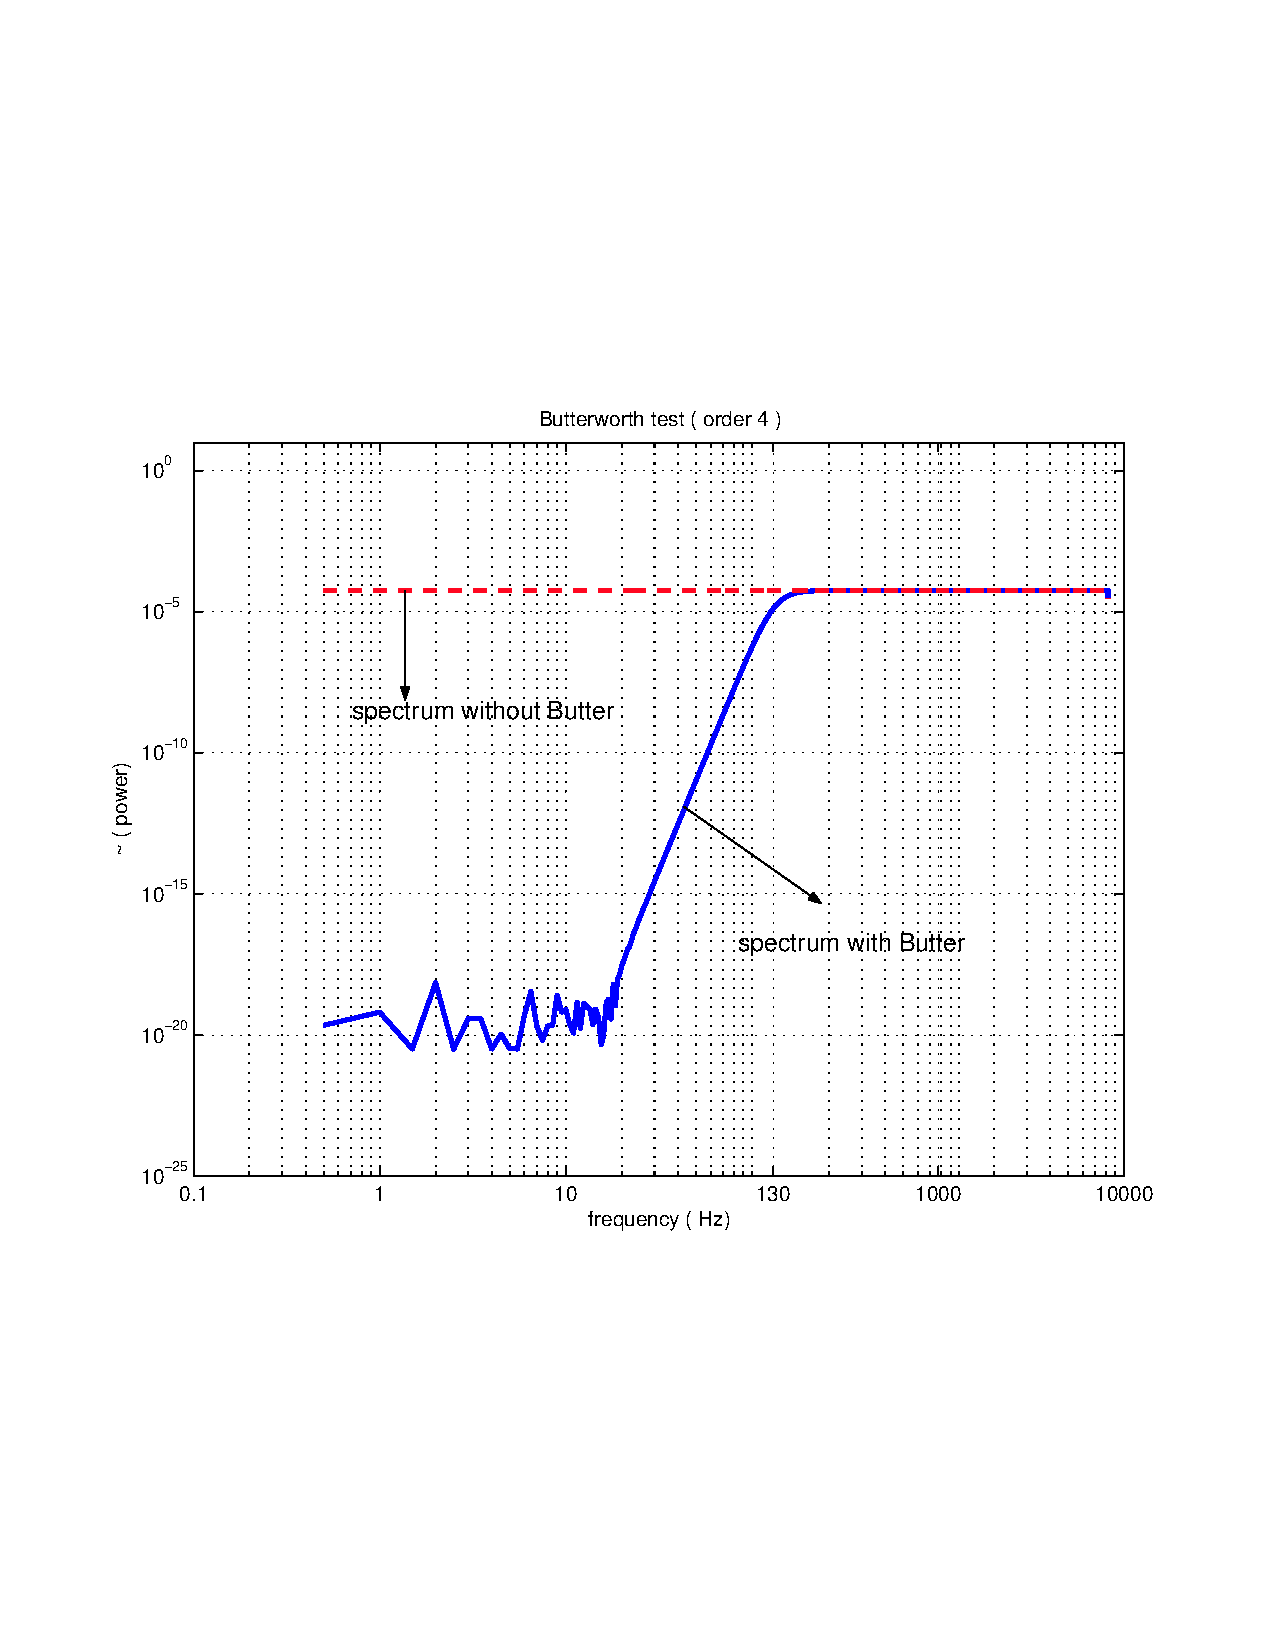
\includegraphics[width=0.9\textwidth]{figures/butterworthtest4}
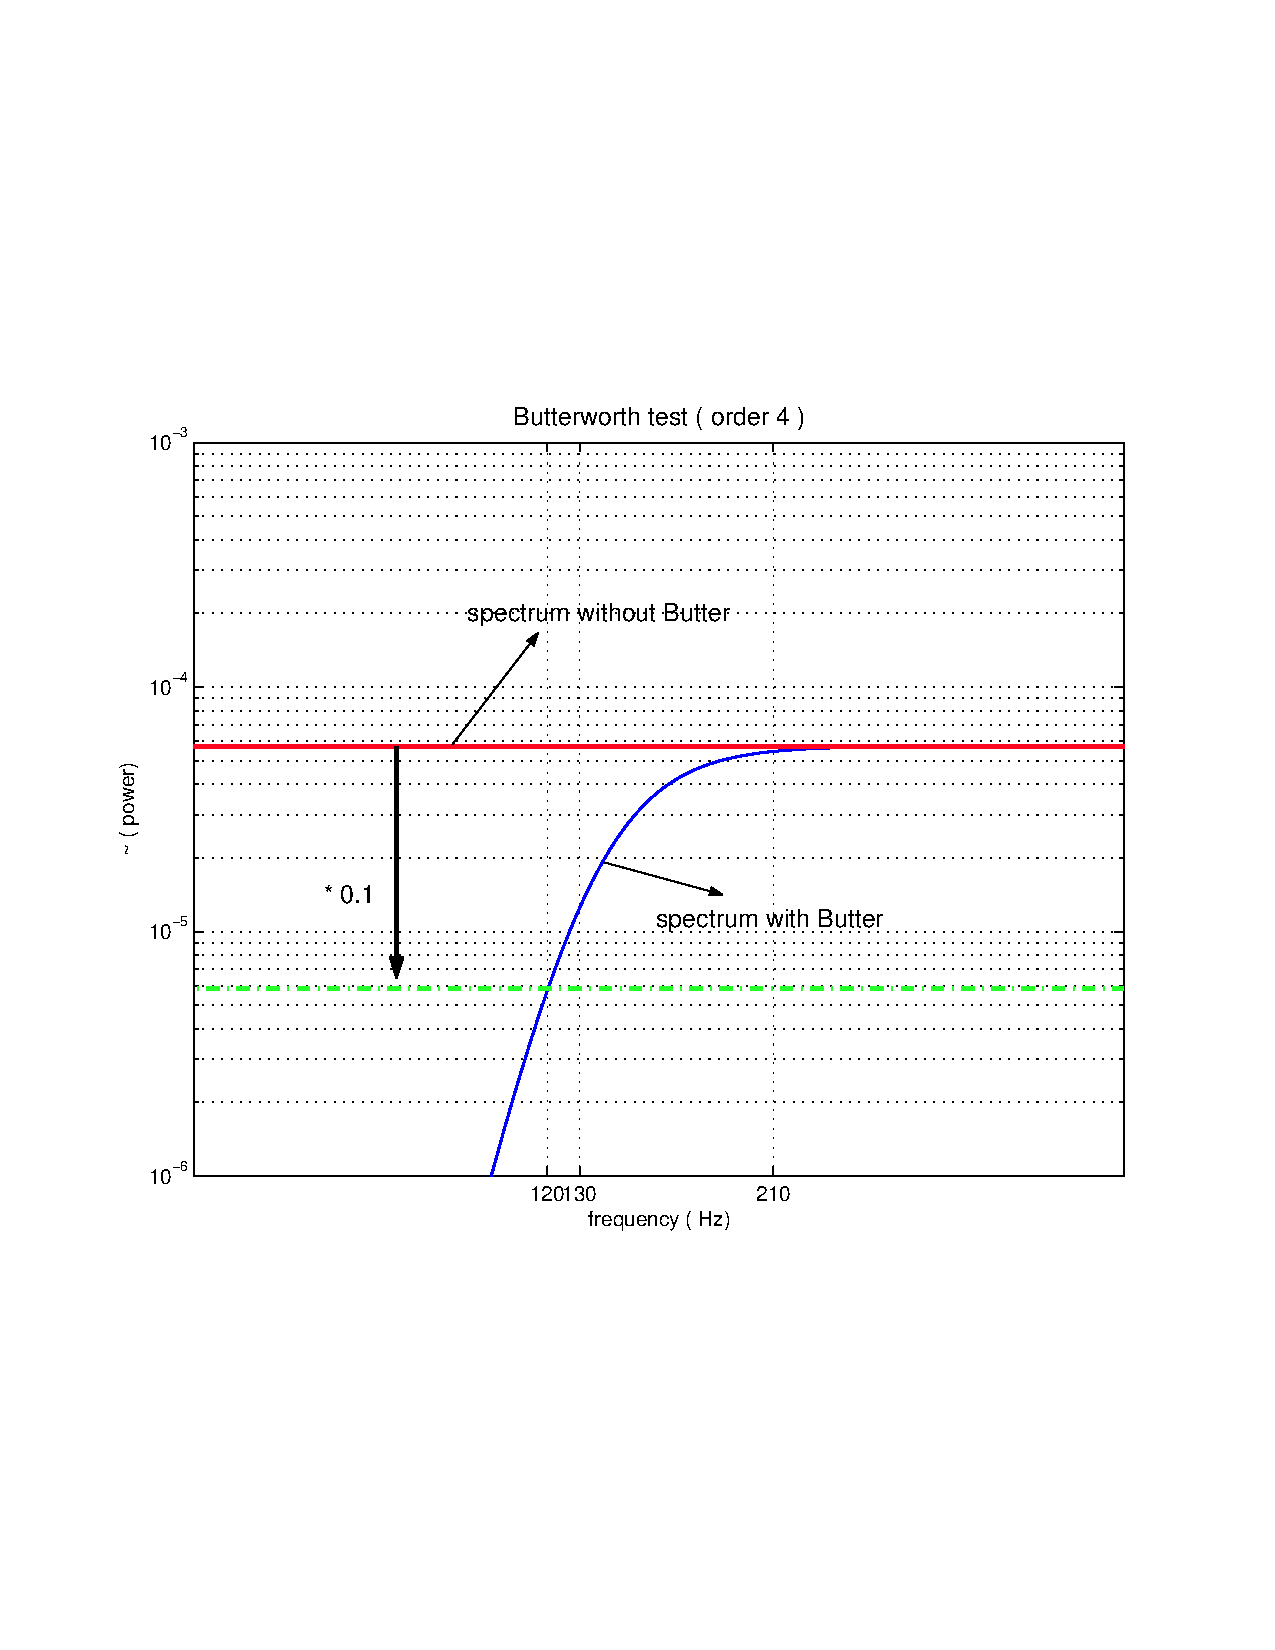
\includegraphics[width=0.9\textwidth]{figures/testattenuation4}
\caption{Frequency response of the high pass filter} \label{fig:butterworthtest4} 
\end{figure}
The red dotted line shows the spectrum which was measured without
the high pass filter while the blue line shows the spectrum after the data was 
high passed. From Figure~\ref{fig:butterworthtest4} 
it is evident that most of the frequency content below 100 Hz is being
blocked as desired. However this choice of parameters leeds to the 
undesirable feature that the signal power is suppressed all the way upto
$210$ Hz.                                         . 

The Excess Power code is configured to search for bursts above some 
minimal frequency, flow. It is therefore desirable to have little
or no attenuation above that frequency. The choice of Butterworth filter 
parameters that appear to achieve that are: 
\begin{itemize}
\item cutoff frequency,$f2 = flow - 10 Hz$
\item attenuatoin, $a2 = 0.9$
\item order, $Nmax = 8$
\end{itemize}
The frequency response of such a filter with $f2 = 120 Hz$ is shown in
Figure~\ref{fig:testattenuation8_9} 
\begin{figure}
\centering
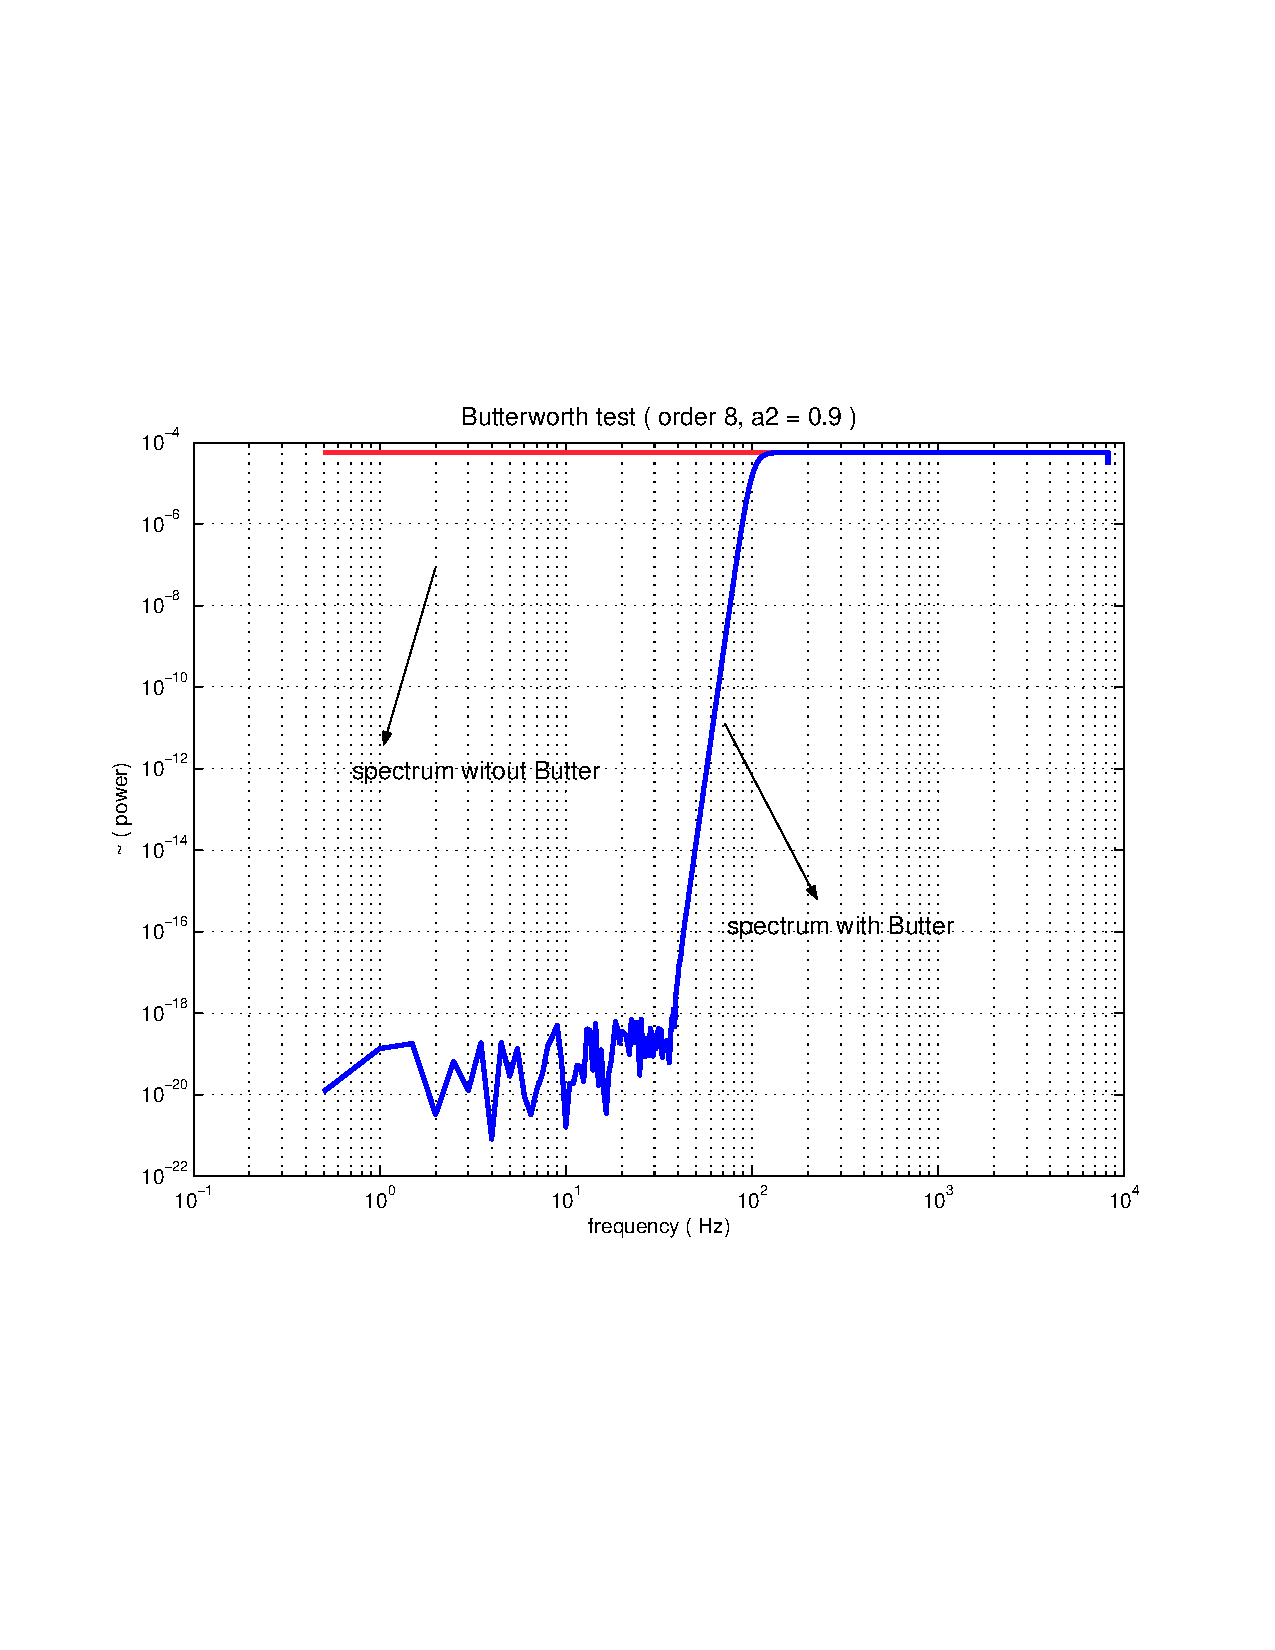
\includegraphics[width=0.9\textwidth]{figures/testattenuation8_9}
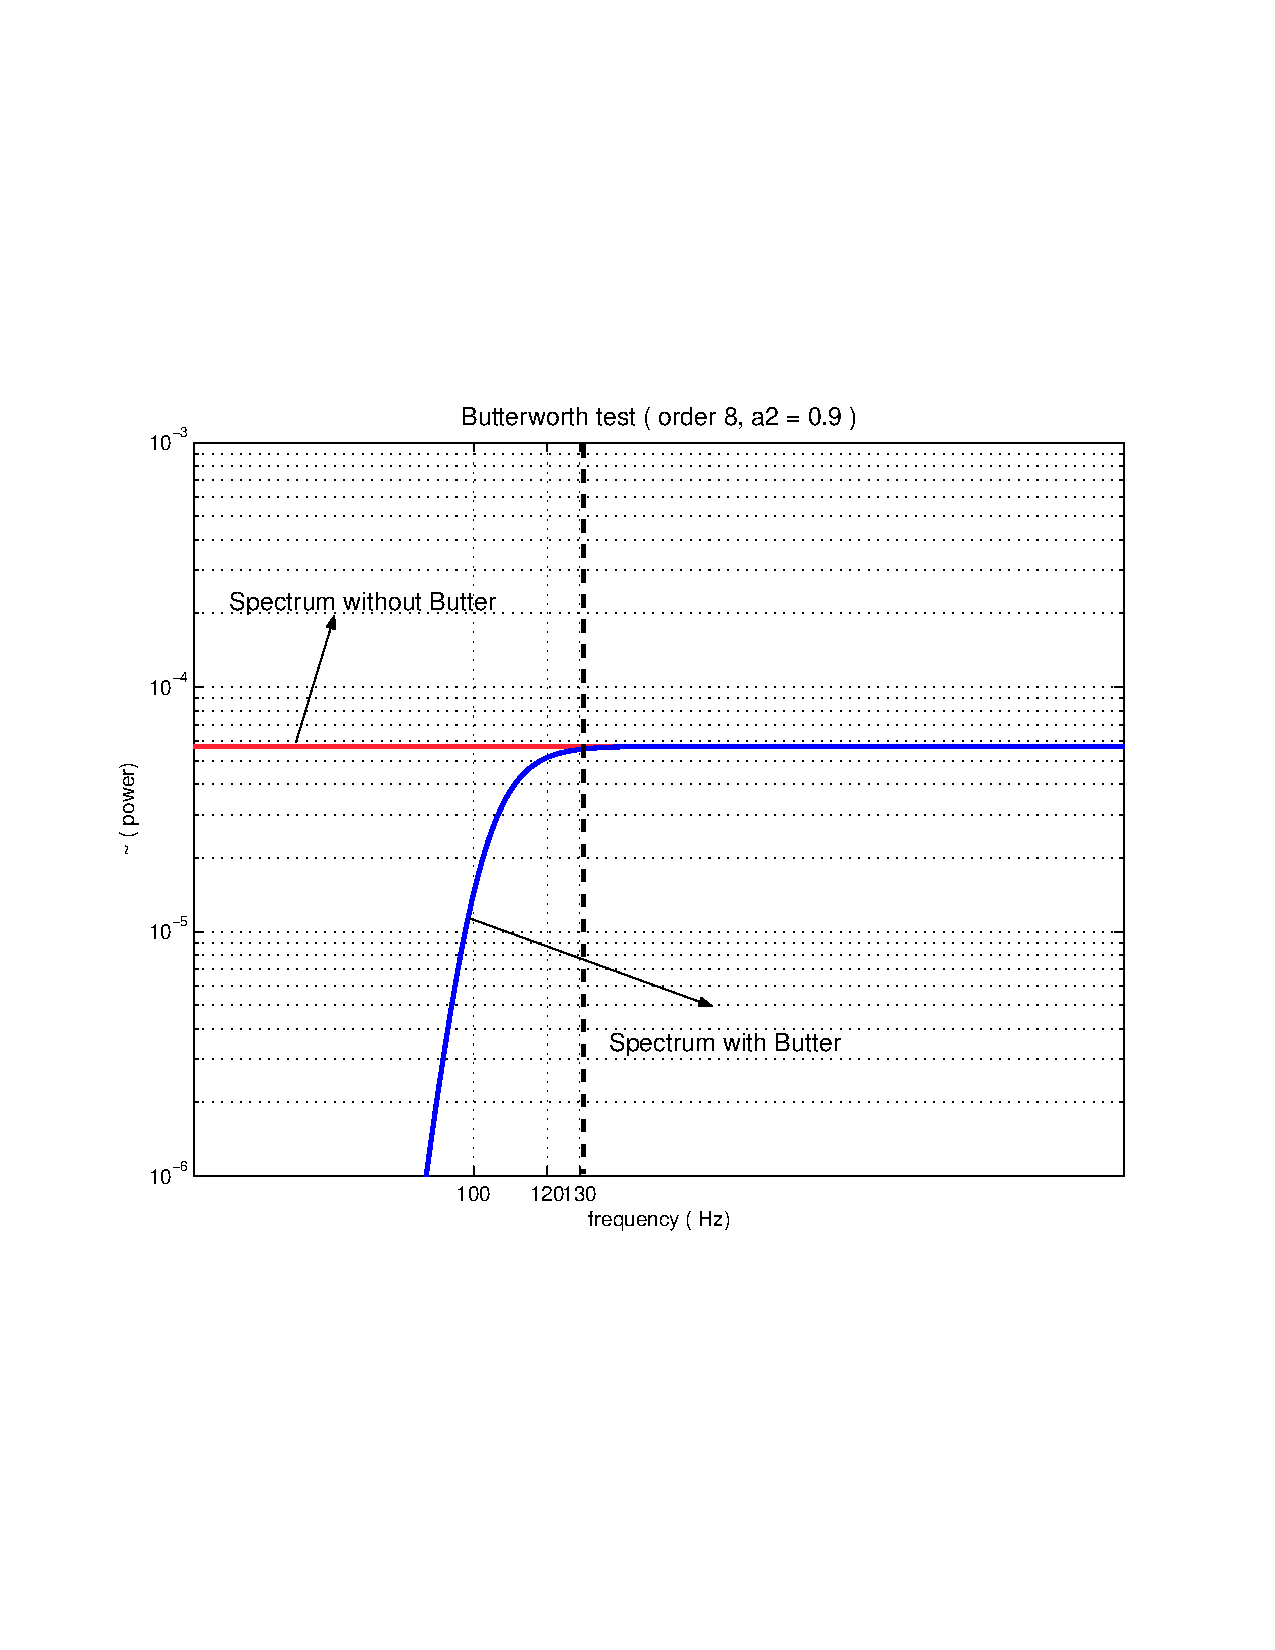
\includegraphics[width=0.9\textwidth]{figures/testattenuation8_9zoomed}
\caption{Comparison of the spectra: Filter order 8 and attenuation 0.9}
\label{fig:testattenuation8_9}
\end{figure}

\clearpage

\subsection{Clustering in Excess Power Search}
\label{section:clustering}

The excess power search is a multi-resolution analysis of the
time-frequency structure of the input time series.  A burst trigger is
identified if the probability of obtaining the excess power in a
time-frequency tile from Gaussian noise is smaller than some threshold
$\alpha$.   For large bursts in the data stream, many tiles can be
identified as triggers with different sizes and aspect ratios.   Hence when
the search over a particular segment is complete,   triggers have to be
clustered. 

The triggers are identified by a number of characteristic features like
start time,  peak time,  central frequency,  bandwidth,  excess power (the
excess compared to the power expected in Gaussian noise for the
corresponding time fequency volume)  and a confidence assosciated with this
measurement.  To do the clustering we first compare the peak times of the
triggers.  If the peak times are within an allowed range,  i.e. if
$|peaktime(trigger 1) - peaktime(trigger 2)| < dt$ where $dt$ is some
seconds,  we check whether the triggers  overlap in frequency.  If they
overlap,  we cluster them into one single trigger whose start time and
bandwidth are so chosen that they cover the time-frequency area which
includes the areas of the individual triggers.  The peak time of the
clustered trigger is equal to the peak time of that trigger which has more
excess power between the two.  Then we repeat the comparison but now
between the clustered trigger and another trigger.  If the peak times again
lie within the specified range and the frequencies overlap,  we modify,
otherwise we keep them as distinct triggers.  We repeat these steps until
there are no more distinct triggers which satisfy our criterion for
clustering.  The execess power of the cluster is the maximum of the
triggers involved in that particular cluster.

Top panel in Figure~\ref{fig:checkcluster}  shows a set of triggers before
clustering,  middle panel shows a set of clustered triggers when $dt$ was
chosen to be $10  nanosecs$ and the bottom panel shows the cluster when
$dt$ was $10  secs$. In the bottom panel there is only $1$ clustered
trigger and if one looks at the top panel this is expected because all the
peak  times of the triggers(before clustering)  lie within $10  secs$ of
each other.
\begin{figure}
\centering
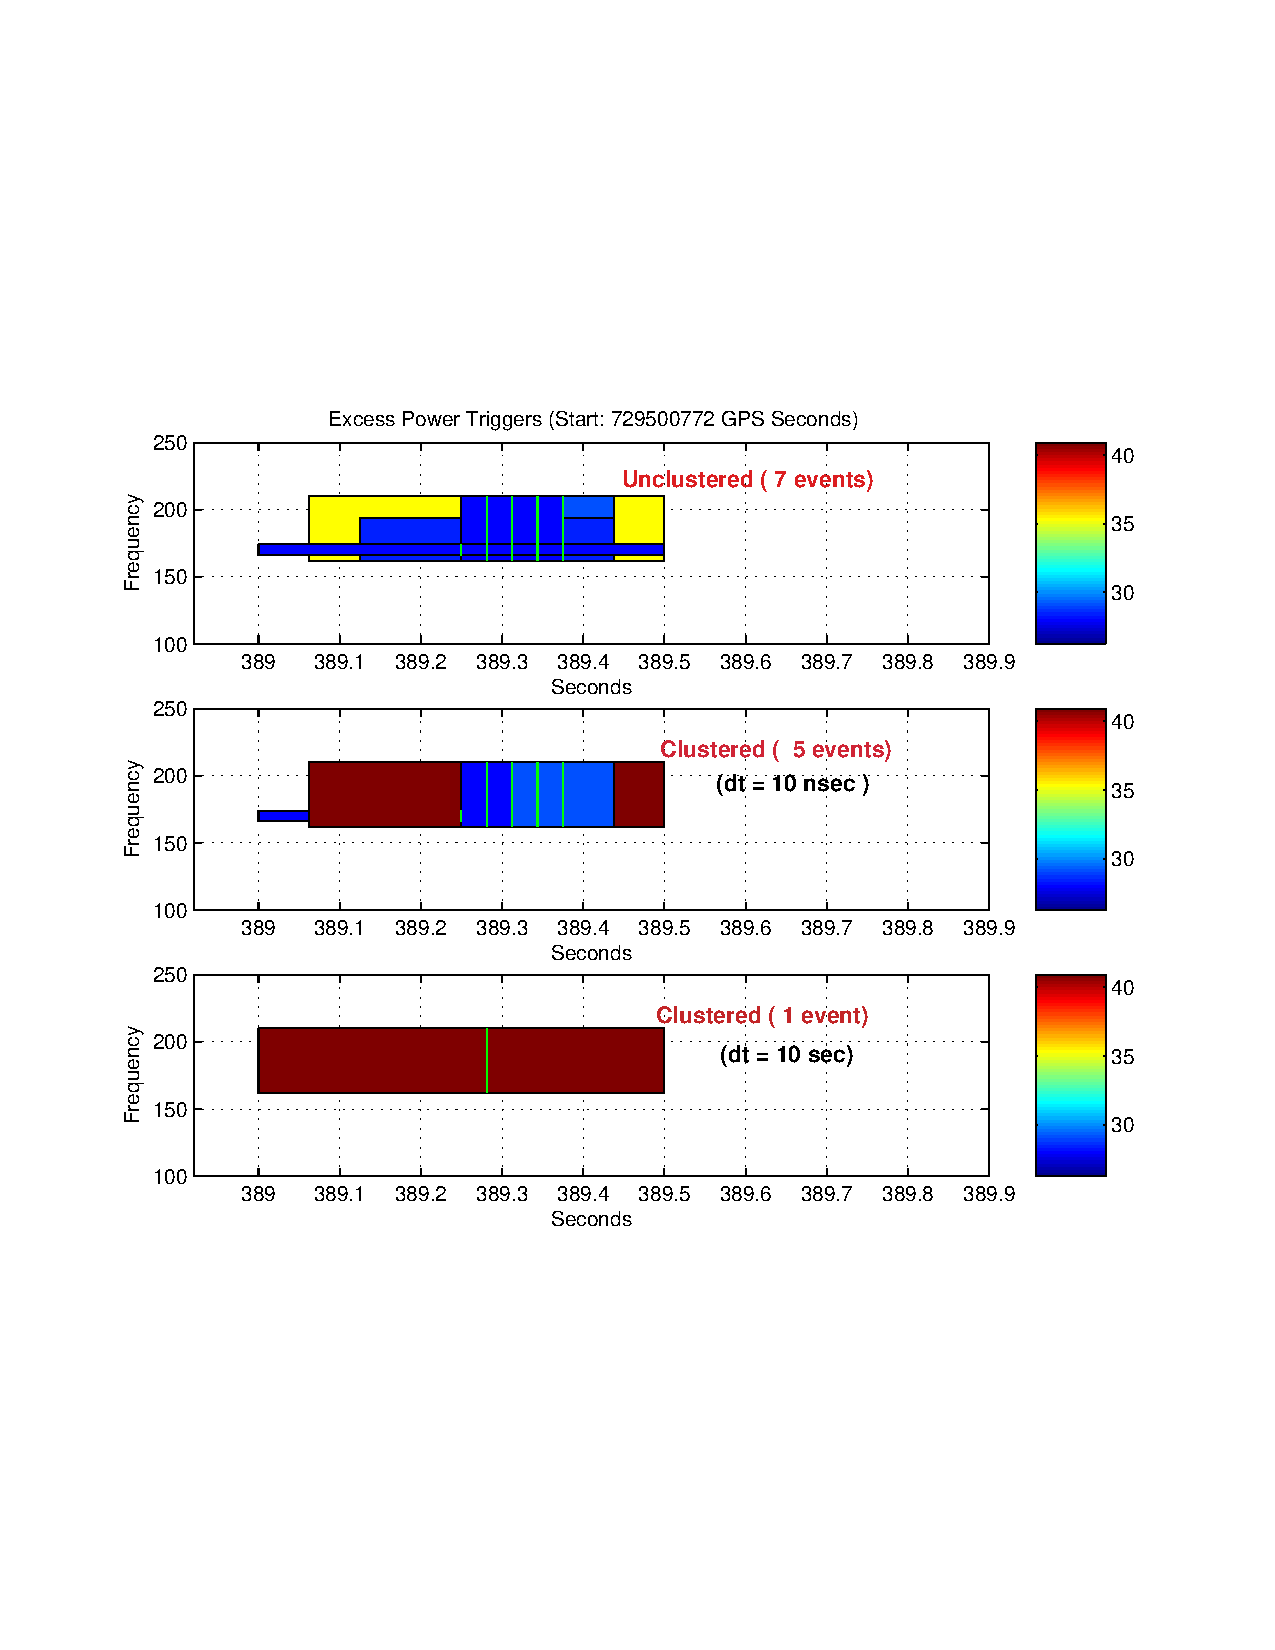
\includegraphics[width=1.0\textwidth]{figures/checkclustering_dt10nsec10sec}
\caption{Clustering in Excess Power}
\label{fig:checkcluster}
\end{figure}

To understand this better let us look at the triggers themselves:

\vspace{0.1 in}

\begin{tabular}{||l|l|l|l|l|l|l|lr||} \hline
no. & start time(sec) & peak time(sec) & duration(sec) & central freq(Hz) & bandwidth(Hz) & snr \\ \hline
1 &729501161.0  & 729501161.25  & 0.5     & 170  & 8   & 66.121277 \\ \hline
2 &729501161.125  & 729501161.28125  & 0.3125  & 186  & 48  & 123.3495 \\ \hline
3 &729501161.0625  & 729501161.28125  & 0.4375  & 186  & 48  & 120.2974 \\ \hline
4 &729501161.125 &729501161.28125 &0.3125 &178 &32 &82.274979 \\ \hline
5 &729501161.25 &729501161.3125 &0.125 &186 &48 &72.011459  \\ \hline
6 &729501161.25 &729501161.34375 &0.1875 &186 &48 & 92.914597 \\ \hline
7 &729501161.3125 &729501161.375 &0.125 & 186 &48 & 74.42984 \\ \hline
\end{tabular}

\vspace{0.1 in} 

The table above contains the set of triggers before clustering while   
the table below contains the $5$ clustered events when $dt$ 
was $10 nanosec$.

\vspace{0.1 in}

\begin{tabular}{||l|l|l|l|l|l|l|lr||} \hline
no. & start time(sec) & peak time(sec) & duration(sec) & central freq(Hz) & bandwidth(Hz) & snr \\ \hline
1 &729501161.0 &729501161.25 &0.5 &170 &8 & 66.121277 \\ \hline
2 &729501161.0625 &729501161.28125 &0.4375 &186 &48 &123.3495 \\ \hline
3 &729501161.25 &729501161.34375 &0.1875 &186 &48 &92.914597 \\ \hline
4 &729501161.25 &729501161.3125 &0.125 &186 &48 &72.011459 \\ \hline
5 &729501161.3125 &729501161.375 &0.125 &186 &48 &74.42984 \\ \hline 
\end{tabular}

\vspace{0.1 in}

Thus from this set of clustered triggers it is quite clear what we have been 
discussing till now.

\clearpage

\subsection{Tuning the excess power pipeline}
\label{section:tuning}

The excess power search identifies time-frequency tiles as events when the 
probability of getting power in the tile from Gaussian noise alone
is below some particular threshold.  The search assumes no particular 
information about the gravitational wave signals other than the time
frequency ranges to search for,  so once those ranges are chosen the main 
tool to tune the pipeline is by tweaking the threshold.  The other parameter 
to test in the tuning procedure is the coincidence window.  Thus to 
summarize the parameters to tune in the excess power search are:
\begin{itemize}
\item maximum duration(seconds) of the tiles
\item maximum bandwidth of the tiles
\item probability thresholds on the individual instruments
\item the coincidence window
\end{itemize}
In the following sections we will go over the tuning of the different 
parameters in more details.

\subsubsection{Tuning the size of the tiles}
\label{section:tunetilesize}

The size(duration and bandwidth) of the tiles are largely guided by the
time-frequency content of the gravitational waves one is searching for.
  Here,  we describe the tuning procedure where we were concentrating 
on the search of the merger phase preceded by an inspiral phase.  As
mentioned before the physical parameters describing the merger phase
of a binary black hole coalescence are very poorly understood till
today.  However there are some rough estimates available in the literature 
which we will briefly describe here.  These will provide us a guideline
in choosing the parameters of our search pipeline. [FH:Flannagan and Hughes]

The process of coalescence can be roughly divided into three phases:
\begin{itemize}
\item Inspiral phase
\item Merger phase
\item Ringdown phase
\end{itemize}
The inspiral phase can be modelled accurately enough to use the match
filtering techniques to search for the waveforms, however for massive
black holes when there are not enough cycles left in the inspiral phase 
we have to rely on the merger phase for the detection of the coalescence.
According to the estimates of FH, binary black hole systems with total
mass $M \leq 30M_{\odot}$ are best searched for via their inspiral waves
while systems with $M > 30M_{\odot}$ must be searched via their
merger waves and/or their well understood ringdown waves.  


FH has estimated a conservative value for the merger frequency given
by 
\begin{equation}
f_{merge} = \frac{0.02}{M} \\
          = 205 Hz (\frac{20M_{\odot}}{M})
\label{eq:fmerge}
\end{equation}.
This is conservative in the sense that one can reasonably be sure that
numerically generated templates will not be needed before $f = f_{merger}$.
Now LIGO noise floor restricts the lowest frequency that can be searched 
for and in $S4$ this is $\approx 50 Hz$. Using Eq~\ref{eq:fmerge} we 
then get that a binary system of maximum mass $\approx 80M_{\odot}$ 
can be searched for in $S4$.  However for a $80 M_{\odot}$ binary the 
number of cycles in the inspiral phase will be very small and since we
are interested in the coincidence of the mergers with the inspirals we
would like to restrict our search to a bit lower total mass.  Thus the 
mass range of the binary black holes that we decide to look at for the 
IB search is given by 
\begin{equation}
30 M_{\odot} < M \leq 70 M_{\odot}. 
\label{eq:massrange}
\end{equation}
Given this mass range let us now see what can we estimate about the 
expected frequency and duration of the merger signals. From 
Eq~\ref{eq:fmerge} we get the approximte range of the merger frequencies:
\begin{equation}
58 Hz < f_{merge} \leq 140 Hz
\label{eq:frange}
\end{equation}
Now according to FH the high frequency shut off for the mergers are
roughly given by 
\begin{equation}
f_{qnr} = 1320 Hz (\frac{20M_{\odot}}{M})
\label{eq:fqnr}
\end{equation}
Thus if the assumed bandwidth of the merger signal is 
$\Delta f = f_{qnr} - f_{merge}$,  then for our mass range of 
interest we may expect the bandwidth to be of the order of few
hundred Hertz.  

The effective duration for the signals has also been roughly estimated
by FH to be:
\begin{equation}
50 M < T < 10 M
\label{eq:timerange}
\end{equation}
depending on the total spin of the binary system. If we consider
a coalescence where both the inspiraling black holes are nearly
maximally spinning, with their spins and the orbital angular momentum
nearly alligned then the merger may be expected to be long,  while
for non-spinning black holes the merger will be rather quick.  Thus 
given our mass range of interest (Eq~\ref{eq:massrange}) the 
time duration of the expected signals whould be somewhere in the 
range:
\begin{equation}
17.2 ms < T < 1.5 ms
\label{eq:trange}
\end{equation} 
  
So given these estimates about the bandwidth and the duration of the 
signals of our main interest we choose the following parameters in our
search pipeline:
\begin{itemize}
\item Low frequency cutoff: $50 Hz$
\item Bandwidth: $1024 Hz$
\item Maximum duration of a tile: $125 ms$; we have set the duration 
a few times longer than the maximum duration in Eq~\ref{eq:trange}
because of the uncertainty in the estimations related to the nature 
of the merger signals.
\item Maximum bandwidth of a tile: $128 Hz$; we have the bandwidth 
smaller than the estimated bandwidths for the merger signals since
because of the LIGO noise curve the prominent contribution to the 
power from the merger phase will be for a few hundred Hertz.
\end{itemize}
The last two parameters set the maximum duration and bandwith of 
a single tile in the search,  which does not preclude us from searching
for longer or broader signals since we can always sum up the power
from multiple tiles triggered by the particular signal. 
    
\subsubsection{Deciding on the probability thresholds}
\label{section:tunethreshold}
We saw in Sec~\ref{section:tunetilesize} that the sizes of the tiles
are mainly guided by the rough expectations about the signals that 
we are interested in.  However, the threshold on the probability
of power in a tile is guided by the optimisation between the false 
rate and efficiency to a set of Monte Carlo simulations.  The idea
we usually follow is to choose a threshold which lowers the false rate 
maintaining the efficiency at an acceptable value.

To get a rough idea about the region where we start loosing significant 
amount of efficiency without an appreciable effect in lowering the false 
rate we estimate the efficiencies and the false rates for a number of 
thresholds. We have used $Q9$ Sine-Gaussian waveforms at $235 Hz $ to
perform the tuning and the confidence thresholds are
$\{-30.0, -35.0, -40.0, -45.0, -50.0, -55.0, -60.0, -65.0, -70.0, -80.0, 
-90.0, -100.0, -150.0, -200.0\}$. How the efficiency and the false rate 
depend on the thresholds are shown in Fig~\ref{fig:dt125df128tune}: 
\begin{figure}[h]
\begin{center}
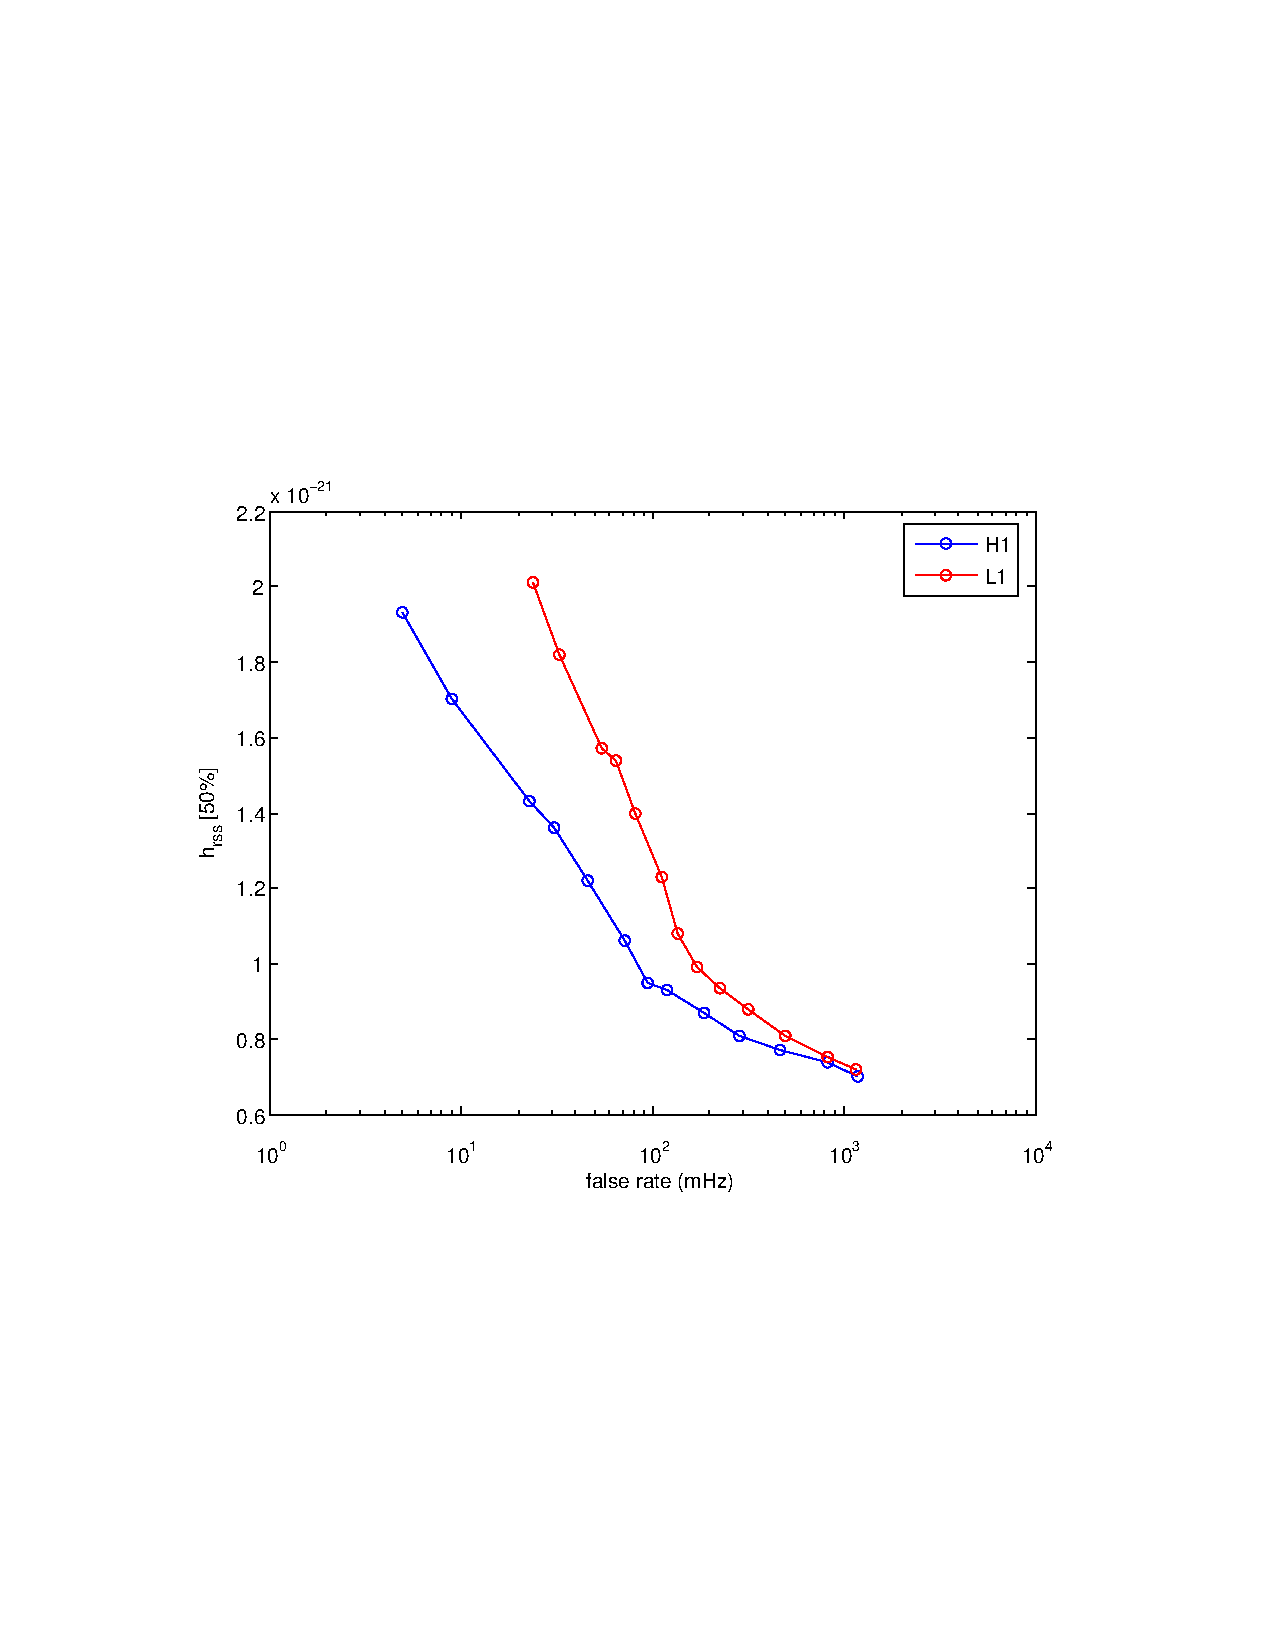
\includegraphics[width=1.0\textwidth]{figures/H1_L1_dt125_df128}
\caption{Efficiency vs. False rate for different |thresholds|}
\label{fig:dt125df128tune}
\end{center}
\end{figure}
The circles on the curves show the values corresponding to different 
thresholds.  The maximum false rate and the best efficiency are obtained 
for the lowest |threshold|(30.0),  then as the |threshold| is increased
the false rate decreases while the efficiency gets worse. Around the 
|thresholds| of $50.0 - 60.0$ one may notice that for a very small 
decrease in false rate the efficiency gets a whole lot worse.  This gives 
us a rough idea that we should choose $ |threshold| < 60.0$.  However
one should be aware of the fact that tuning must be specific to the 
pipeline being run.  In our pipeline we have a coincidence step which
involves the burst triggers and the inspiral triggers and we are not
quite sure how many of the false triggers will survive that step. We
also plan to use the Hanford 2Km instrument in a coherent follow up at
the end of the pipeline which will also hopefully get rid off many of the
false triggers. However we would like to  
have a good estimate of the background distribution of triggers and so 
have a few surviviors at the end of the pipeline.  Keeping that 
in mind we decided to choose a looser threshold on the confidence 
probabilities. The thresholds we chose are 
\begin{itemize}
\item Threshold on H1: -38.0
\item Threshold on L1: -38.0; The instrument in Livingstone was less 
sensitive than the one in Hanford for the first half of the run but 
for the second half both the instruments had equal sensitivity.  So
we decided to have the same thresholds on both the instruments.
\end{itemize}      
These thresholds were so chosen so that the false rate after 
coincidence between H1 and L1 triggers is $\approx 0.2 mHz$ while 
the $ h_{rss}$ is $\approx 1.12e-21$.

\subsubsection{Choosing the coincidence window(W)}
\label{section:tunewindow}
The coincidence window(W) is given in milliseconds(ms).  When we 
have a trigger and want to find if there are triggers in the 
other instrument which are 
coincident with that we first pick the triggers which are within
$+/- W ms$ of the peak time of that trigger.  Once we find such a 
trigger we compare the time duration and frequency bandwidths and
if they overlap we mark them as coincident triggers. Ideally if a trigger 
is caused by a real gravitational wave signal then we expect that the
signal will trigger in the other instrument within $\approx +/- 10 ms$
since the light travel time between the two sites is that. But in the 
real analysis we may at times have to set longer windows because of 
errors creeping in from different sources like the timing inaccuracies 
of the search algorithm, errors in calibrations, etc..  In this step 
we choose the coincidence window for our pipeline.

We decided to choose the right window by doing a number of experiments
in the sense that we estimated the false rates and efficiencies
for a number of window sizes: $\{400 ms, 300ms, 200ms, 150 ms, 130ms,
110ms, 90ms, 70ms, 50ms, 30ms, 15ms\} $.  Fig~\ref{fig:tuneburcawindow}
shows the results of that experiment:   
\begin{figure}[h]
\begin{center}
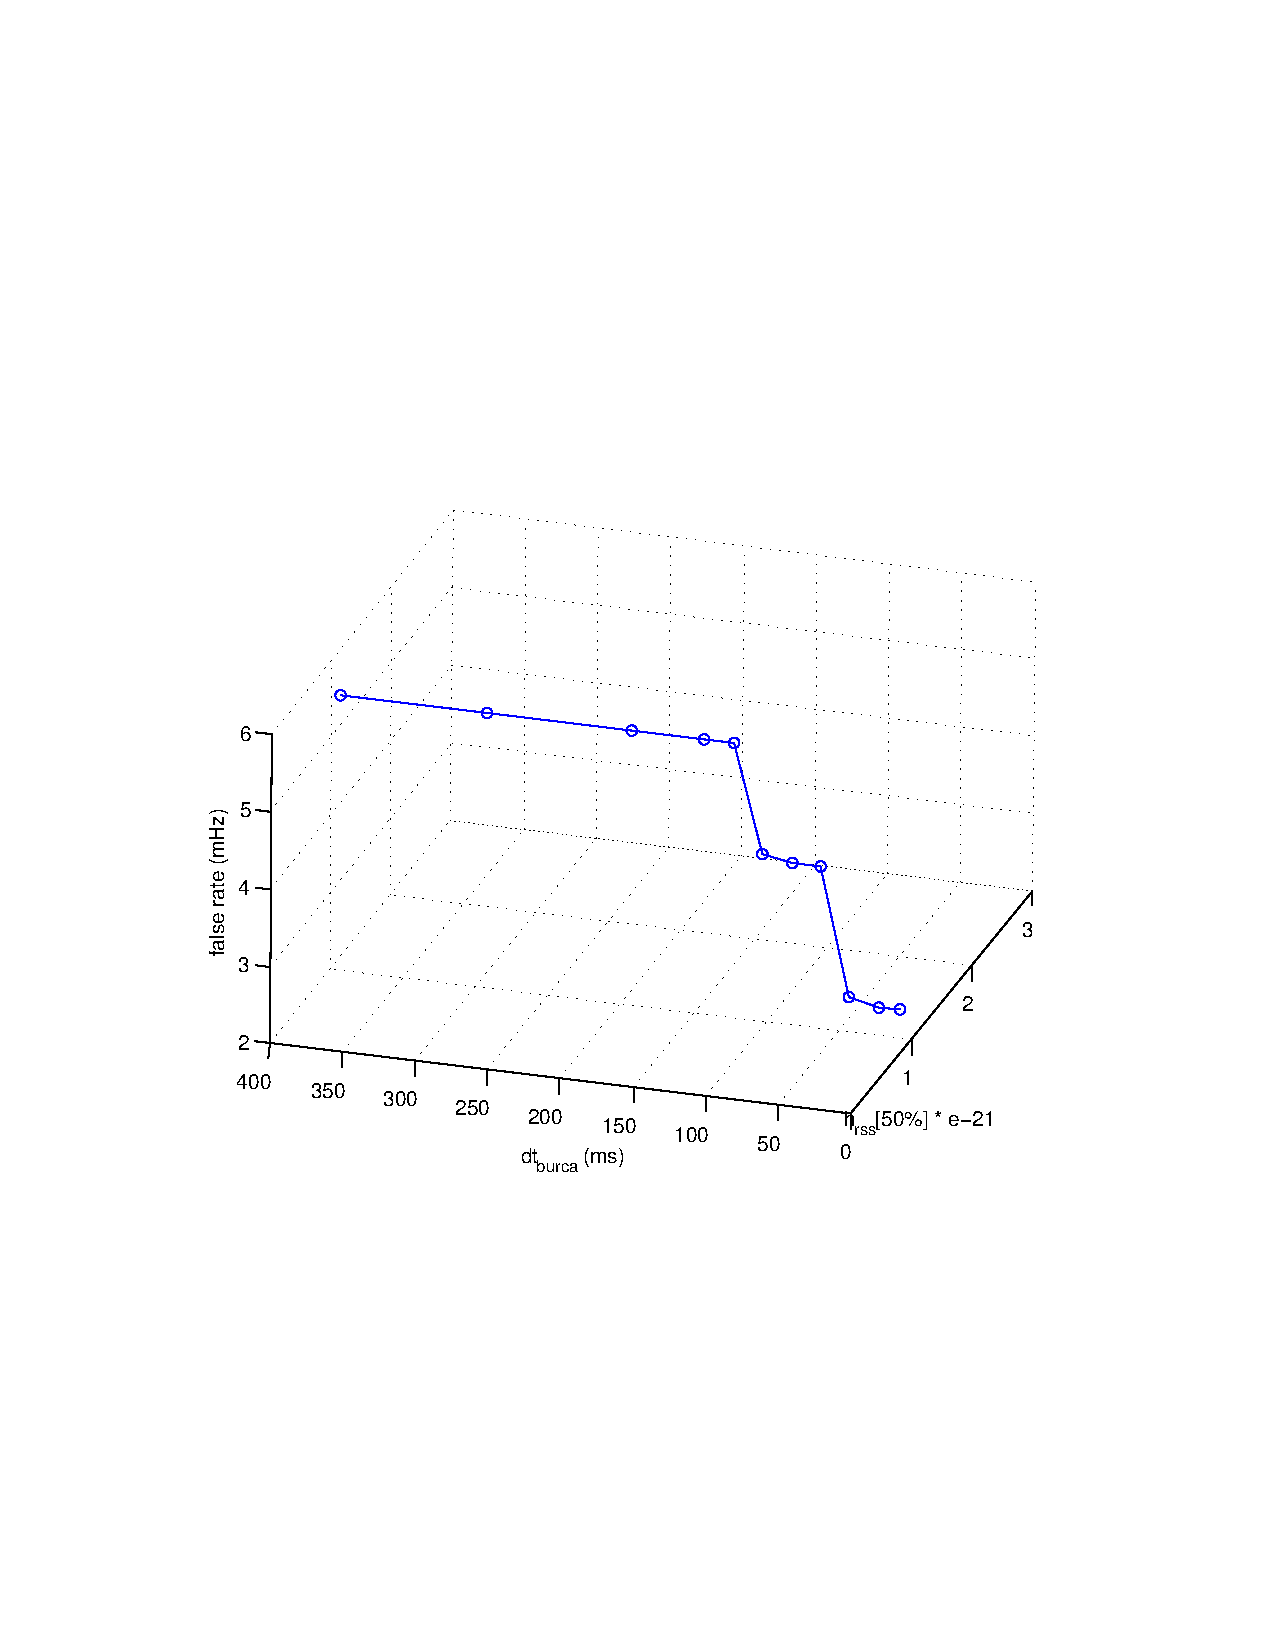
\includegraphics[width=1.0\textwidth]{figures/tune_burca_window}
\caption{Efficiency vs. False rate for different coincidence windows}
\label{fig:tuneburcawindow}
\end{center}
\end{figure} 
From the Fig~\ref{fig:tuneburcawindow} we then see that the coincidence
window has no effect in the efficicency and some minimal effects on
the false rates. This implies that our time-frequency overlap criterion
in the coincidence step has made the window length a somewhat less 
important parameter for the coincidence. Allowing a margin of error 
from sources like calibration we therefore choose the window size to be
\begin{itemize}
\item Coincidence Window: 30 ms
\end{itemize}

Here we present a set of results from S4 using the parameters tuned
as decribed in the previous sections:
\begin{itemize}
\item Fig~\ref{fig:eventsvstimelag} shows the number of false events 
at each time lag.
\item Fig~\ref{fig:sg235q9eff} shows the efficiency of the pipeline to 
$Q9$ SineGaussians at $235 Hz$. The $h_{rss}$ 50 p.c. is at $1.12e-21$.
\item Fig~\ref{fig:eobeff} shows the efficiency of the pipeline to 
EOB waveforms. The $50 p.c.$ efficiency is at $66.5 Mpc$ effective distance.   
\end{itemize}.
\begin{figure}[h]
\begin{center}
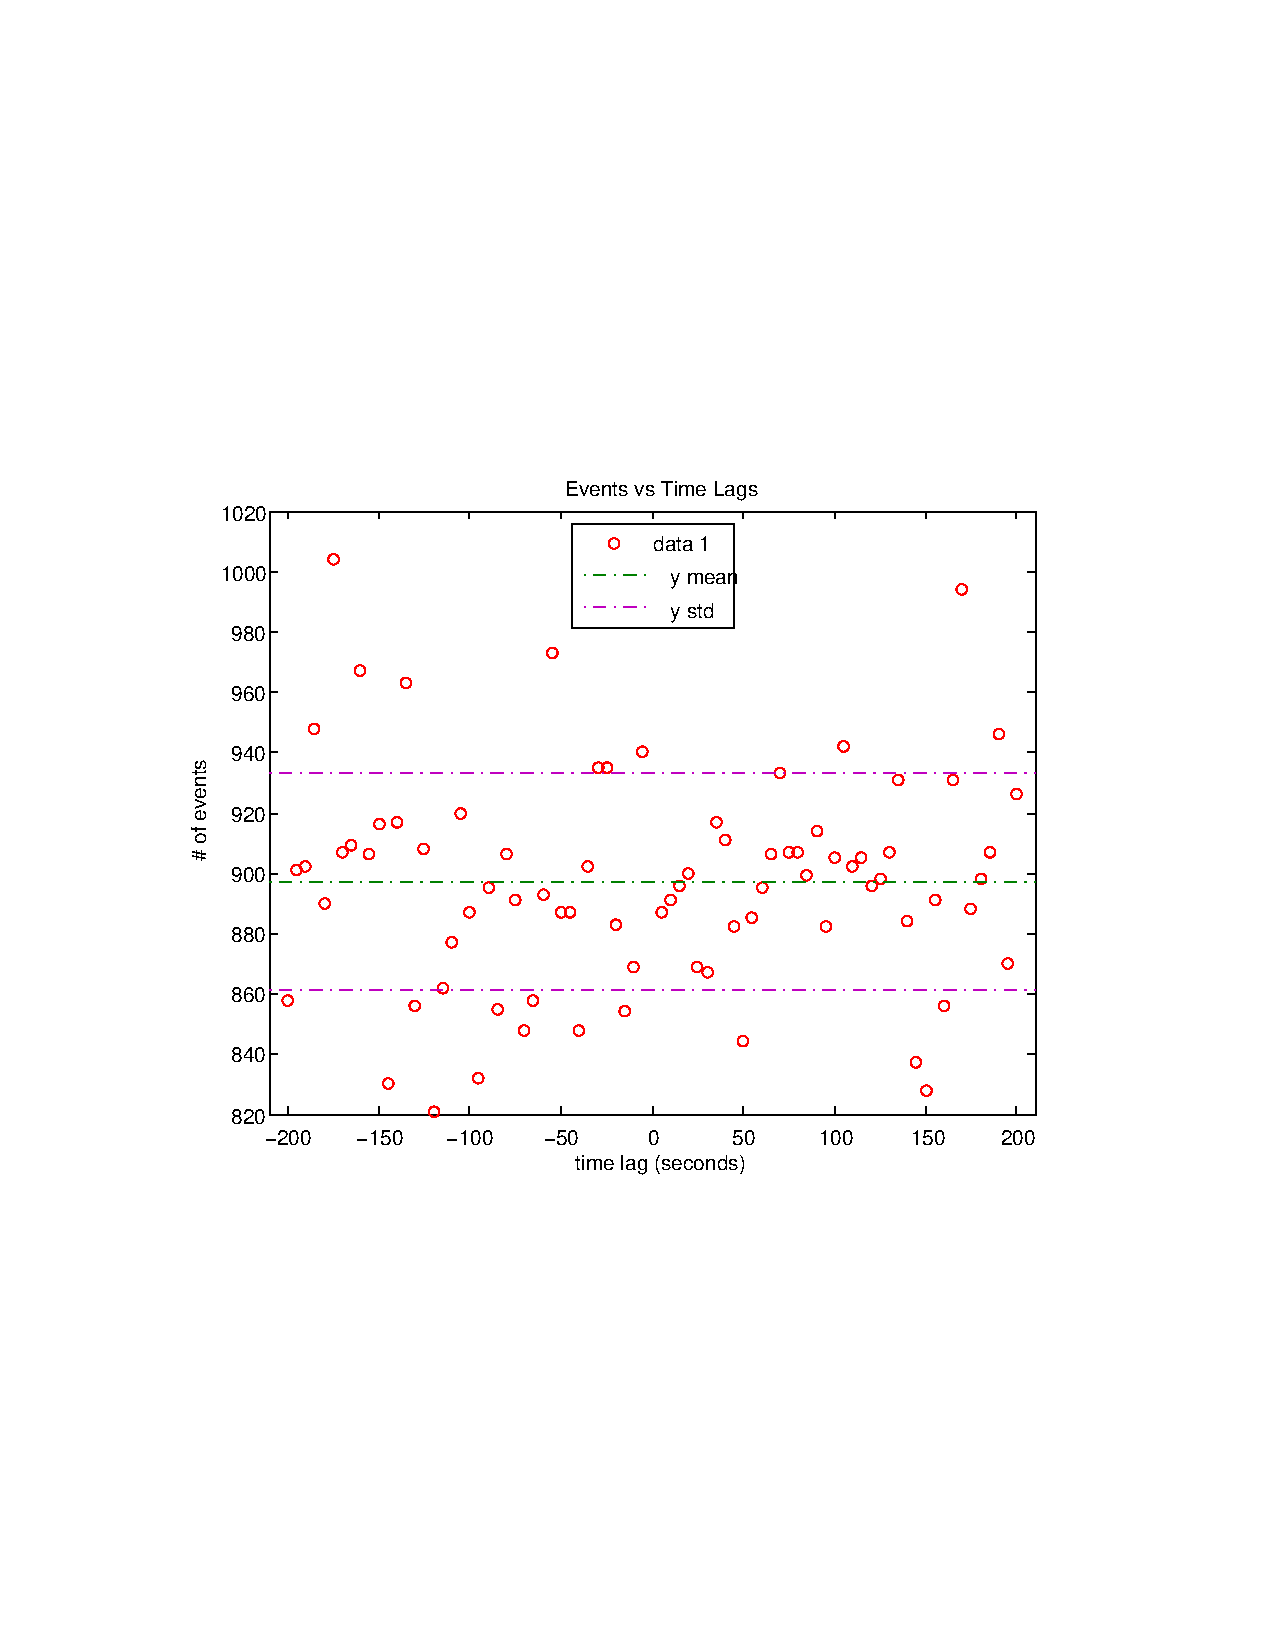
\includegraphics[width=1.0\textwidth]{figures/eventsvstimelag_20050829_1}
\caption{No. of false triggers at different time lags}
\label{fig:eventsvstimelag}
\end{center}
\end{figure}

\begin{figure}[h]
\begin{center}
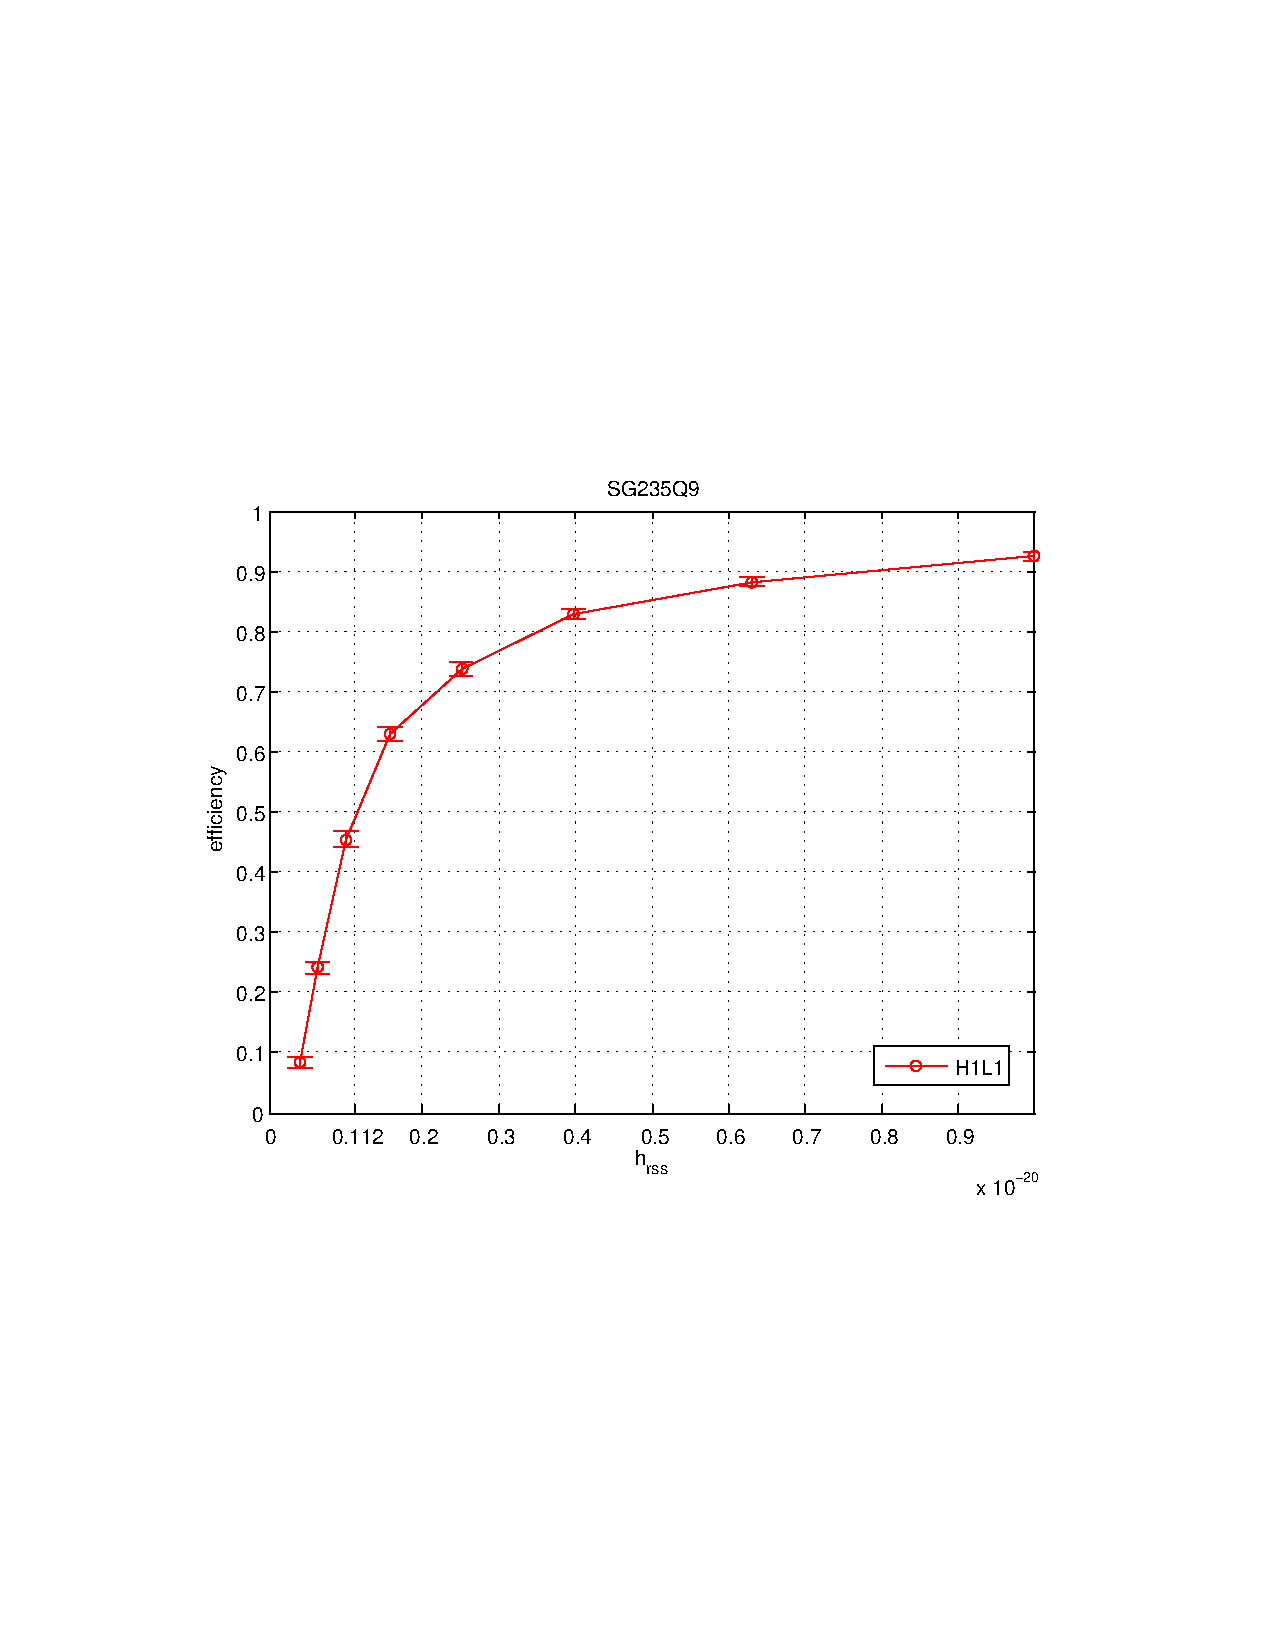
\includegraphics[width=1.0\textwidth]{figures/H1L1_eff_sg235q9_20050829_2.pdf}
\caption{Efficiency to Q9 SineGausians at 235 Hz}
\label{fig:sg235q9eff}
\end{center}
\end{figure}

\begin{figure}[h]
\begin{center}
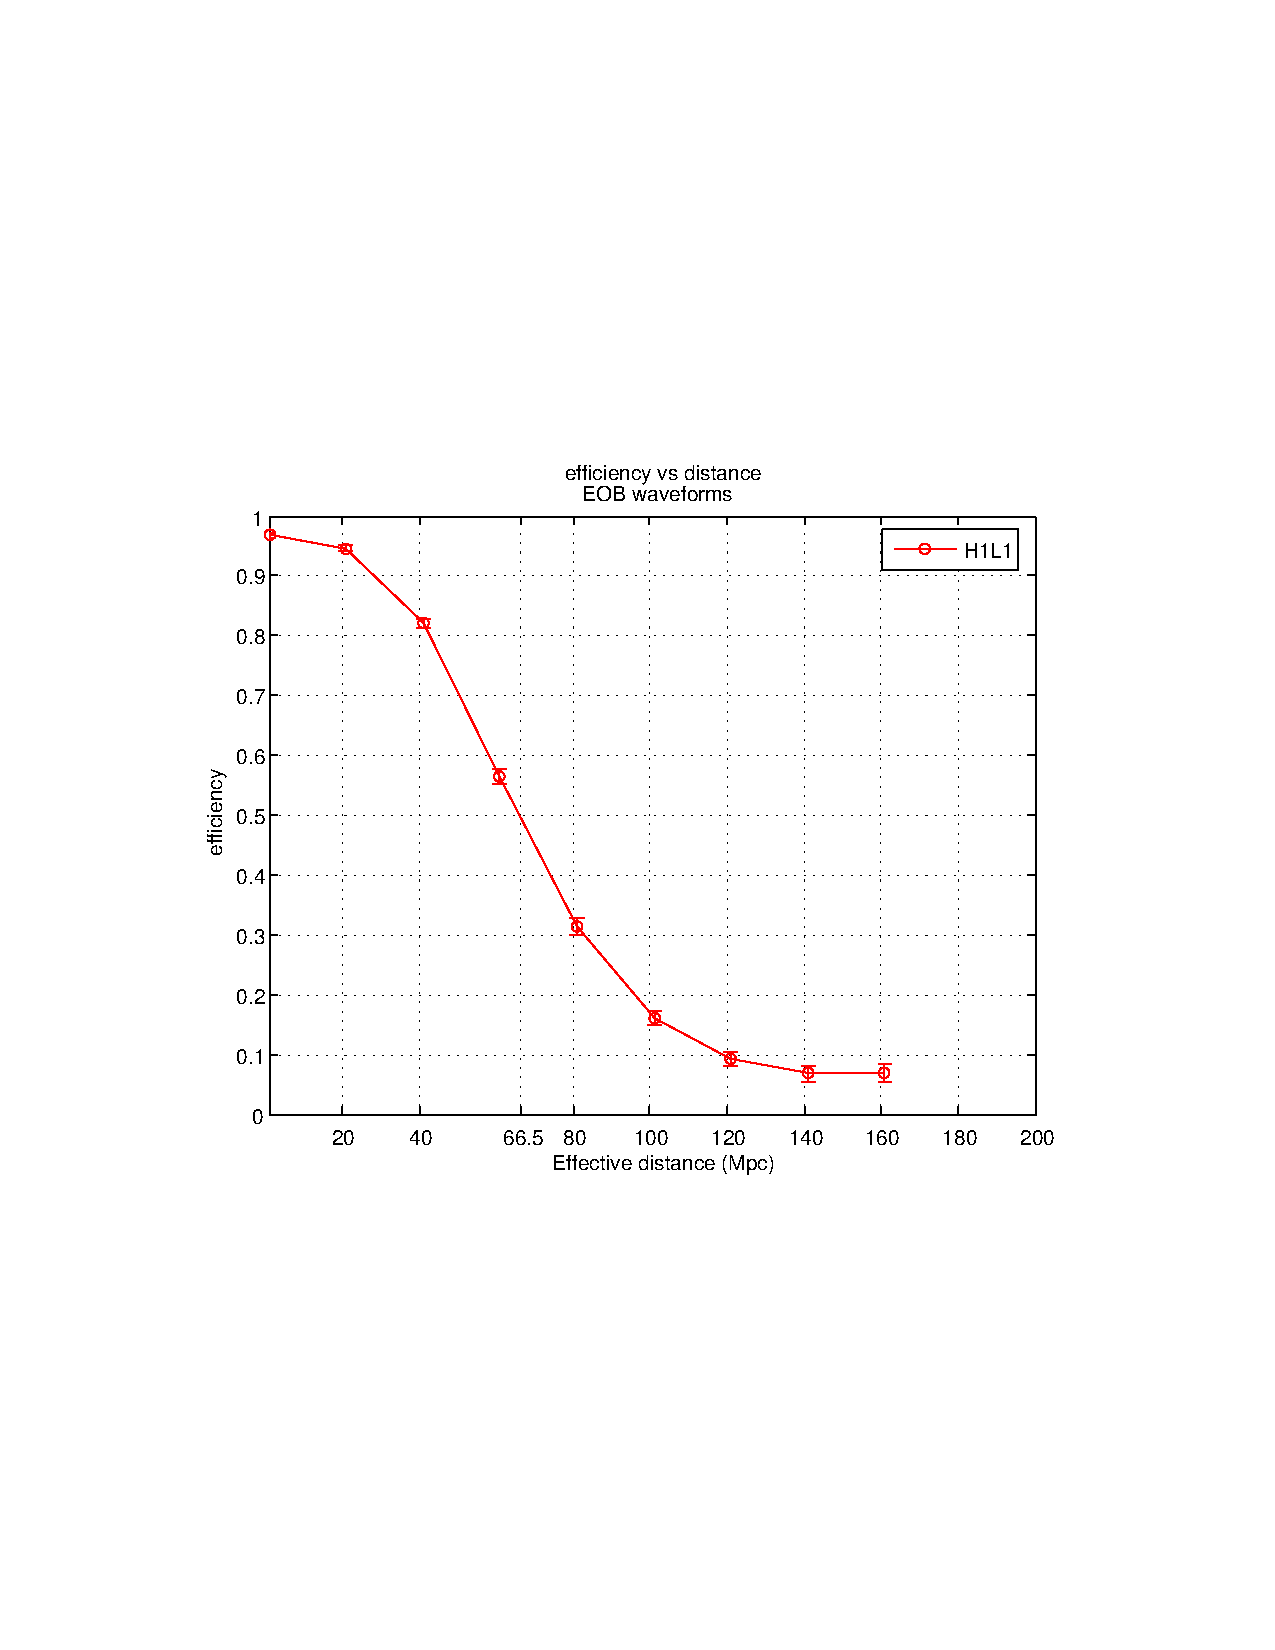
\includegraphics[width=1.0\textwidth]{figures/H1L1_eff_eob_20050829_3.pdf}
\caption{Efficiency to EOB waveforms}
\label{fig:eobeff}
\end{center}
\end{figure}

\clearpage

%%%%%%%%%%%%%%%%%%%%%%%%%%%%%%%%%%%%%%%%%%%%%%%%%%%%%%%%%%%%%%%%%%%%%
% BURCA:  coincidence analysis code
%%%%%%%%%%%%%%%%%%%%%%%%%%%%%%%%%%%%%%%%%%%%%%%%%%%%%%%%%%%%%%%%%%%%%
\section{Program \prog{lalapps\_burca}}
\label{program:lalapps-burca}
\idx[Program]{\prog{lalapps\_burca}}

\begin{entry}
\item[Name]
\prog{lalapps\_burca} --- program does burst coincidence analysis.

\item[Synopsis]
\prog{lalapps\_burca} \newline \hspace*{0.5in}
[\option{--verbose}] \newline \hspace*{0.5in}
[\option{--noplayground}] \newline \hspace*{0.5in}
[\option{--noncoincident}] \newline \hspace*{0.5in}
[\option{--ignore-playground}] \newline \hspace*{0.5in}
[\option{--ignore-tfcomparison}] \newline \hspace*{0.5in}
[\option{--ignore-tcomparison}] \newline \hspace*{0.5in}
\option{--ifo-a}~\parm{trigfile.a} \newline \hspace*{0.5in}
\option{--ifo-b}~\parm{trigfile.b} \newline \hspace*{0.5in}
[\option{--clustertype}] \newline \hspace*{0.5in}
[\option{--dt}~\parm{deltat}] \newline \hspace*{0.5in}
[\option{--start-time}~\parm{GPS seconds}] \newline \hspace*{0.5in}
[\option{--stop-time}~\parm{GPS seconds}] \newline \hspace*{0.5in}
[\option{--slide-time}~\parm{GPS seconds}] \newline \hspace*{0.5in}
[\option{--slide-time-ns}~\parm{GPS nanoseconds}] \newline \hspace*{0.5in}
[\option{--output-dir}~\parm{directory}] \newline \hspace*{0.5in}
[\option{--number-slides}~\parm{number}] \newline \hspace*{0.5in}
[\option{--user-tag}] \newline \hspace*{0.5in}
[\option{--help}] \newline \hspace*{0.5in}


\item[Description] 
\prog{lalapps\_burca} performs coincidence on triggers from the burst
search code.  It must be called with at least one input file from each 
instrument.  Currently it outputs the triggers from \option{--ifo\_a} which
are coincident with triggers from \option{--ifo\_b}.  One can also perform
time-slided background analysis by using the options \option{--slide-time},
  \option{--slide-time-ns} and \option{--number-slides}.  The output files
are of the form H1-BURCA\_H1L1\_P\_0\_H1H2-755518013-345.xml.
      

\item[Options]\leavevmode
\begin{entry}
\item[\option{--verbose}]  Displays some useful messages.

\item[\option{--noncoincident}]  Finds the non-coincident triggers and
outputs in a file of the form H1-NEGBURCA\_H1L1\_P\_0\_H1H2-755518013-345.xml.

\item[\option{--ignore-playground}] Considers all triggers independent of 
whether they are playground or non-playground. 

\item[\option{--ignore-tfcomparison}] While comparing triggers they are marked 
coincident if the triggers lie within +/- \parm{deltaT}(argument of 
\option{--dt}).

\item[\option{--ignore-tcomparison}] While comparing triggers they are marked 
coincident if the triggers lie within +/- \parm{deltaT}(argument of 
\option{--dt}) and if they overlap in frequency band.

\item[\option{--ifo-a} \parm{trigfile.a}]  LIGO lightweight XML file with
triggers from interferometer A.  This argument can be called multiple
times.  Triggers are sorted \emph{after} all files have been read in. 

\item[\option{--ifo-b} \parm{trigfile.b}]  LIGO lightweight XML file with
triggers from interferometer B.  This argument can be called multiple
times.  Triggers are sorted \emph{after} all files have been read in. 

\item[\option{--start-time} \parm{GPS seconds}]  Ignore triggers with start
times earlier than \parm{GPS seconds}.

\item[\option{--stop-time} \parm{GPS seconds}]  Ignore triggers with stop
times later than \parm{GPS seconds}.

\item[\option{--clustertype} \parm{cluster type}] Clusters the coincident 
triggers and the type of clustering is specified as an option.  The valid
types are \parm{clusterbypeaktimeandfreq, clusterbytimeandfreq}.  

\item[\option{--dt} \parm{deltat}]  Accept triggers for coincidence comparison 
if their start times agree within \parm{deltat} msec.  If not supplied,  then
\parm{deltat} = 0.

\item[\option{--slide-time} \parm{GPS seconds}] The time in GPS seconds by which 
the triggers are slided in each step for background analysis.

\item[\option{--slide-time-ns} \parm{GPS nanoseconds}] The time in GPS 
nanoseconds by which the triggers are slided in each step for background 
analysis.  The total time slided in each step is thus calculated from
both \option{--slide-time} and \option{--slide-time-ns}.

\item[\option{--number-slides} \parm{number}] Specifies the number of slides
to be performed for the background analysis.  

\item[\option{--user-tag} \parm{tag}] Optional user tag.  Gets appended to the 
output file names.

\item[\option{--noplayground}]  Record triggers in the non-playground times.  
The default behaviour returns only those triggers which lie in the playground 
data set.  

\item[\option{--help}]  Print a help message.
\end{entry}

\item[Coincidence Example]
\begin{verbatim}
lalapps_burca \
--ifo-a L-POWER-734357353-1024.xml \
--ifo-b H-POWER-734357353-1024.xml \
--dt 10 \
--start-time 734357353 \
--stop-time 734358353 \
--noplayground
\end{verbatim}

\item[Background Example]
\begin{verbatim}
lalapps_burca \
--ifo-a L-POWER-734357353-1024.xml \
--ifo-b H-POWER-734357353-1024.xml \
--dt 10 \
--slide-time 4 \
--slide-time-ns 250000000 \
--number-slides 50 \
--start-time 734357353 \
--stop-time 734358353 \
--noplayground
\end{verbatim}

\item[Author] 
Patrick Brady and Saikat Ray-Majumder
\end{entry}
\clearpage


%%%%%%%%%%%%%%%%%%%%%%%%%%%%%%%%%%%%%%%%%%%%%%%%%%%%%%%%%%%%%%%%%%%%%
% BINJ:  injection generation code
%%%%%%%%%%%%%%%%%%%%%%%%%%%%%%%%%%%%%%%%%%%%%%%%%%%%%%%%%%%%%%%%%%%%%
\section{Program \prog{lalapps\_binj}}
\label{program:lalapps-binj}
\idx[Program]{\prog{lalapps\_binj}}

\begin{entry}
\item[Name]
\prog{lalapps\_binj} --- produces burst injection data files.

\item[Synopsis]
\prog{lalapps\_binj} \newline \hspace*{0.5in}
[\option{--help}] \newline \hspace*{0.5in}
\option{--gps-start-time}~\parm{tstart} \newline \hspace*{0.5in}
\option{--gps-end-time}~\parm{tend} \newline \hspace*{0.5in}
[\option{--time-step}~\parm{tstep}] \newline \hspace*{0.5in}
[\option{--seed}~\parm{seed}] \newline \hspace*{0.5in}
[\option{--waveform}~\parm{wave}] \newline \hspace*{0.5in}
[\option{--coordinates}~\parm{coordinates}] \newline \hspace*{0.5in}
[\option{--freq}~\parm{freq}] \newline \hspace*{0.5in}
[\option{--flow}~\parm{flow}] \newline \hspace*{0.5in}
[\option{--fhigh}~\parm{fhigh}] \newline \hspace*{0.5in}
[\option{--deltaf}~\parm{deltaf}] \newline \hspace*{0.5in}
[\option{--quality}~\parm{quality}] \newline \hspace*{0.5in}
[\option{--tau}~\parm{tau}] \newline \hspace*{0.5in}
[\option{--hpeak}~\parm{hpeak}] \newline \hspace*{0.5in}
[\option{--log-hpeak-min}~\parm{log-hpeak-min}] \newline \hspace*{0.5in}
[\option{--log-hpeak-max}~\parm{log-hpeak-max}] \newline \hspace*{0.5in}
[\option{--max-distance}~\parm{max-distance}] \newline \hspace*{0.5in}
[\option{--min-distance}~\parm{min-distance}] \newline \hspace*{0.5in}
[\option{--simwaveform-duration}~\parm{simwaveform-duration}] \newline \hspace*{0.5in}
[\option{--simwaveform-min-number}~\parm{simwaveform-min-number}] \newline \hspace*{0.5in}
[\option{--simwaveform-max-number}~\parm{simwaveform-max-number}] \newline \hspace*{0.5in}
[\option{--usertag}~\parm{tag}]

\item[Description] 
\prog{lalapps\_binj} generates a number of burst  parameters suitable  for
using in a Monte Carlo injection to test the efficiency of a burst search.
The  various parameters (detailed  below)  are specified on the command
line or can be randomly chosen in a manner appropriate for an burst upper
limit search.

The longitude $\alpha$ of the source is uniformly distributed in the range
$[0,2\pi]$, the latitude $\delta$ is defined so that $\cos(\pi/2 - \delta)$
is uniformly distributed in the range $[-1,1]$,  and the polarization angle
$\psi$  is uniformly distributed in the range $[0,2\pi]$.

The output of this program  is  a  list  of  the  injected events,
starting at  the specified start time, ending at the specified end time,
and containing one set  of burst parameters every specified time step.  The
output is written to a file name in the standard burst pipeline format:
\begin{center}
\begin{verbatim}
        HL-INJECTIONS_USERTAG_SEED-GPSSTART-DURATION.xml
\end{verbatim}
\end{center}
where \verb$USERTAG$ is \parm{tag} as specfied on the command line,
\verb$SEED$ is the  value  of  the random number seed chosen and
\verb$GPSSTART$ and \verb$DURATION$ describes the GPS time interval that
the file covers. The file is in the standard LIGO lightweight XML format
containing a \texttt{sim\_burst} table that describes the injections.  This
table is described in the LAL \texttt{tools} package under
\texttt{LIGOMetadataTables.h} header.  

The output is also written to an ascii file named in the following way:
\begin{center}
\begin{verbatim}
        HLT-INJECTIONS_USERTAG_SEED-GPSSTART-DURATION.txt
\end{verbatim}
\end{center}
where \verb$USERTAG$ is \parm{tag} as specfied on the command line,
\verb$SEED$ is the  value  of  the random number seed chosen and
\verb$GPSSTART$ and \verb$DURATION$ describes the GPS time interval that
the file covers. The file is in the format agreed to for LIGO-TAMA
simulations.  

If a \option{--user-tag} is not specified on the command line, the
\texttt{\_USERTAG} part of the filename will be omitted.

\item[Options]\leavevmode
\begin{entry}
\item[\option{--help}] Print a help message.

\item[\option{--gps-start-time} \parm{tstart}]
Optional.  Start time of the injection data to be created. Defaults to the
start of S2, Feb 14 2003 16:00:00 UTC (GPS time 729273613)

\item[\option{--gps-end-time} \parm{tend}]
Optional. End time of the injection data to be created. Defaults to the end
of S2, Apr 14 2003 15:00:00 UTC (GPS time 734367613).

\item[\option{--time-step} \parm{tstep}]
Optional. Sets the time step interval between injections. The injections
will occour at \parm{tstep}$/\pi$ second intervals. Defaults to $2630/\pi$.

\item[\option{--seed} \parm{seed}]
Optional. Seed the random number generator with the integer \parm{seed}.
Defaults to $1$.

\item[\option{--coordinates} \parm{coordinates}] 
Optional.  The coordinate system to specify for the injections.  Use one
of:
\begin{itemize}
\item \texttt{GEOGRAPHIC}
\item \texttt{EQUATORIAL}
\item \texttt{ECLIPTIC}
\item \texttt{GALACTIC}
\item \texttt{ZENITH}
\end{itemize}
The default is \texttt{EQUATORIAL}.   Use \texttt{ZENITH} to describe an
injection from directly above the detector with linear polarization with
respect to the detector.  Note:  this is different than using
\texttt{HORIZON} coordinates since the polarization angle is usually
defined with respect to geo-centric coordinates.

\item[\option{--flow} \parm{flow}]
Optional.  The code can generate injections at multiple frequencies.  This
option sets the first frequency used in that case.  Default value is 150
Hz.

\item[\option{--fhigh} \parm{fhigh}]
Optional.  Only generate injections with frequencies below \parm{fhigh}.
Default value is 1000 Hz.

\item[\option{--deltaf} \parm{deltaf}]
Optional.  The linear spacing between frequencies used to make
injections.  Default value is 0 Hz.

\item[\option{--waveform} \parm{wave}]
Optional.  Default is \texttt{SineGaussian}.   The string \parm{wave} will
be written into the \texttt{waveform} column of the \texttt{sim\_burst}
table output. This is used by the burst code to determine which type of
waveforms it should inject into the data.  Types implemented in LAL inject
package are:
\begin{description}
\item[\texttt{SineGaussian}]  Inject a sine-Gaussian waveform defined by
\begin{eqnarray}
A_+(t) &=& h_0 \exp[ - (t-t_0)^2/ \tau^2 ] \sin[ 2 \pi f_0 (t-t_0)] \\
A_\times(t) &=& 0
\end{eqnarray}

\item[\texttt{CosGaussian}]  Inject a cos-Gaussian waveform defined by
\begin{eqnarray}
A_+(t) &=& h_0 \exp[ - (t-t_0)^2/ \tau^2 ] \cos[ 2 \pi f_0 (t-t_0)] \\
A_\times(t) &=& 0
\end{eqnarray}
\end{description}

\item[\option{--tau} \parm{tau}]
Optional.  The decay-time $\tau$ for sine-gaussian,  gaussian,  ringdown
and ring-up waveforms.

\item[\option{--quality} \parm{quality}]
Optional.  The quality factor for sine-gaussian,  gaussian,  ringdown and
ring-up waveforms.    This option overrides the decay-time \parm{tau} and
recalculates the duration for each waveform using the formula
$$ 
\tau = \frac{\textsc{quality} }{ \sqrt{2} \pi f_0 }
$$
where $f_0$ is the frequency of the injection.

\item[\option{--freq} \parm{freq}]
Optional.  The central frequency $f_0$ for sine-gaussian,  ringdown and
ring-up waveforms.

\item[\option{--hpeak} \parm{hpeak}]
Optional.  The peak dimensionless strain $h_0$ for sine-gaussian,
gaussian,  ringdown and ring-up waveforms.

\item[\option{--log-hpeak-min} \parm{log-hpeak-min}]
Optional.  When this option is invoked,  a range of values of $h_0$ such
that $\log_{10}(h_0)$ is uniformly distributed in the range
$[$\parm{log-hpeak-min}$, $\parm{log-hpeak-max}$]$.  If this option is
used, then \option{--log-hpeak-max} is required.

\item[\option{--log-hpeak-max} \parm{log-hpeak-max}]
Optional.  When this option is invoked,  a range of values of $h_0$ such
that $\log_{10}(h_0)$ is uniformly distributed in the range
$[$\parm{log-hpeak-min}$, $\parm{log-hpeak-max}$]$.  If this option is
used, then \option{--log-hpeak-min} is required.

\item[\option{--user-tag} \parm{string}]
Optional. Set the user tag for this job to be \parm{string}. May also be
specified on the command line as \option{-userTag} for LIGO database
compatibility.

\item[\option{--max-distance} \parm{distance}]
Optional.  This is used when one wants to inject simulated Inspiral$+$Burst$+$Ringdown 
waveforms.  This specifies the maximum distance in Kpc that a source can be placed at.
This should be used with the \option{--min-distance}.

\item[\option{--min-distance} \parm{distance}]
Optional.  This is used when one wants to inject simulated Inspiral$+$Burst$+$Ringdown 
waveforms.  This specifies the minimum distance in Kpc that a source can be placed at.
This should be used with the \option{--max-distance}.

\item[\option{--d-distr} \parm{distribution number}] 
Optional.  This is used when the maximum and minimum distribution options are used.
 This should be an integer number and depending on the number different distance
distributions can be used while placing the sources.  

\item[\option{--simwaveform-duration} \parm{simwaveform-duration}]
Optional.  This specifies the duration in seconds of the frames containing the simulated 
waveforms.

\item[\option{--simwaveform-min-number} \parm{simwaveform-min-number}] 
Optional.  This specifies the minimum number of the simulated waveforms to be injected.

\item[\option{--simwaveform-max-number} \parm{simwaveform-max-number}] 
Optional.  This specifies the maximum number of the simulated waveforms to be injected.  
\end{entry}

\item[Example]
\begin{verbatim}
lalapps_binj \
--time-step 1000 \
--flow 130 \
--fhigh 600 \
--deltaf 90 \
--quality 8.89 \
--hpeak 6.0e-20 \
--seed 45
\end{verbatim}

\item[Author] 
Jolien Creighton, Patrick Brady, Duncan Brown, Saikat Ray-Majumder
\end{entry}
\clearpage


%%%%%%%%%%%%%%%%%%%%%%%%%%%%%%%%%%%%%%%%%%%%%%%%%%%%%%%%%%%%%%%%%%%%%
% BINJ_FIND:  injection finding code
%%%%%%%%%%%%%%%%%%%%%%%%%%%%%%%%%%%%%%%%%%%%%%%%%%%%%%%%%%%%%%%%%%%%%
\section{Program \prog{lalapps\_binj\_find}}
\label{program:lalapps-binj-find}
\idx[Program]{\prog{lalapps\_binj\_find}}

\begin{entry}
\item[Name]
\prog{lalapps\_binj\_find} --- Finds the triggers corresponding to injections.

\item[Synopsis]
\prog{lalapps\_binj\_find} \newline \hspace*{0.5in}
[\option{--verbose}] \newline \hspace*{0.5in}
[\option{--printresult}] \newline \hspace*{0.5in}
[\option{--playground}] \newline \hspace*{0.5in}
[\option{--noplayground}] \newline \hspace*{0.5in}
[\option{--best-confidence}] \newline \hspace*{0.5in}
[\option{--best-peaktime}] \newline \hspace*{0.5in}
[\option{--help}] \newline \hspace*{0.5in}
\option{--input-trig}~\parm{trigger file} \newline \hspace*{0.5in}
\option{--input-burstinj}~\parm{burst injection file} \newline \hspace*{0.5in}
[\option{--input-inspinj}~\parm{inspiral injection file}] \newline \hspace*{0.5in}
\option{--output-inj-made}~\parm{output injection} \newline \hspace*{0.5in}
[\option{--max-confidence}~\parm{max confidence}] \newline \hspace*{0.5in}
\option{--gps-start-time}~\parm{tstart} \newline \hspace*{0.5in}
\option{--gps-end-time}~\parm{tend} \newline \hspace*{0.5in}
[\option{--min-centralfreq}~\parm{min centralfreq}] \newline \hspace*{0.5in}
[\option{--max-centralfreq}~\parm{max centralfreq}] \newline \hspace*{0.5in}
\option{--output-inj-found}~\parm{output inj made} \newline \hspace*{0.5in}
\option{--compare-choice}~\parm{compare choice} \newline \hspace*{0.5in}
\option{--output-trig}~\parm{output-trig} \newline \hspace*{0.5in}

\item[Description] 
\prog{lalapps\_binj\_find} finds the triggers which correspond to an injection.


It takes in the list of injections that were generated by the \prog{lalapps\_binj} 
and first checks if the time of an injection is within times
for which triggers have been generated.  If triggers were generated then the program 
scans through the list of triggers produced by the pipeline searching for one
which corresponds to the injection.  Then this comparison is repeated for all the 
injections in the list.

The method of comparison is decided by the \option{--compare-choice}.  By default
the program checks if the time and frequency of the injection lies inside the 
time-frequency tile of the trigger.  One can also choose to compare if only the
time of the injection lies inside the time duration of the trigger.  However in the
case of waveforms which do not have a characteristic frequency only the time comparison 
is done.
 
The outputs of the program are in three seperate files: one containing the list of the 
injections that were actually made,  one containing the list of injections that were found
and the other containing the list of triggers which correspond to the injections that were 
found.  Let us explain the contents of the first file a bit more.  \prog{lalapps\_binj}
produces a list of injections all of which may not be actually analysed,  for eg.
analysis of a particular stretch of data may fail for some reason while injections were 
listed for those times.  So to count the number of injections that were actually made
one should account for the failed jobs.  The argument to \option{--output-inj-made} in
fact contains this list of injections that were actually made.
   

\item[\option{--verbose}]
Optional.  Print useful information while executing the code.

\item[\option{--printresult}]
Optional.  Writes the number of injections that were made and the number that were found with
the total time that was analyzed.

\item[\option{--playground}]
Optional.  Compare injections and triggers iff they lie in the playground times.

\item[\option{--noplayground}]
OPtional.  Compare injections and triggers iff they lie outside the playground times. 

\item[\option{--best-confidence}]
Optional.  When multiple triggers are found corresponding to a single injection,  the
one with the maximum confidence is marked as the trigger corresponding to the injection.

\item[\option{--best-peaktime}]
Optional.  When multiple triggers are found corresponding to a single injection,  the
one with the peak time matching most closely with the injection time is marked as the 
trigger corresponding to that particular injection.

\item[\option{--help}]
Optional.  Prints the usage information.

\item[\option{--input-trig} \parm{trigfile}]
This is a .txt file containing the list of .xml trigger files produced by the pipeline.
The trigger files listed in the txt file are then searched for triggers matching the 
injections.

\item[\option{--input-burstinj} \parm{injection file}]
This is a .txt file containing the list of .xml injection files produced by the 
\prog{lalapps\_binj}. The injections in the files listed in the txt file are then 
compared with the triggers produced by the pipeline to find matching triggers.

\item[\option{--input-inspinj} \parm{injection file}]
This is a .txt file containing the list of .xml injection files produced by the 
\prog{lalapps\_bbhinj}. The injections in the files listed in the txt file are then searched 
for compared with the triggers produced by the pipeline to find matching triggers.

\item[\option{--output-inj-made} \parm{made injection file}]
This file contains the list of injections that were actually made.

\item[\option{--max-confidence} \parm{max-confidence}]
The triggers having a confidence lower than max-confidence are only concidered for
the comparison with the injections.

\item[\option{--gps-start-time} \parm{gps-start-time}]
The triggers and injections are considered for comparison if only they occur at times after 
the gps time specified as this option.

\item[\option{--gps-start-time} \parm{gps-end-time}]
The triggers and injections are considered for comparison if only they occur at times before 
the gps time specified as this option.

\item[\option{--min-centralfreq} \parm{min-centralfreq}]
Optional.  Triggers are only considered for comparison if they have central frequency more than the 
frequency specified as this option.

\item[\option{--max-centralfreq} \parm{max-centralfreq}]
Optional.  Triggers are only considered for comparison if they have central frequency less than the 
frequency specified as this option.

\item[\option{--output-inj-found} \parm{output-inj-found}]
This file contains the list of injections that were found to have a corresponding trigger.

\item[\option{--compare-choice} \parm{compare-choice}]
This specifies the different types of comparisons that may be performed while searching 
for triggers corresponding to an injection. As of now the compare-choices are 
\parm{comparebytimeandfreq, comparebytime}.  By default the choice is \parm{comparebytimeandfreq}, 
when both time and frequency are compared to determine if an injection has been found.  The other
choice is \parm{comparebytime} when only the time is compared for the detection purpose.

\item[\option{--output-trig} \parm{output-trig}]
This file contains the list of triggers that are found matching with some injections.

\item[Example]
\begin{verbatim}
lalapps_binj_find \
--input-trig H1.txt \
--input-burstinj burstinj.txt \
--output-trig H1.xml \
--output-inj-made H1injmade.xml \
--output-inj-found H1injfound.xml \
--best-peaktime \
--gps-start-time 753601043 \
--gps-end-time 757346760 \
--printresult \
--compare-choice comparebytimeandfreq
\end{verbatim}

\item[Author] 
Patrick Brady, Saikat Ray-Majumder
\end{entry}
\clearpage


%%%%%%%%%%%%%%%%%%%%%%%%%%%%%%%%%%%%%%%%%%%%%%%%%%%%%%%%%%%%%%%%%%%%%
% bread:  trigger file manipulation
%%%%%%%%%%%%%%%%%%%%%%%%%%%%%%%%%%%%%%%%%%%%%%%%%%%%%%%%%%%%%%%%%%%%%
\section{Program \prog{lalapps\_bread}}
\label{program:lalapps-bread}
\idx[Program]{\prog{lalapps\_bread}}

\begin{entry}
\item[Name]
\prog{lalapps\_bread} -- reads in triggers from multiple xml files into one
single xml file 

\item[Synopsis]
\prog{lalapps\_bread} \newline \hspace*{0.5in}
[\option{--help}] \newline \hspace*{0.5in}
\option{--input}~\parm{filename} \newline \hspace*{0.5in}
\option{--output}~\parm{filename} \newline \hspace*{0.5in}
[\option{--outtxt}~\parm{filename}] \newline \hspace*{0.5in}
[\option{--max-confidence}~\parm{maximum conf}] \newline \hspace*{0.5in}
[\option{--noplayground}] \newline \hspace*{0.5in}
[\option{--sort}] \newline \hspace*{0.5in}
[\option{--cluster}] \newline \hspace*{0.5in}
[\option{--min-duration}~\parm{min dur}] \newline \hspace*{0.5in}
[\option{--max-duration}~\parm{max dur}] \newline \hspace*{0.5in}
[\option{--min-centralfreq}~\parm{min centralfreq}] \newline \hspace*{0.5in}
[\option{--max-centralfreq}~\parm{max centralfreq}] \newline \hspace*{0.5in}
[\option{--max-bandwidth}~\parm{max bw}] \newline \hspace*{0.5in}
[\option{--min-bandwidth}~\parm{min bw}] \newline \hspace*{0.5in}
[\option{--min-amplitude}~\parm{min amp}] \newline \hspace*{0.5in}
[\option{--max-amplitude}~\parm{max amp}] \newline \hspace*{0.5in}
[\option{--min-snr}~\parm{min snr}] \newline \hspace*{0.5in}
[\option{--max-snr}~\parm{max snr}] \newline \hspace*{0.5in}
[\option{--min-start-time}~\parm{min start time}] \newline \hspace*{0.5in}
[\option{--max-start-time}~\parm{max start time}] \newline \hspace*{0.5in}
[\option{--globtrig}] \newline \hspace*{0.5in}
[\option{--verbose}]

\item[Description] 
\prog{lalapps\_bread} reads in triggers from multiple xml files, does any
requested cuts specified by the user and then writes the triggers in a
single xml file.  

\item[Options]\leavevmode
\begin{entry}
\item[\option{--help}] Print a help message.

\item[\option{--input} \parm{cache file}]
Obtain the locations of input \texttt{.xml} trigger files from the LAL
cache file \parm{cache file}.  LAL cache files are explained in the
``framedata'' package in LAL and can be constructed by making calls to
\prog{LSCDataFind} on some systems.  


\item[\option{--output} \parm{filename}]
\prog{lalapps\_bread} writes all the triggers out in one single xml file,
specified by filename.  The (old) option \option{--outfile} can also be
used.

\item[\option{--outtxt} \parm{filename}]
Optional.  If this option is specified \prog{lalapps\_bread} writes all the 
triggers out in one single txt file, specified by filename. 

\item[\option{--max-confidence} \parm{maximum conf}]
Optional. Outputs only the triggers with a confidence less than or equal to
the given value.

\item[\option{--noplayground}]
Optional. By default only triggers lying inside the playground are output.
If this option is specified then all the triggers will be output. 

\item[\option{--sort}]
Not properly implemented yet. Now the triggers are always sorted in time
before being written out.

\item[\option{--cluster}]
Apply the LAL SnglBurstTable clustering algorithm to the triggers before
applying any cuts.  This is the same algorithm used by
\prog{lalapps\_power}.  Running \prog{lalapps\_power} without clustering,
followed by a clustering pass with \prog{lalapps\_bread} is equivalent to
applying clustering in \prog{lalapps\_power}.

\item[\option{--min-duration} \parm{duration}]
Optional. Outputs only the triggers with a duration greater than or equal
to the value specified.

\item[\option{--max-duration} \parm{duration}]
Optional. Outputs only the triggers with a durations less than or equal to
the value specified.

\item[\option{--min-centralfreq} \parm{frequency}]
Optional. Outputs only the triggers with a central frequency greater than
or equal to the value specified.

\item[\option{--max-centralfreq} \parm{frequency}]
Optional. Outputs only the triggers with a central frequency less than or
equal to the value specified.

\item[\option{--min-bandwidth} \parm{bandwidth}]
Optional. Outputs only the triggers with a bandwidth greater than or equal
to the value specified.

\item[\option{--max-bandwidth} \parm{bandwidth}]
Optional. Outputs only the triggers with a bandwidth less than or equal to
the value specified.

\item[\option{--min-amplitude} \parm{amplitude}]
Optional. Outputs only the triggers with an amplitude greater than or equal
to the value specified.

\item[\option{--max-amplitude} \parm{amplitude}]
Optional. Outputs only the triggers with an amplitude less than or equal to
the value specified.

\item[\option{--min-snr} \parm{snr}]
Optional. Outputs only the triggers with a SNR greater than or equal to the
value specified.

\item[\option{--max-snr} \parm{snr}]
Optional. Outputs only the triggers with a SNR less than or equal to the
value specified.

\item[\option{--min-start-time} \parm{time}]
Optional. Outputs only the triggers with a start time later than or equal
to the time specified.

\item[\option{--max-start-time} \parm{time}]
Optional. Outputs only the triggers with a start time earlier than or equal
to the time specified.

\item[\option{--globtrig} \parm{globtrig}]
Optional.  When this option is specified with the directory containing the 
triggers in it as an argument the \prog{lalapps\_bread} globs the triggers
from the directory and writes to an output file as specified.
   
\item[\option{--verbose}]
Optional. Prints out detailed message as the program runs including the
total no. of triggers.

\end{entry}

\item[Example]
\begin{verbatim}
lalapps_bread \
--input H1.txt \
--output H1.xml \
--max-confidence -50 \
--verbose
\end{verbatim}

\item[Author] 
Patrick Brady, Saikat Ray Majumder, Kipp Cannon
\end{entry}
